
% \pagebreak
% \chapter*{Educational Outreach}
% \markboth{Educational Outreach}{Educational Outreach}

% \addcontentsline{toc}{chapter}{Educational Outreach}
% \section*{About the Department:}
% \addtocounter{section}{1}
% \addcontentsline{toc}{section}{About the Department}
% Educational Outreach is the department of NSS, IITB that strives to ensure that every child receives the formal education she or he is entitled to. We at Educational Outreach believe that lack of education is one of the biggest root cause of all existing problems in the society. Also, acknowledging the fact that formal education is not enough for the all-round development of a child, initiatives like Muskaan and Prayog were started to train the students in extra-curricular activities and to develop their scientific temperament respectively. Also, this department has national outreach due to its YouTube channel, Open Learning Initiative. Voice for Purpose is another online initiative wherein books, travel diaries and current affairs news are recorded as audio books for the blind students. With a new initiative - Neem Schools for this year, which focuses on value education as the most important aspect of education, this department is constantly trying to make overall learning more fun, interesting and enriching. From the mess workers of the institute to the children of
% remote parts of India, the beneficiaries of this department are varied and large in number.



% \section*{Initiatives:}
% \addtocounter{section}{1}
% \addcontentsline{toc}{section}{Initiatives}

% \noindent \textbf{\Large Open Learning Initiative:}
% \addcontentsline{toc}{subsection}{Open Learning Initiative} \\ \\ \noindent \textbf{About the initiative:} OLI is a You Tube channel that was launched by NSS, IITB to ensure that language does not become a barrier in
% education. With educational videos recorded by our volunteers (mostly UG students in their first, second or third years)
% in regional languages, we aim to make the Internet equally useful for students who don’t study in English medium
% schools. Currently, the channel contains 250+ educational videos on Science and Mathematics in eight Indian languages,
% namely, Hindi, Marathi, Gujarati, Bengali, Odia, Malayalam, Tamil, and Telugu. There is also a course on English to
% benefit the students and a section on scientific experiments, wherein interesting and informative experiments are
% demonstrated to enhance the interest of the students in science and to promote scientific temperament and another
% section on fun facts and interesting concepts(Edutainment).\\

% \noindent \textbf{Link: } \url{http://youtube.com/c/OLINSSIITB} \\


% \noindent \textbf{Ideation:} The idea of launching this YouTube channel was born out of a discussion with a nearby NGO, Vidya. They were on the lookout for educational videos in Hindi and Marathi. They had AV facilities and hence they could have shown those videos to students in the absence of teachers. However, thorough search on the internet did not produce satisfactory results and most of the good videos were in English. That's when we thought of starting our own YouTube channel.\\

% \begin{figure}[H]
% \centering
% 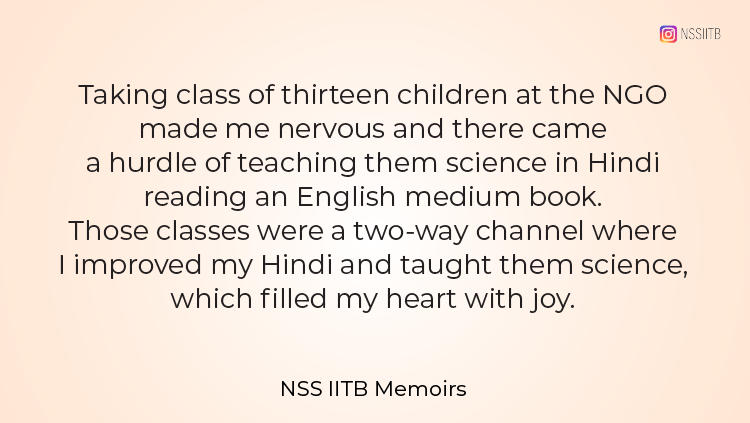
\includegraphics[width = 0.5\textwidth]{3.png}
% \caption*{Homepage of the OLI channel on YouTube}
% \end{figure}

% \noindent \textbf{Outreach:} The growth of OLI has been exponential in the last year. Starting from 300 subscribers, OLI has grown to
% about 50k subscribers and 4.2 million+ views. Many NGOs in Powai like Vidya, Asha, Logic Center and Community
% Welfare Association (LCCWA) etc. are using our videos for teaching their students. LCCWA has regular OLI sessions for
% students on Tuesdays and Thursdays. Many people from other parts of the nation have also been availing our resources.This is what Diwakaran sir from LCCWA had to say about OLI:\\ \\
% \textit{``OLI is a fantastic tool for learning Math specially for 8th std students. As it is in Hindi language and is for the vernacular medium, it is very easy for them to understand the concepts"}\\


% \begin{figure}[H]
% \centering
% 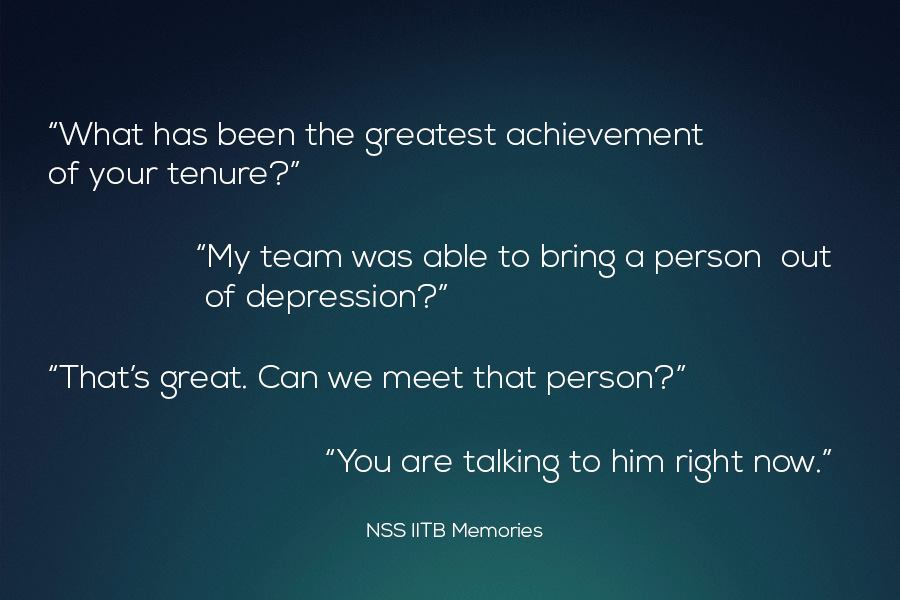
\includegraphics[width = 0.8\textwidth]{4.jpg}
% \caption*{Disha – an E-learning program in Giridih, Jharkhand using OLI videos}
% \end{figure}

% \noindent \textbf{Long-term goals:}
% \begin{itemize}
% \item Cover all the major regional languages of India
% \item Reach out to as many NGOs as possible.
% \item Cover all the basic topics in Science and Math and also other subjects
% \item Train the students in English and make them proficient in the language so that they don't face any problems in their higher studies and professional life
% \item Make learning fun and interesting\\ \\
% \end{itemize}

% \begin{figure}[H]
% \centering
% 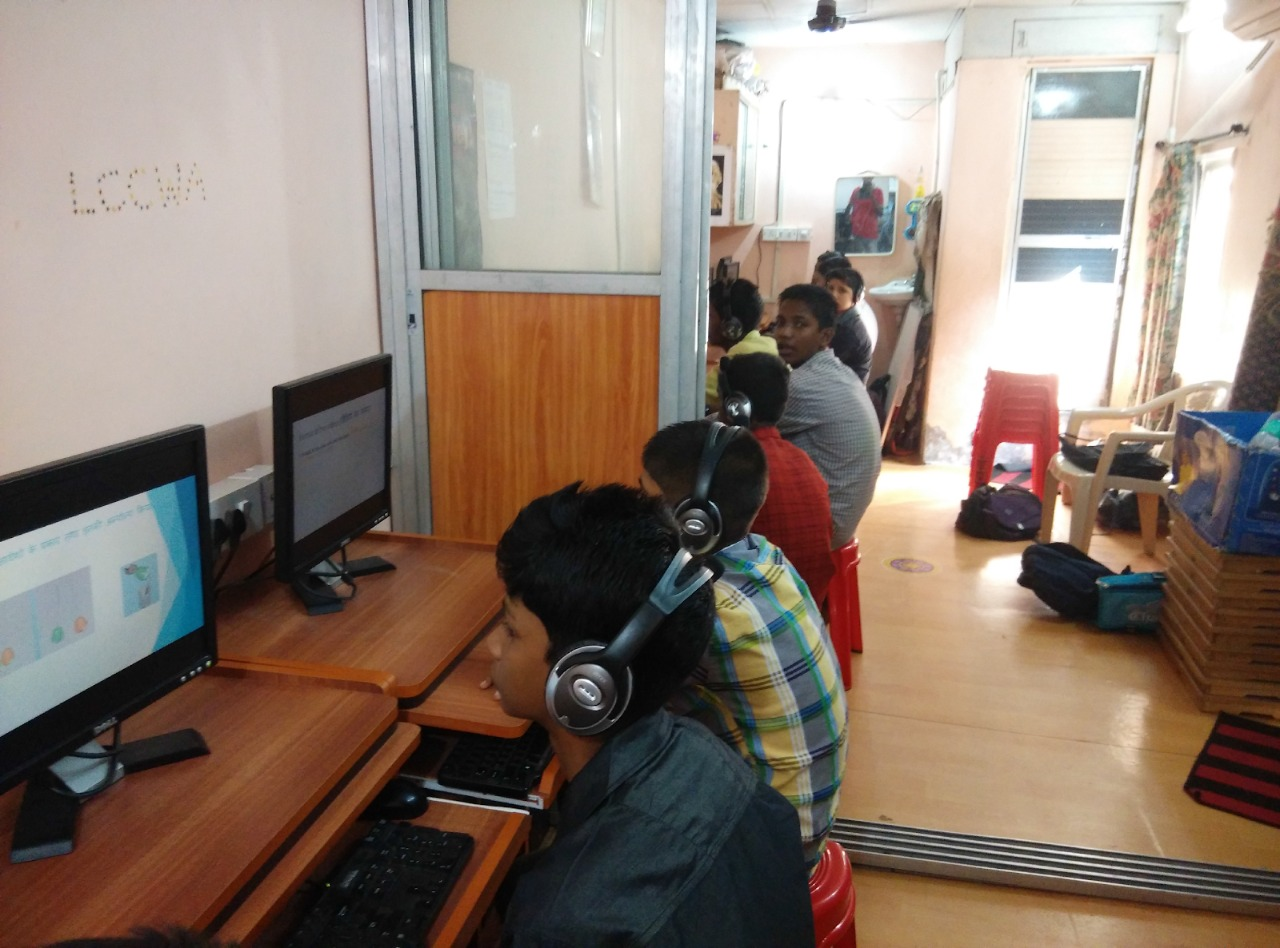
\includegraphics[width = 0.6\textwidth]{5.png}
% \caption*{Students of LCCWA NGO attending OLI sessions}
% \end{figure}

% \addcontentsline{toc}{subsection}{Teaching}
% \noindent \textbf{\Large Teaching:}\\ \\
% \noindent \textbf{About:} Teaching can be considered as the foundation stone of Educational Outreach. Our volunteers visit various NGOs in and around the campus to teach the students enrolled there. \\ \\
% \noindent \textbf{Outreach:}The NGOs currently involved with us are Vidya (having 5 centers), Asha, Logic Center and Community Welfare Association (LCCWA) and Computer Literacy Program (CLP) with 8 centers in all. A total of more than 70 volunteers taught more than 300 students in these centers. A continuous assessment program was carried out in NGOs by the implementation of log books to keep a record of every student’s academic growth. The teaching program was carried out in summer and winter vacations also with the aid of non-freshmen volunteers. 2 NGOs were functional with 20+ volunteers teaching a variety of subjects.
%  \\ \\
% \textbf{The way forward:}We plan to extend our volunteering to more NGOs in near future (distance of the NGO from the campus is a major constraint in this direction). Strengthening the ties between NGOs and NSS will also be focused on by helping out the NGOs with planning their summer camps and youth fests successfully.  \\ \\
% \begin{figure}[H]
% \centering
% \begin{subfigure}{.5\textwidth}
%   \centering
%  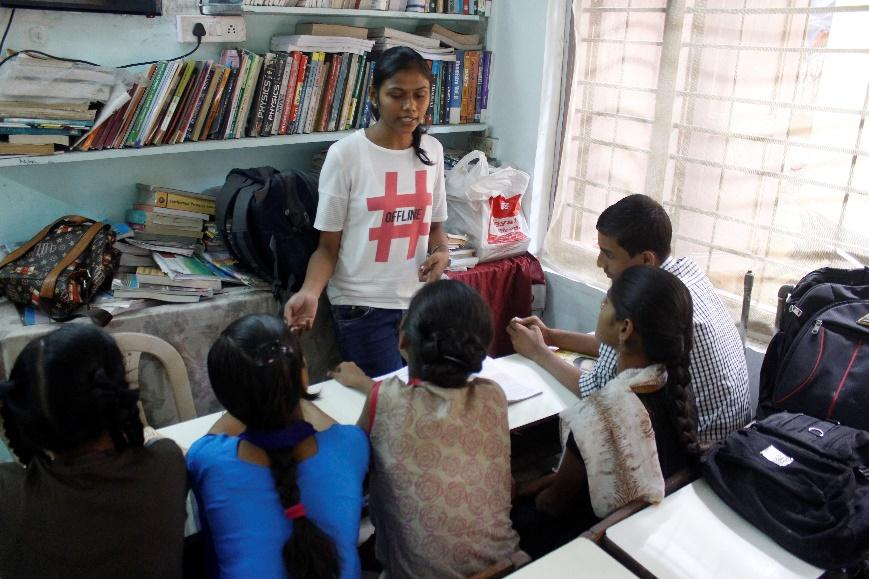
\includegraphics[width = 0.8\textwidth]{24.jpg}
% \end{subfigure}%
% \begin{subfigure}{.5\textwidth}
%  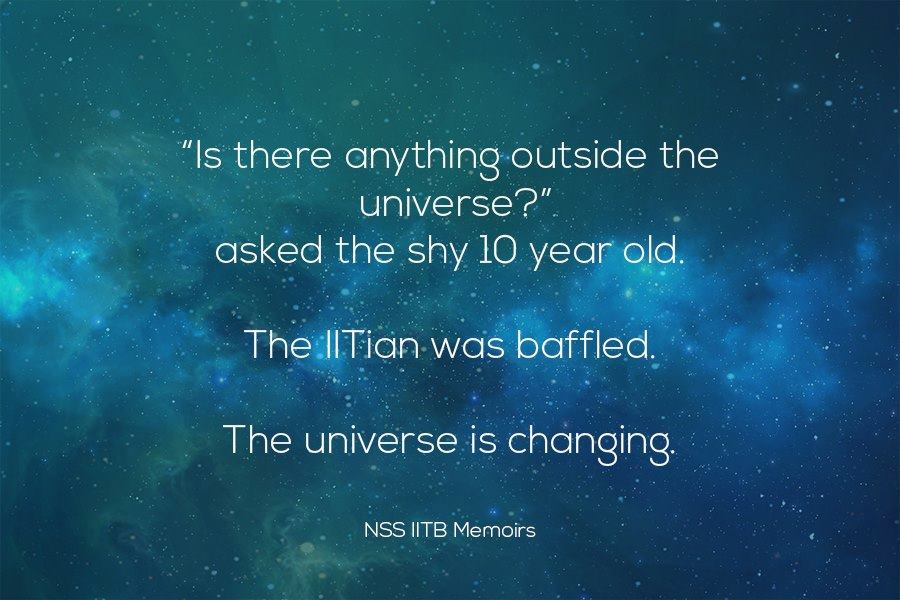
\includegraphics[width = 0.8\textwidth]{7.jpg}
% \end{subfigure}
% \caption*{Volunteers teaching in different NGOs}
% \end{figure}

% \addcontentsline{toc}{subsection}{Muskaan}
% \noindent \textbf{\Large Muskaan:}\\ \\
% \noindent \textbf{About:} Muskaan is a socio-cultural initiative which came to life by the joint efforts of NSS and the Institute Cultural Council. Muskaan was started with the aim of training children in cultural activities like dance and fine arts thus, contributing towards their all-round development. This year we incorporated a well-defined curriculum in all genres to ensure a robust learning experience. Quilling, origami, cotton-painting and blow-painting were some of the fine arts activities while bolly-hop and hip-hop were the major dance forms taught in the last year. Their efforts were showcased through a dance performance for All NSS Meet and through a fine arts submission for Kaladarshan 2018. Muskaan sessions are held every Sunday. We also had non-freshmen volunteers participating in this initiative over the course of two semesters.
% \\ \\

% \noindent \textbf{Outreach:} Over 100 students from 3 NGOs benefited from Muskaan \\

% \noindent \textbf{The Way Forward:} It has been planned to expand Muskaan to music and literary arts. Also, we aim at reaching out to more NGOs in near future. Better collaboration with the Institute Cultural Council and hence increased productivity in genres like Dramatics will be sought for.\\

% \begin{figure}[H]
% \centering
% \begin{subfigure}{.5\textwidth}
%  \centering
%  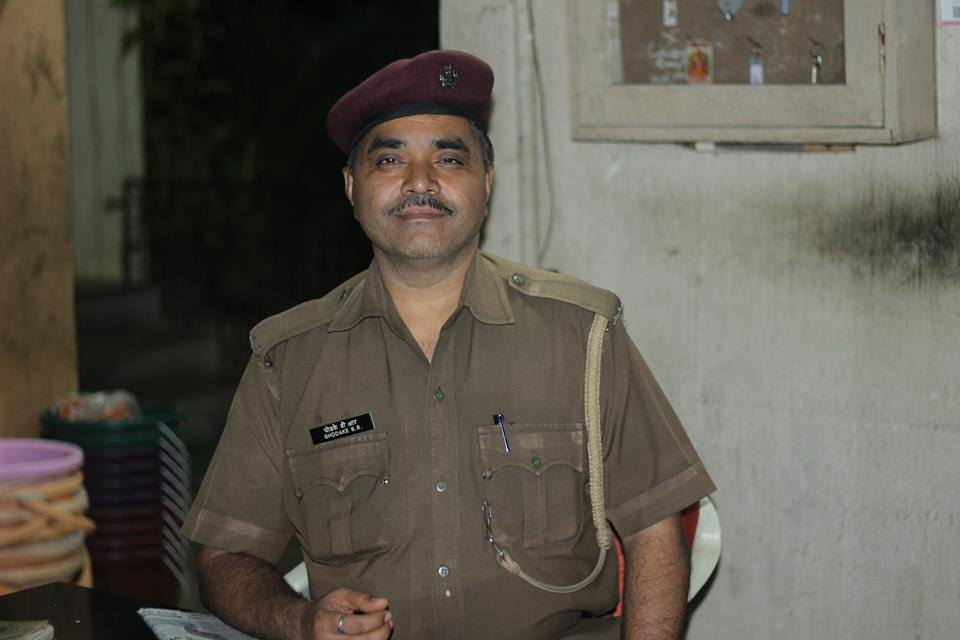
\includegraphics[width = 0.7\textwidth]{8.jpg}
% \end{subfigure}%
% \begin{subfigure}{.5\textwidth}
% 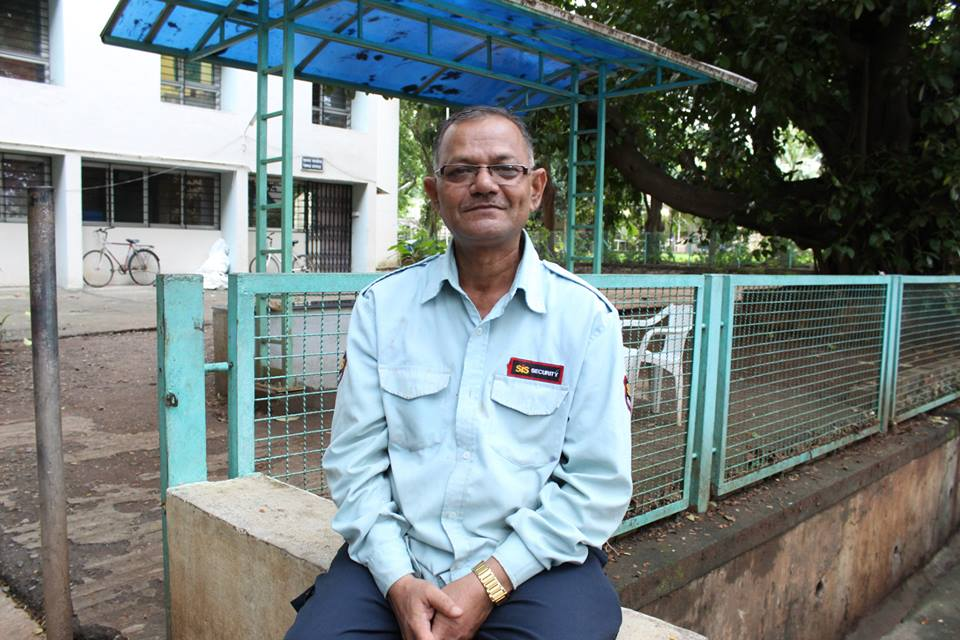
\includegraphics[width = 0.8\textwidth]{9.jpg}
% \end{subfigure}
% \caption*{Origami making session}
% \end{figure}

% \begin{figure}[H]
% \centering
% \begin{subfigure}{.5\textwidth}
%  \centering
%  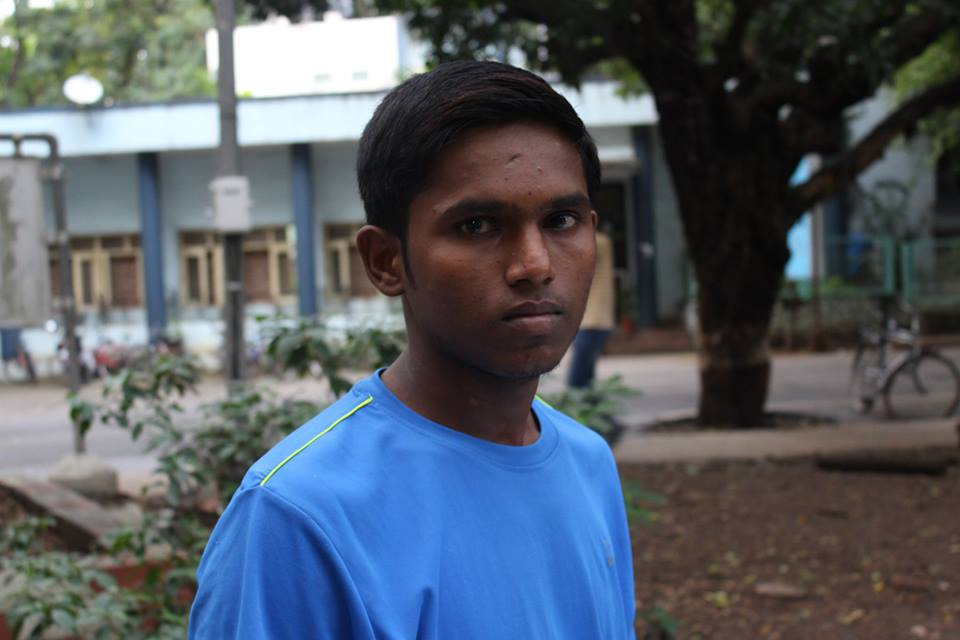
\includegraphics[width = 0.8\textwidth]{10.jpg}
% \end{subfigure}%
% \begin{subfigure}{.5\textwidth}
% 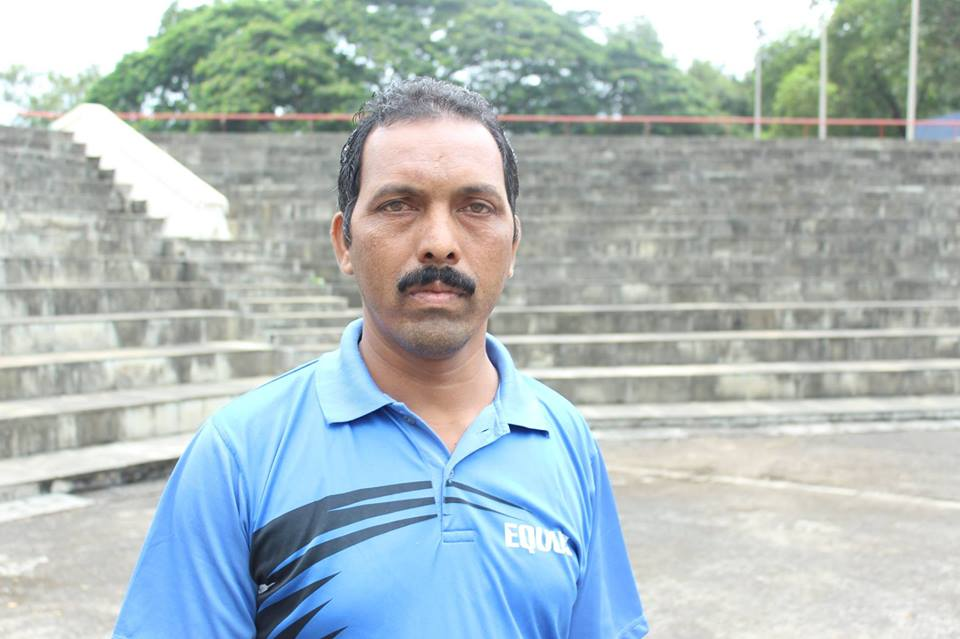
\includegraphics[width = 0.8\textwidth]{11.jpg}
% \end{subfigure}
% \caption*{Diya decoration session on the occasion of Diwali}
% \end{figure}

% \begin{figure}[H]
% \centering
% 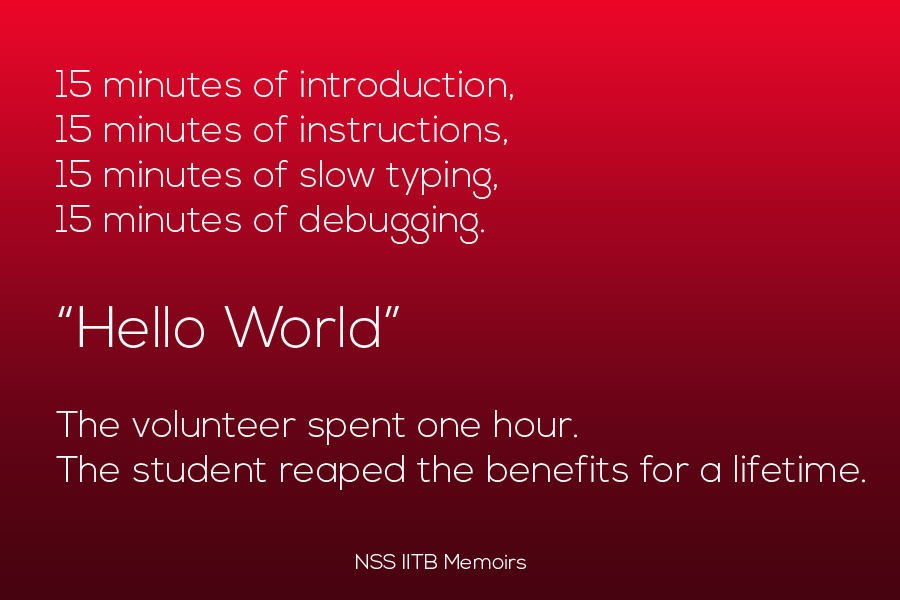
\includegraphics[width = 0.6\textwidth]{12.jpg}
% \caption*{Kaladarshan Artwork Entry by Muskaan kids}
% \end{figure}

% \begin{figure}[H]
% \centering
% 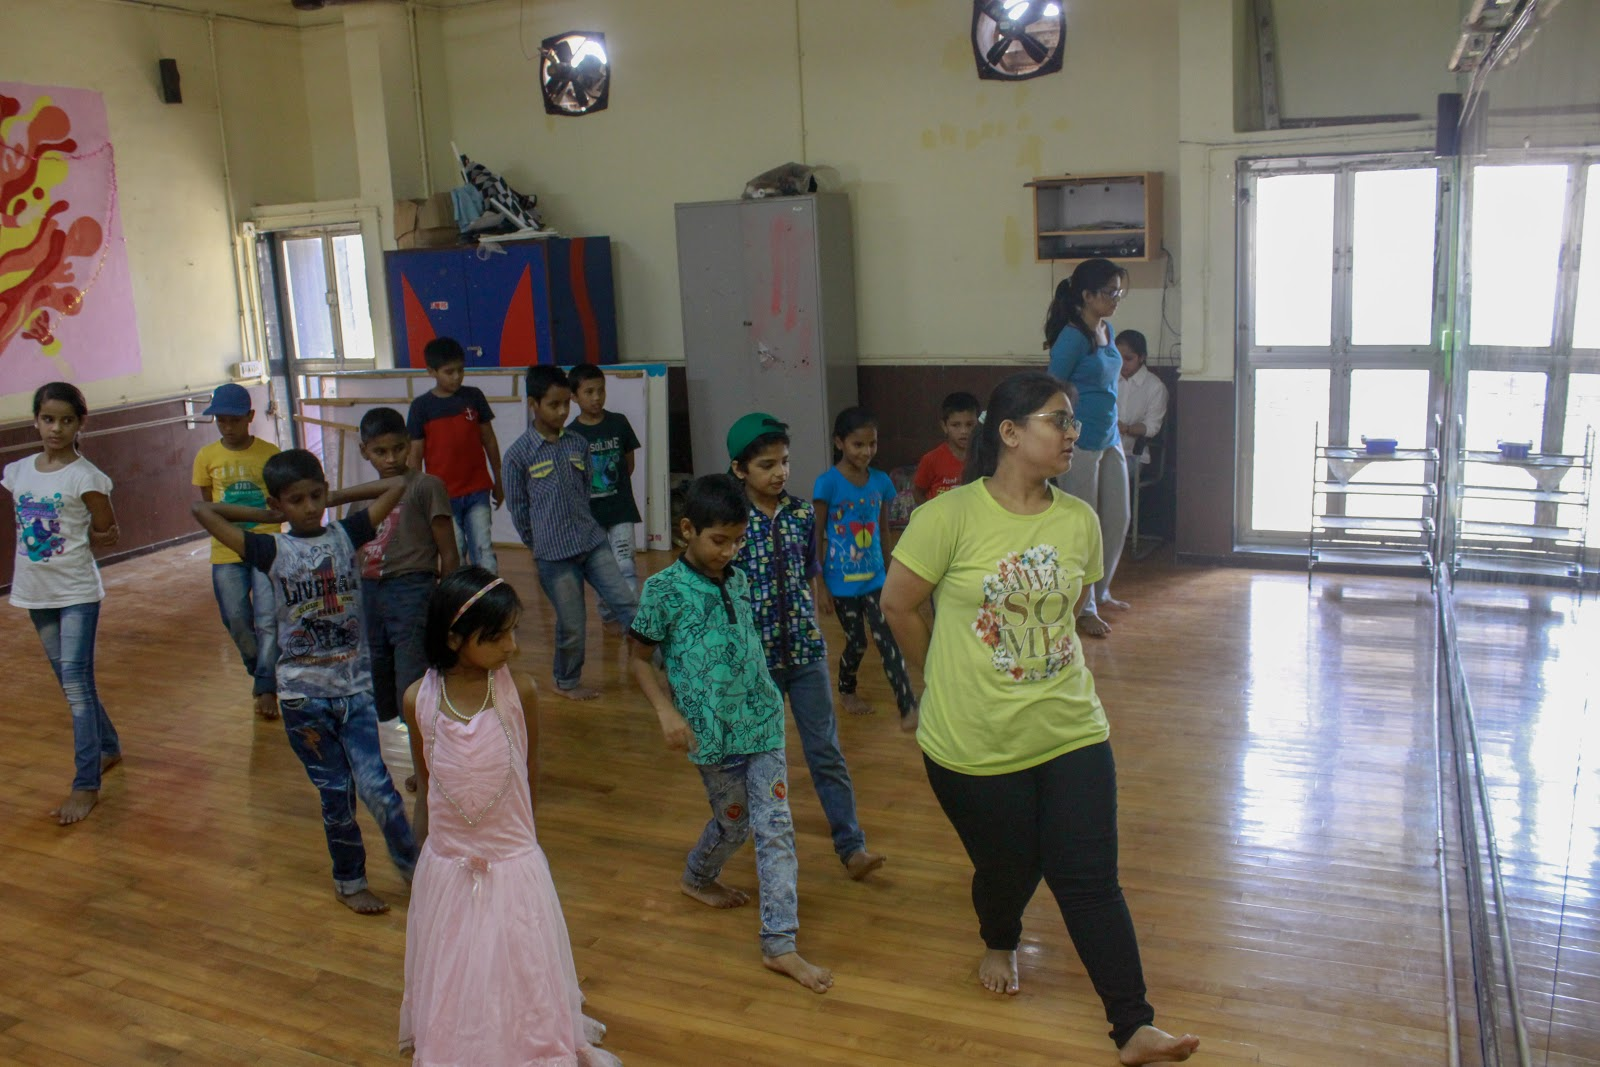
\includegraphics[width = 0.6\textwidth]{13.jpg}
% \caption*{Dance session}
% \end{figure}

% \addcontentsline{toc}{subsection}{Prayog}
% \noindent \textbf{\Large Prayog:}\\ \\
% \noindent “It vexes me when they would constrain science by the authority of the Scriptures, and yet do not consider themselves bound to answer reason and experiment.” – Galileo Galilei \\ \\
% Prayog was started with a belief that science is better understood by demonstration. Our aim is to instill scientific temperament among the students by the means of simple, yet interesting and informative scientific experiments. The students get a chance to perform the experiments themselves after the demonstration. Also, care is taken to ensure that the experiments are performed with readily available apparatus so that the students can easily replicate them when they go home. All the experiments are followed by an explanation of the scientific principles on which the experiment is based. We included mental ability section this time with quizzes and puzzles and fun activities. This year the students were also taken to various technical exhibitions inside the IIT campus to ignite their curiosity and inspire them towards science.
% \\

% \noindent \textbf{Outreach:} Over 100 students from 3 NGOs benefited from Prayog \\

% \noindent \textbf{The Way Forward:} We are trying to expand the experiment section on OLI channel by recording more Prayog experiments. Also, efforts are being made to introduce easily doable projects in Prayog. Experiment reports will also be incorporated shortly. Regular sessions will continue as before. \\

% \begin{figure}[H]
% \centering
% 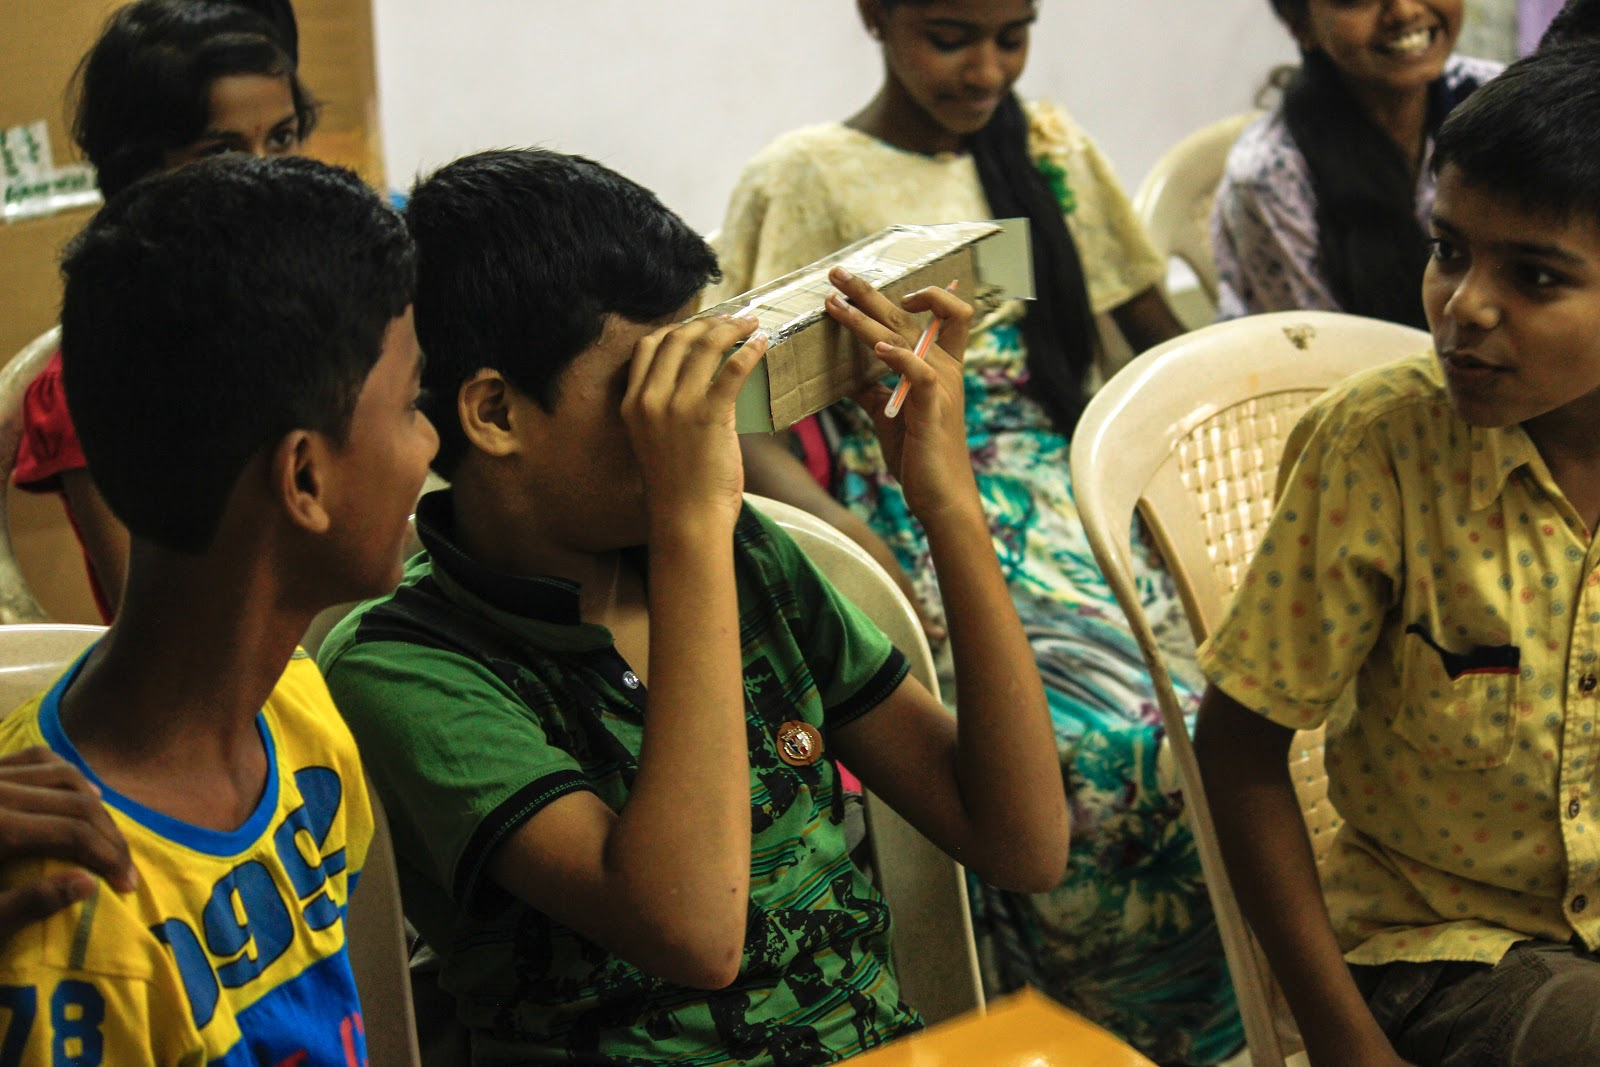
\includegraphics[width = 0.6\textwidth]{14.jpg}
% \end{figure}

% \begin{figure}[H]
% \centering
% \begin{subfigure}{.5\textwidth}
%  \centering
%  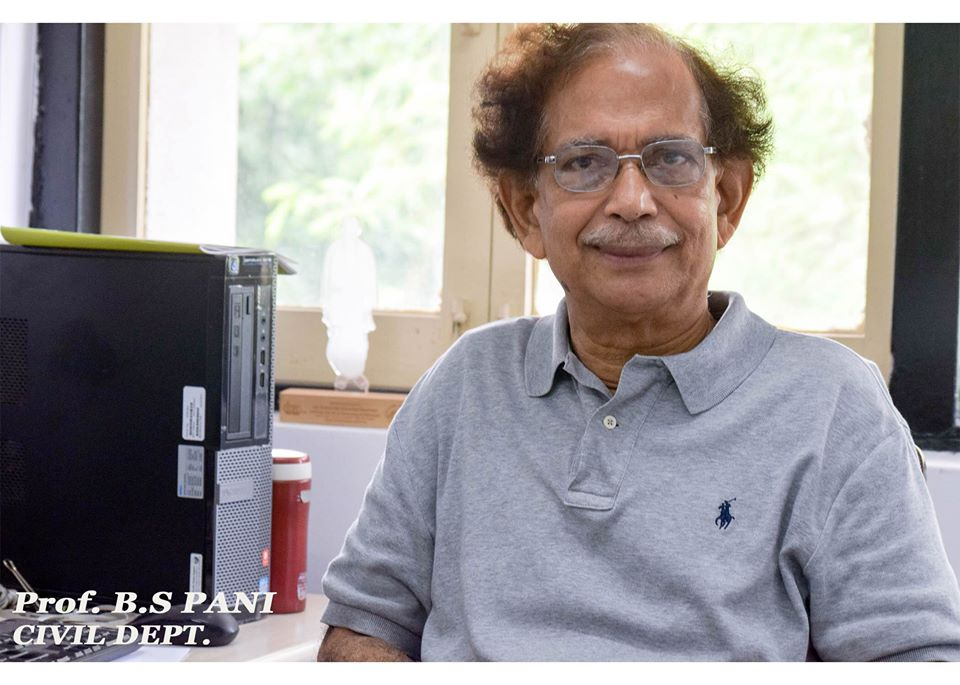
\includegraphics[width = 0.8\textwidth]{15.jpg}
% \end{subfigure}%
% \begin{subfigure}{.5\textwidth}
% 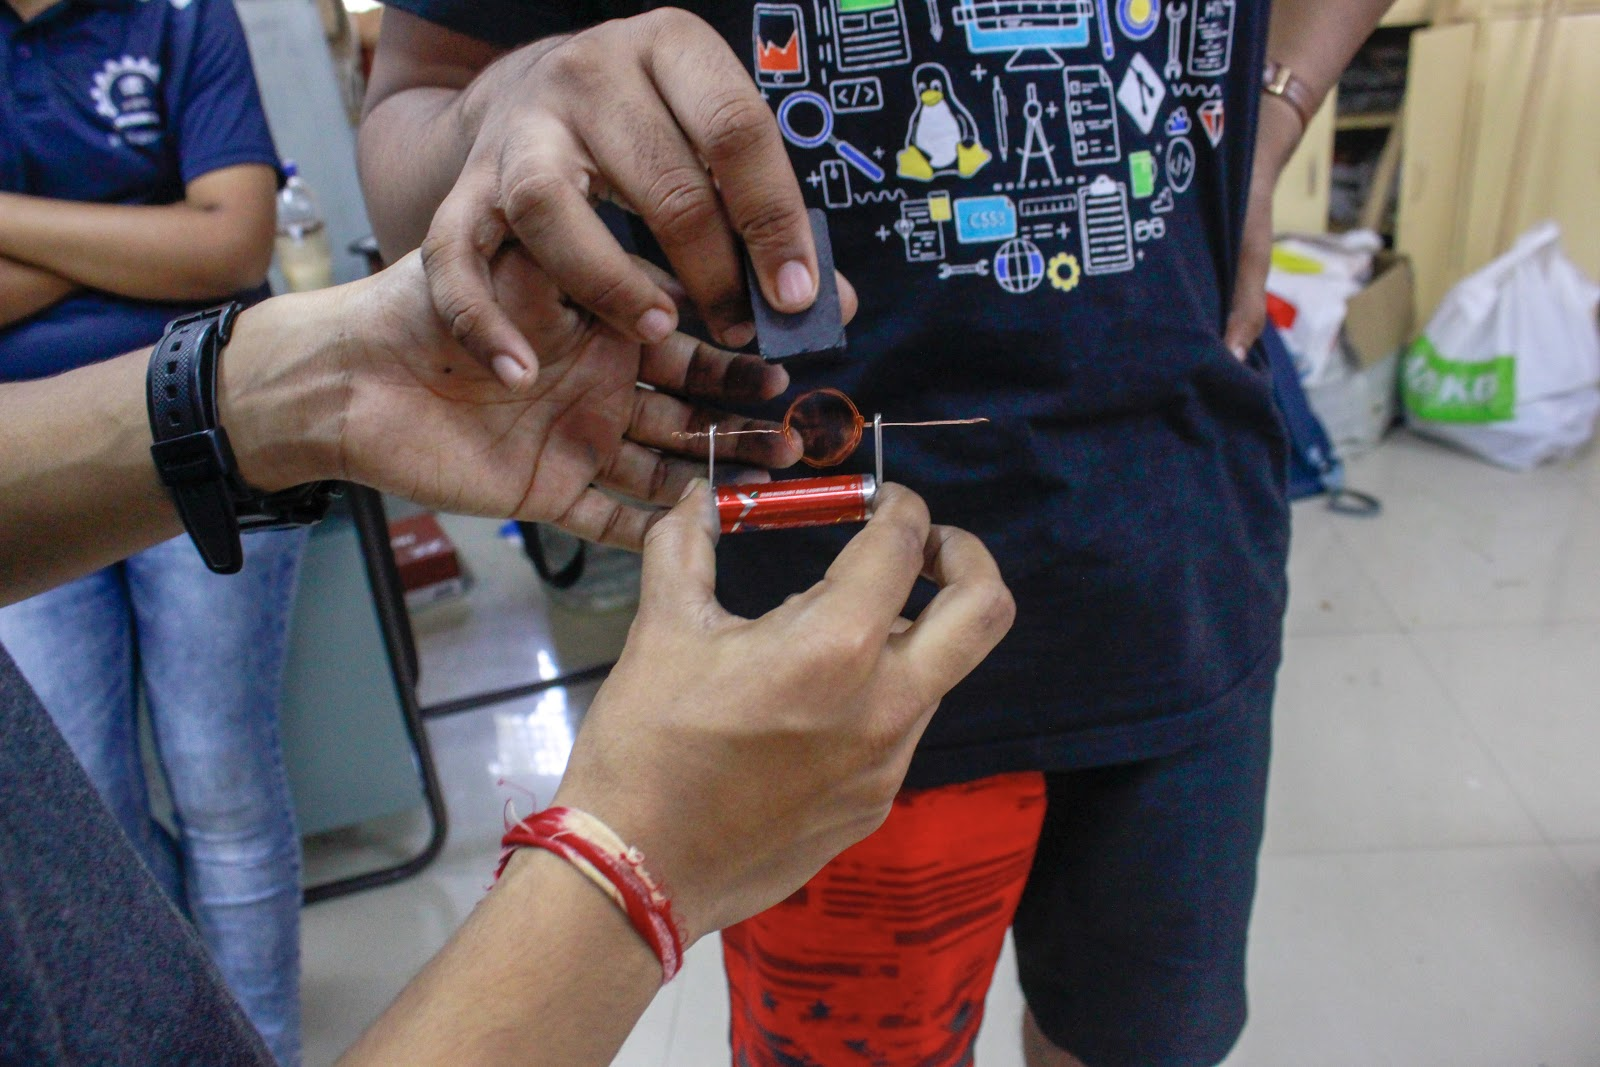
\includegraphics[width = 0.8\textwidth]{16.jpg}
% \end{subfigure}
% \caption*{Various experiments being performed and explained by volunteers}
% \end{figure}


% \noindent \textbf{\Large Voice For Purpose (VFP):}
% \addcontentsline{toc}{subsection}{Voice For Purpose (VFP)} \\ \\ \noindent \textbf{About the initiative:} Voice for Purpose is an initiative aimed at providing quality audiobooks for the visually impaired community via our YouTube channel which has increased the accessibility of these audiobooks and facilitate their distribution. We are currently focusing on providing literature ( both Hindi and English), and have launched new genres like Travel Diaries ( to provide picturesque descriptions of places which the visually impaired cannot see themselves) and Current Affairs ( with the aim to provide information about the world affairs). We also conducted a blind school visit where we had fun interaction with the kids. Requirements given by the blind school are being worked on.
% \\

% \noindent \textbf{Link: } \url{ https://www.youtube.com/channel/UC2iPnxGyKViqjV37f3r6uJw} \\
% \\ \noindent \textbf{The Way Forward:} The channel currently hosts 70+ audio recordings, has 200+ subscribers and 16k+ views. We plan on reaching out to blind foundations and schools and provide requested content.  Also, we plan on expanding our existing playlists with simultaneous creation of new ones.  \\

% \begin{figure}[H]
% \centering
% 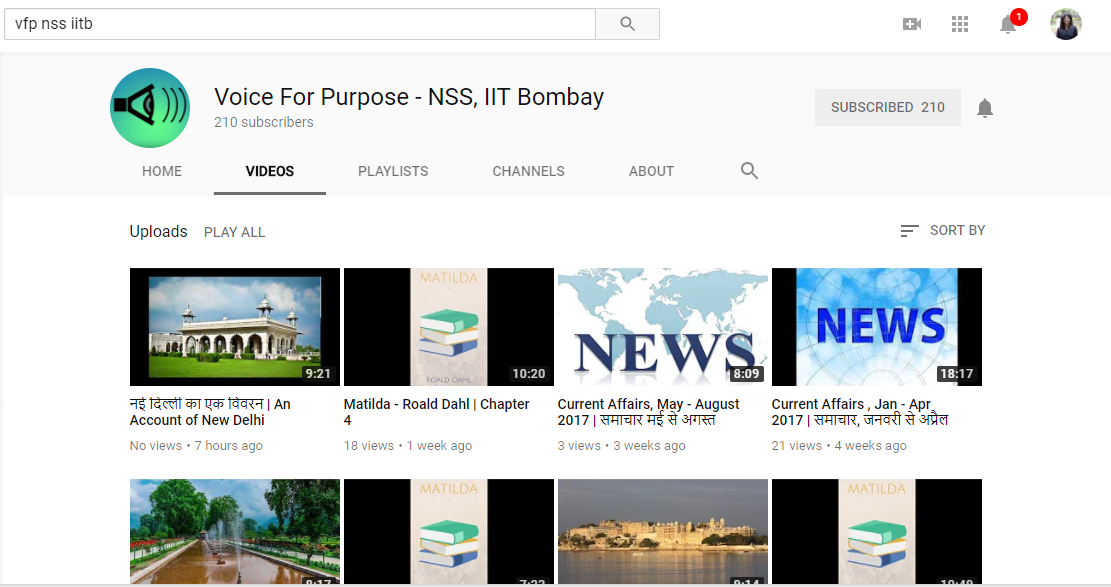
\includegraphics[width = 0.9\textwidth]{17.png}
% \caption*{YouTube channel for Voice For Purpose}
% \end{figure}

% \begin{figure}[H]
% \centering
% \begin{subfigure}{.5\textwidth}
%  \centering
%  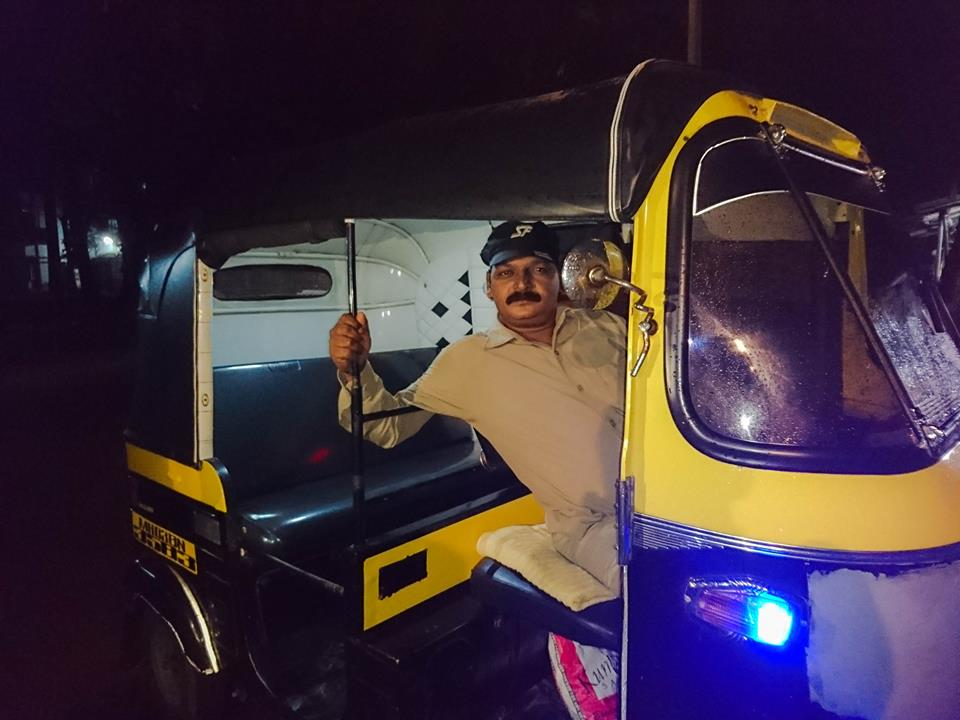
\includegraphics[width = 0.8\textwidth]{18.jpg}
% \end{subfigure}%
% \begin{subfigure}{.5\textwidth}
% 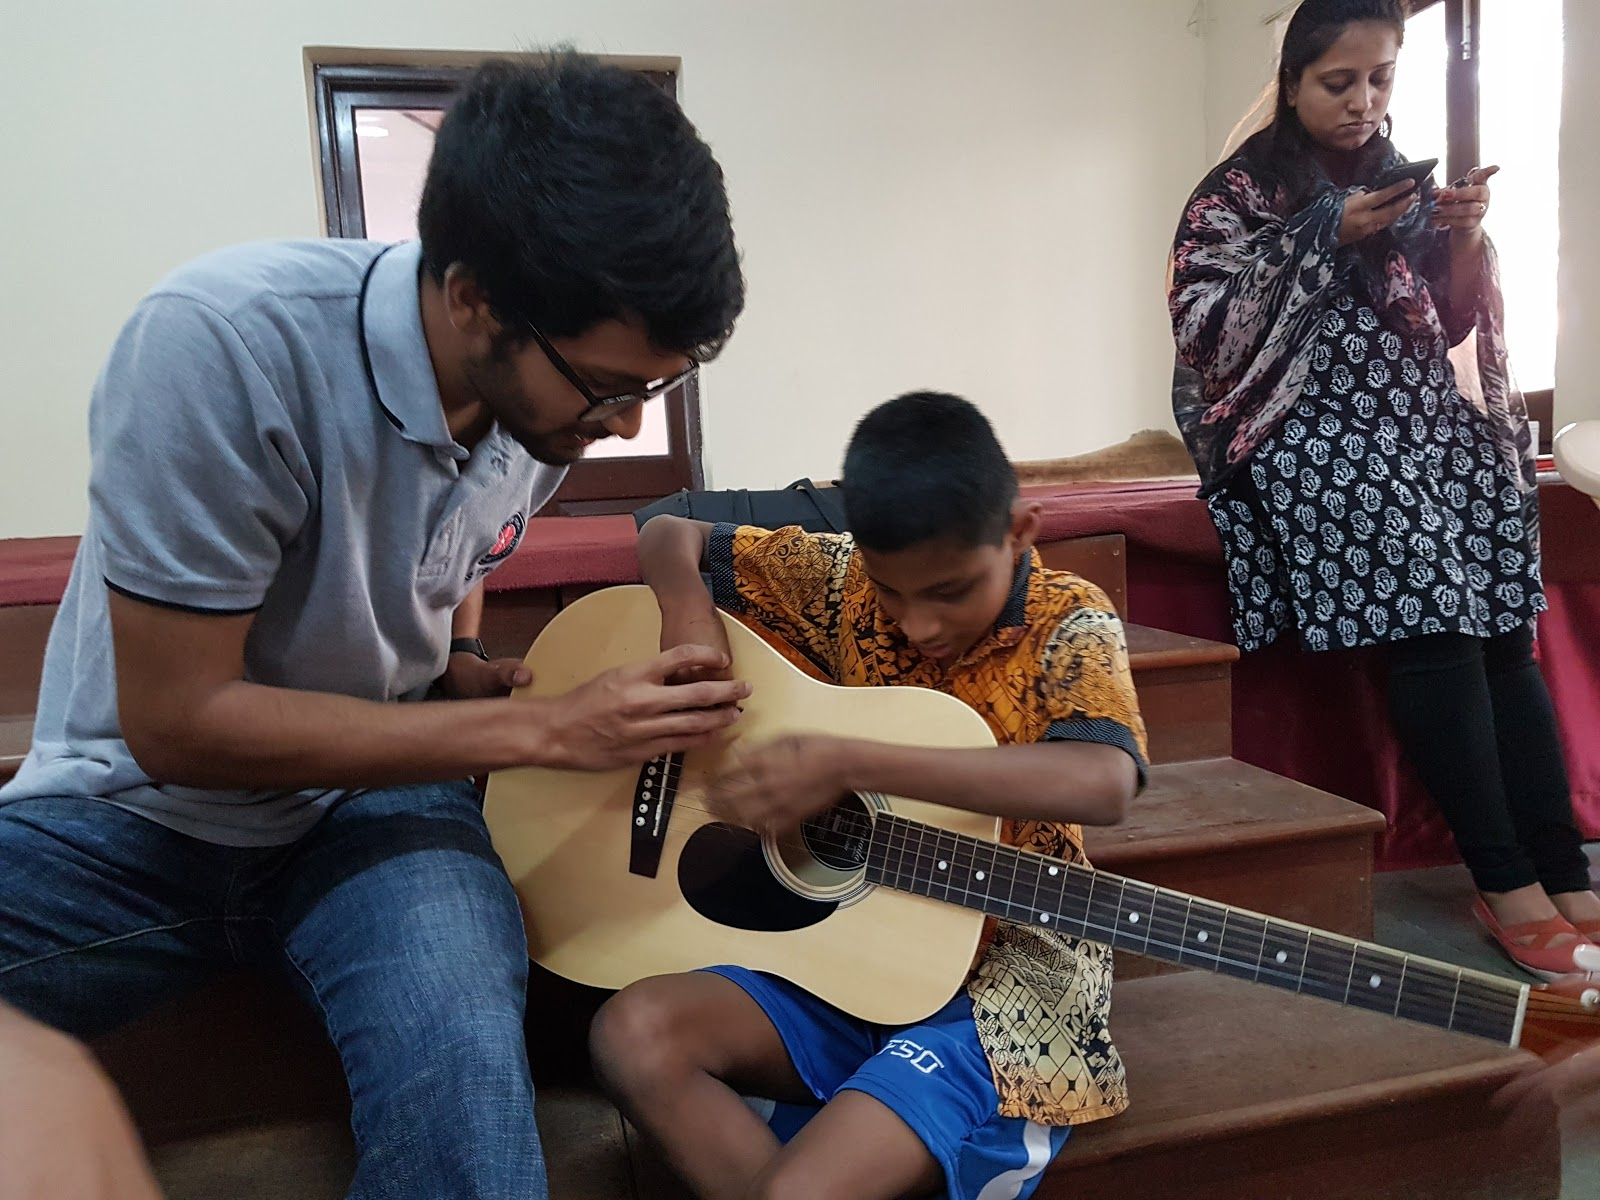
\includegraphics[width = 0.8\textwidth]{19.jpg}
% \end{subfigure}
% \caption*{Blind School Visit - Volunteers interacted with the kids with singing and story telling}
% \end{figure}

% \addcontentsline{toc}{subsection}{Adult Literacy Program}
% \noindent \textbf{\Large \linebreak Adult Literacy Program}\\ \\
% \noindent “Anyone who stops learning is old, whether at twenty or eighty. Anyone who keeps learning stays young.” ? Henry Ford
%  \\ \\This program was started on the request of security guards to teach them the basics of English. We have come a long way since then and ALP has been extended to mess workers. We have even expanded the curriculum to make it more relatable to the workers’ needs. We now have included basic mathematics and basic knowledge (going cashless, how to fill forms etc ) for the benefit of the workers. Currently, mess workers and PHO workers in Hostels – 2, 3, 6, 7, 8, 9, 10  are benefiting from this program. We distributed dictionaries and notebooks to the mess workers to facilitate their learning process. We have been receiving a very positive response for the program and the workers have shown commendable enthusiasm towards learning
% \\

% \noindent \textbf{Outreach:} Currently, 50+ mess workers from 7 hostels are a part of this program.\\
% \\
% \noindent \textbf{The Way Forward:} We plan on structuring ALP by making more robust and thorough teaching modules which will be modified with time. Also, expanding ALP to the rest of the hostels and possibly to construction workers will be the next move. \\

% \begin{figure}[H]
% \centering
% 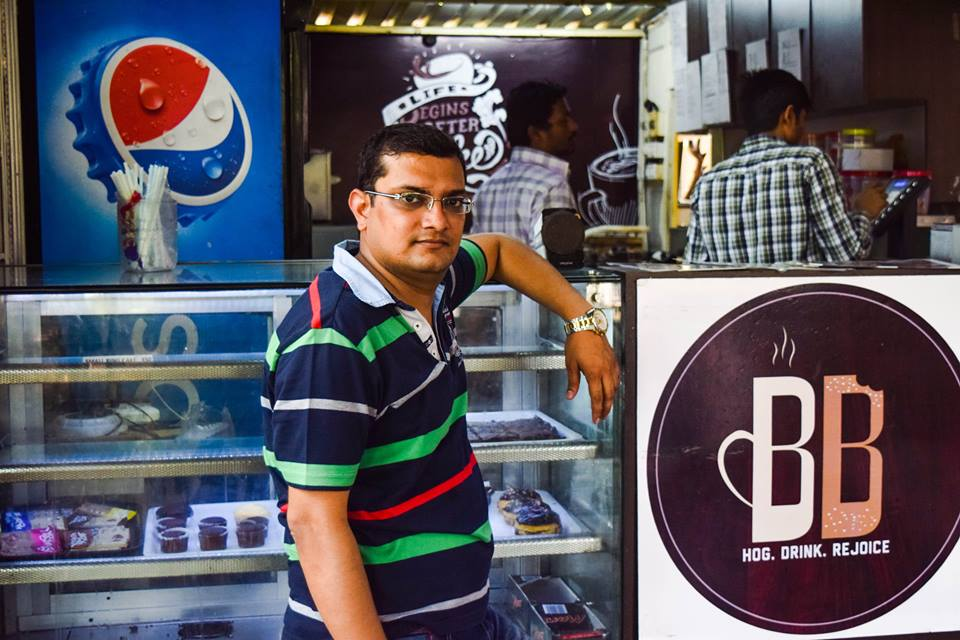
\includegraphics[width = 0.9\textwidth]{20.jpg}
% \end{figure}

% \begin{figure}[H]
% \centering
% 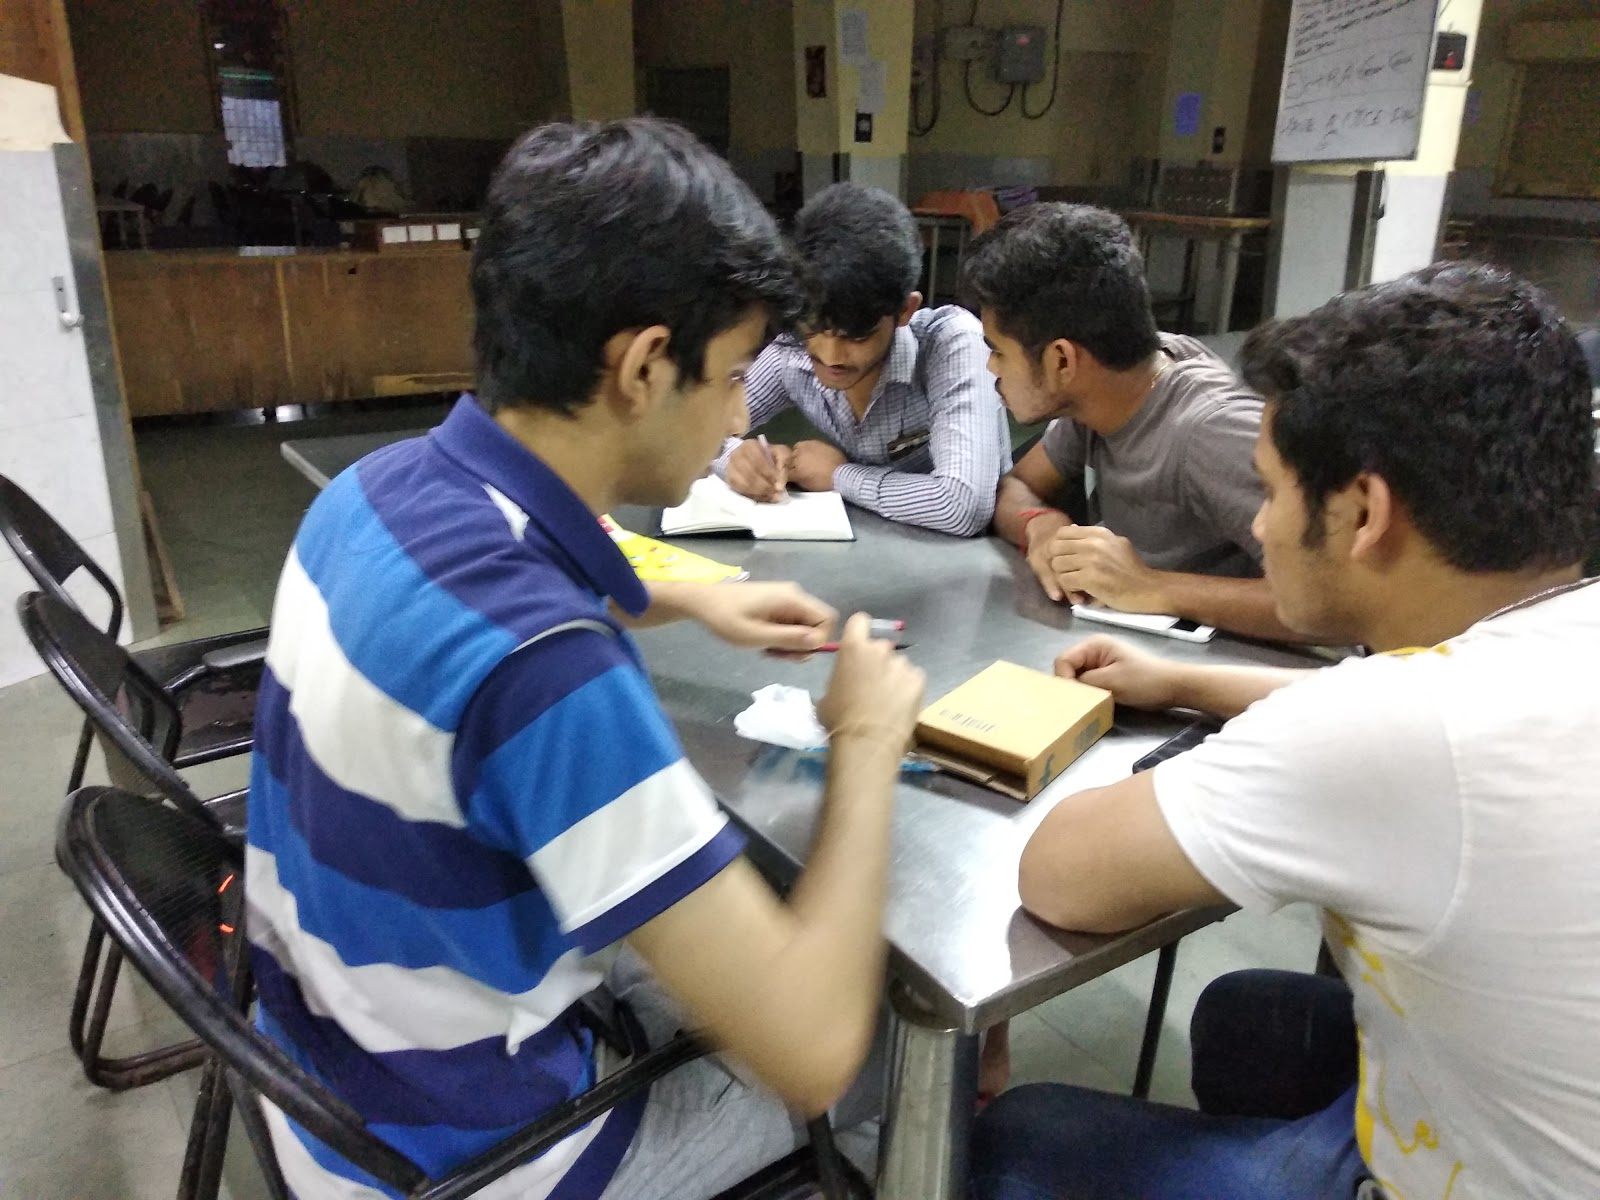
\includegraphics[width = 0.7\textwidth]{21.jpg}
% \caption*{ALP classes in different Hostels}
% \end{figure}

% \addcontentsline{toc}{subsection}{Neem Schools}
% \noindent \textbf{\Large \linebreak  \linebreak \linebreak \linebreak Neem Schools}\\ \\
% \noindent "Educating the mind without educating the heart is no education at all." - Aristotle
%  \\ \\While most schools do serve their purpose by educating the kids, somehow Value Education is something that is missed out. We were introduced to this idea by WhiteSwan Neem School foundation, a Delhi based organisation, who wanted to start neem schools in Mumbai. After proper induction and training, we took this initiative up. Currently we are functioning in Gokhale Nagar Maidan (opposite IIT Main Gate) and have 40+ children from around the slums attending these Sunday morning sessions. Every session starts with a prayer, followed by instructions for proper hygiene maintenance which then is followed by the session on moral value of the day. Interesting stories and interactive activities are used to get the moral message to the kids and at last the session ends with a prayer. Many a times parents of the kids come by to see the sessions progressing and give feedback to improve the sessions.
% \\

% \noindent \textbf{The Way Forward:} Expanding the Neem Schools to Phulenagar slum area ( to the left of Y Point gate) and starting these sessions in collaboration with NGOs operating in the areas will be the next step for Neem Schools.
%  \\

% \begin{figure}[H]
% \centering
% 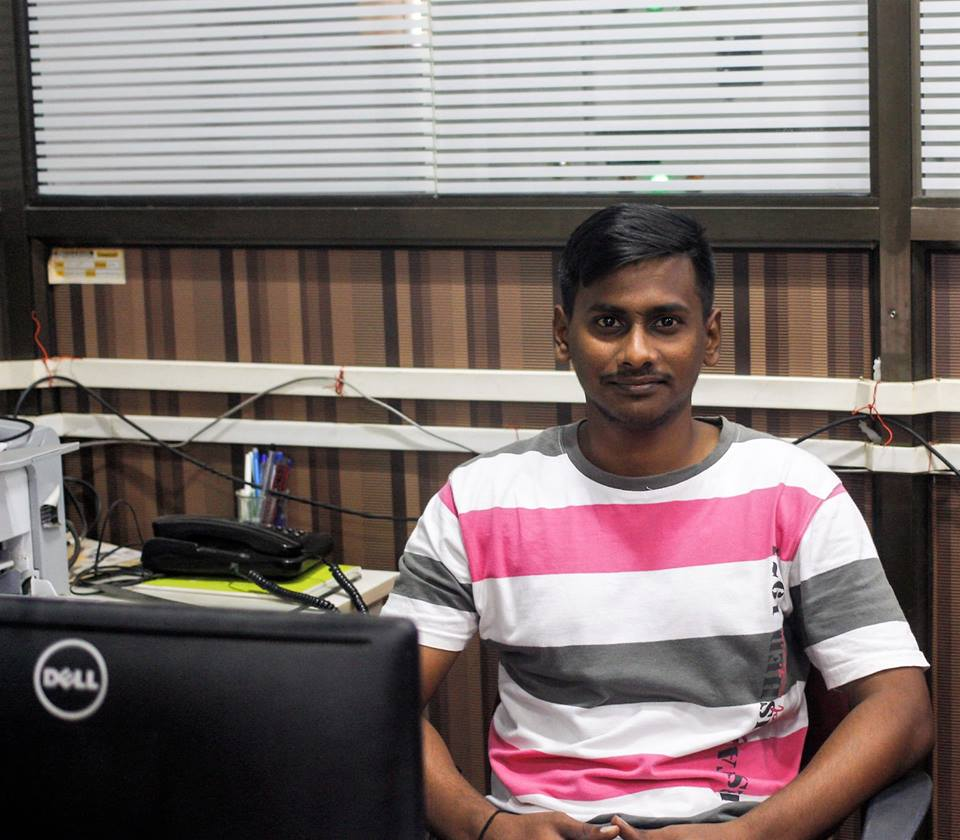
\includegraphics[width = 0.55\textwidth]{22.jpg}
% \caption*{Kids attending a Neem School session}
% \end{figure}

% \begin{figure}[H]
% \centering
% 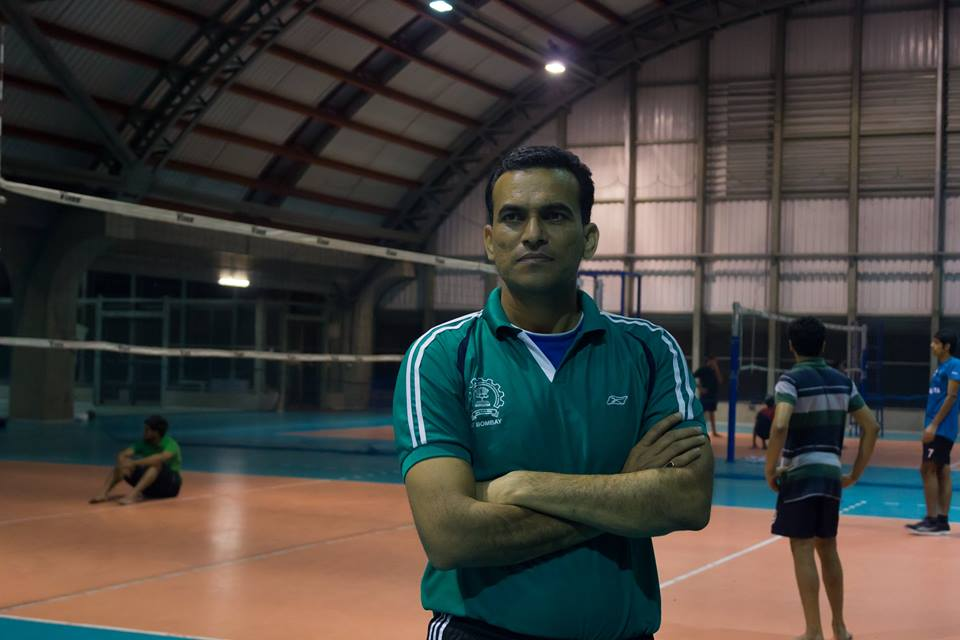
\includegraphics[width = 0.55\textwidth]{23.jpg}
% \caption*{Using videos to explain moral values and making the teaching interesting and effective}
% \end{figure}

% \pagebreak
% \chapter*{Green Campus}
% \markboth{Green Campus}{Green Campus}
% \addcontentsline{toc}{chapter}{Green Campus}

% \begin{figure}[H]
% \centering
% \hspace*{-2.3cm}
% \vspace*{-2.5cm}
% %\includegraphics[width = 1.26\textwidth]{Figures/GC.png}
% %\caption*{A snapshot of a game based on chemistry}
% \end{figure}

% \vspace*{-0.2cm}
% \addcontentsline{toc}{section}{About the Department}
% \section*{\LARGE About the Department:} Green Campus is the department which attempts to take people closer to nature and works in direction of establishing a relationship with it. While doing this, we try to serve the mother nature by building a sustainable ecosystem inside the institute. We conduct Plantation Drives, Sapling Collection Drives, Biodiversity Mapping thereby making the volunteers feel the ecstasy of being in close relation with nature.

% \addcontentsline{toc}{section}{ Activities}
% \section*{\LARGE Major Activities}

% \addcontentsline{toc}{subsection}{Sapling Collection Drive:}
% \noindent \textbf{\Large Sapling Collection Drive:}\\ \\Every monsoon, many small saplings self-germinate near there large parent tree which later perishes due to insufficient sunlight and competition for nutrition as they are closely placed. So the volunteers collected these saplings transplanted them in covers and nurtured in the NSS nursery. When the saplings became self sustainable they were planted in hostels and different parts of the institute.This year we collected more than 200 saplings of Jamun, Mango, Jungli Badam, Taad, Umber etc.\\

% \begin{figure}[H]
% \centering
% 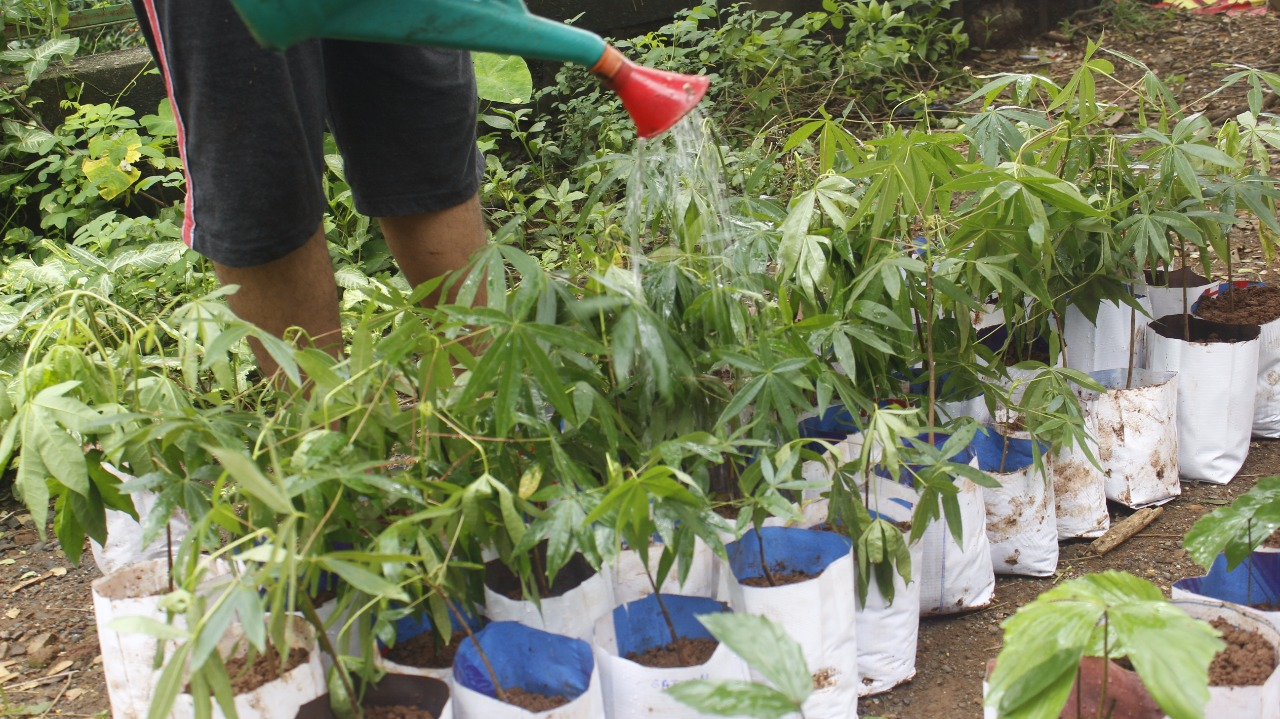
\includegraphics[width = 0.9\textwidth]{g1.JPG}
% \caption*{Saplings of Jungli Badam that were collected in the drive}
% \end{figure}

% \addcontentsline{toc}{subsection}{Hostel Plantation and Workshop:}
% \noindent \textbf{\Large Hostel Plantation and Workshop:}\\ \\To specifically involve more students in plantation, we started conducting sessions in hostels.Plantation workshops were organized in Hostel 2, 4, 5, 6, 7, 9, 14, 15 and 16.  Hostel inmates were also involved in the workshop where they reused waste plastic bottles to plant saplings which were used to decorate the corridors. Mostly these plantations were done during hostel fests, Republic day and Independence day.Some of the hostels councils also approached us for help in the development of their gardens.\\

% \begin{figure}[H]
% \centering
% 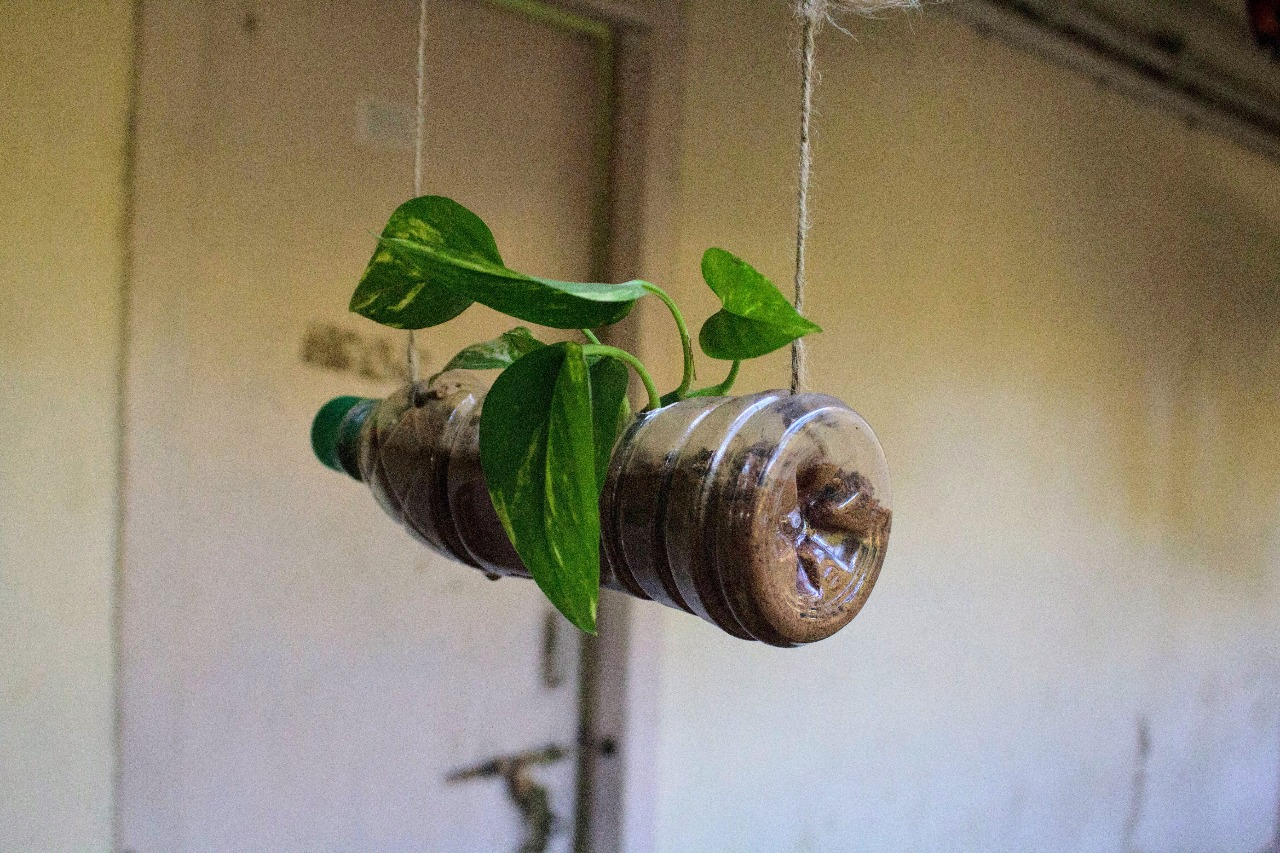
\includegraphics[width = 0.9\textwidth]{g2.jpg}
% \caption*{Money plant hanging in a hostel corridor}
% \end{figure}

% \addcontentsline{toc}{subsection}{Flex Cover Making:}
% \noindent \textbf{\Large Flex Cover Making:}\\ \\The conventional black plastic covers used for planting seeds and saplings in the NSS nursery were replaced by the covers which were made by waste flexes used for advertisements during fests and other institute events. The volunteers made covers of various sizes. This is one of our new activity promoting the concept of ‘Best out of Waste’.\\


% \begin{figure}[H]
% \centering
% \begin{subfigure}{.5\textwidth}
%  \centering
%  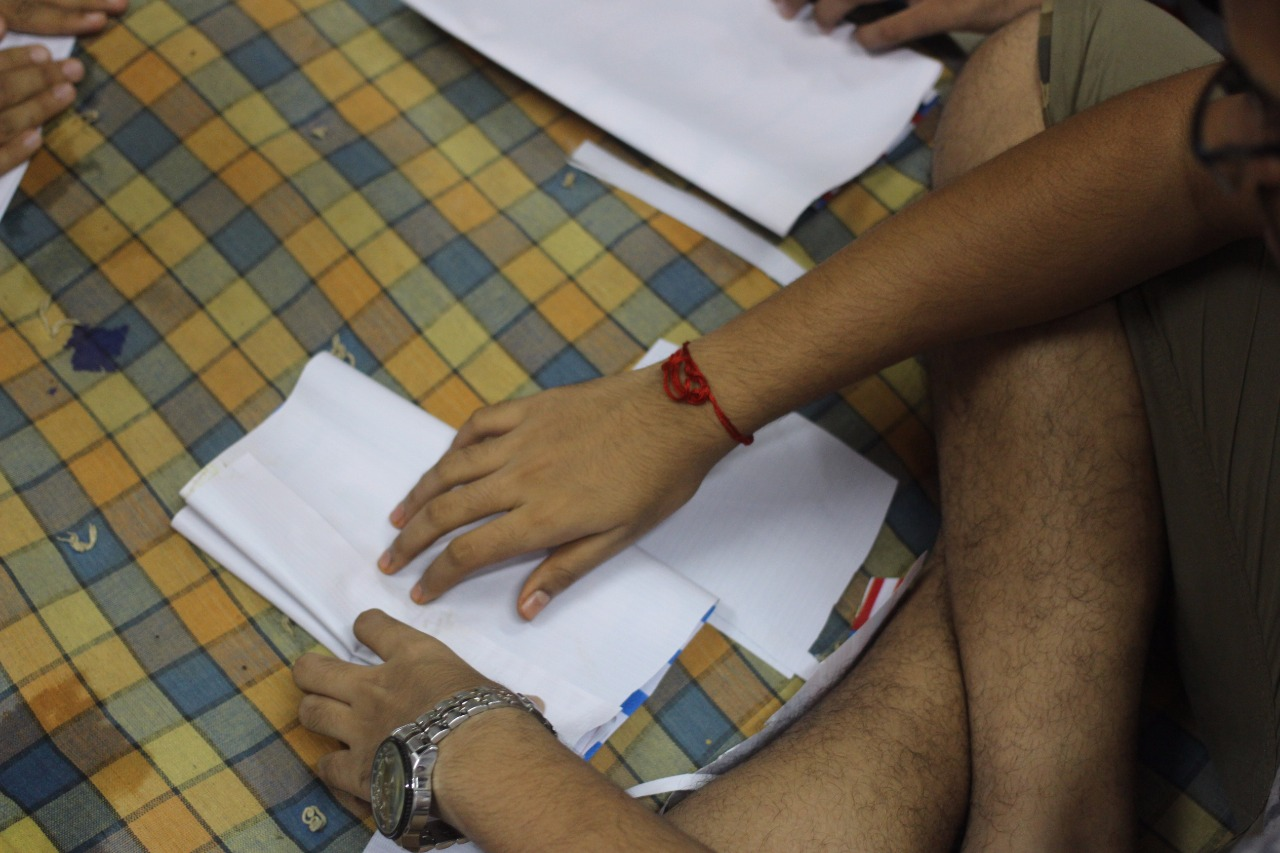
\includegraphics[width = 0.8\textwidth]{g3.JPG}
% \end{subfigure}%
% \begin{subfigure}{.5\textwidth}
% 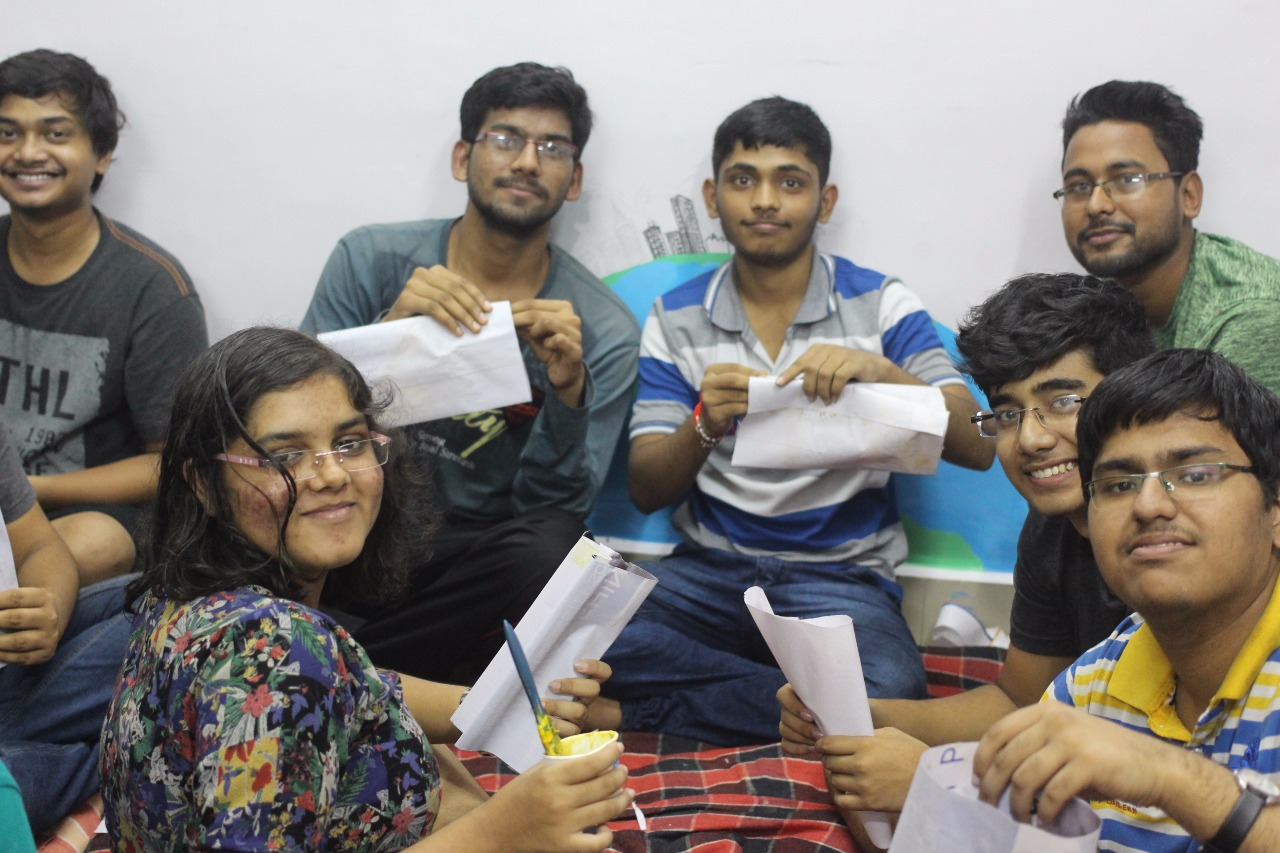
\includegraphics[width = 0.8\textwidth]{g4.JPG}
% \end{subfigure}
% \caption*{Volunteers making covers out of flexes}
% \end{figure}

% \addcontentsline{toc}{subsection}{Greenopedia:}
% \noindent \textbf{\Large Greenopedia:}\\ \\ An online portal where one can find all relevant information of various tree species present in the campus. Volunteers made small videos on each of the species which contained all interesting features of the tree. Apart from this the portal also contains the accessible locations of various trees in the institute. This portal is linked to the placards by QR codes on them which makes access to this portal simple. \\ \\

% \addcontentsline{toc}{subsection}{Biodiversity Mapping:}
% \noindent \textbf{\Large Biodiversity Mapping:}\\ \\Biodiversity mapping is the idea of locating the exact position of trees in given area and creating a database out of it. This is important in long term as it gives us the data trends of each species of the tree like which species are increasing or decreasing in number. This database can be created as per area. We can search for reasons of these data trends and take corrective measures if required. Student community in the campus have a huge set of activities which they can participate in and this causes them to pay very little attention to the huge biodiversity they pass by daily. We thought there can be an easy way of making this biodiversity data available to the community where they do not need to invest extra time to acquire it and praise the importance. So in addition to mapping the trees, we chose main road inside the campus and put the placards on trees bearing their names and specialty. Thus the information of biodiversity along the road is now made available to all the passers-by.
% \linebreak
% \linebreak
% We started the work by taking “Study of the Biodiversity of Indian Institute of Technology Bombay Campus” by WWF as the basic data. It was the data from 2008-09. We took the names of the trees from that report and made a database of their images with the help of volunteers. Later, we started identifying the trees in the main roadside. Volunteers also tried to explain the speciality of the tree through one liner info. Eventually, we put the common name, scientific name and speciality of the tree on the placard and put these placards on the trees. Care was taken so that no tree was harmed by the activity.
% \linebreak
% \linebreak
% This year in this initiative, to improvise, we used one sided paper for this activity which were collected from different departments and academic area. More than 1200 placards were labeled.  Also this time the placards were digitised by introduction of QR codes which when scanned redirects to Greenopedia (an online database).\\

% \begin{figure}[H]
% \centering
% 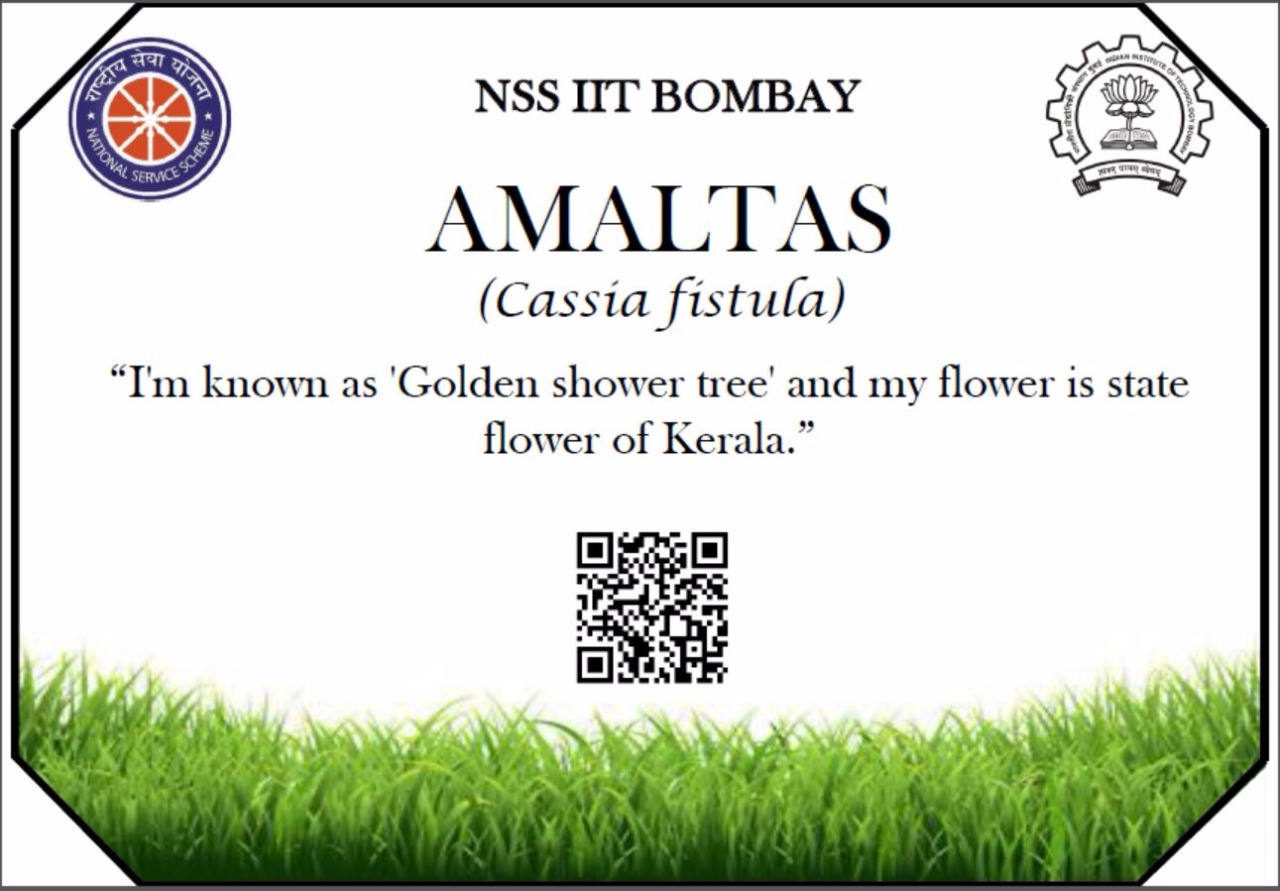
\includegraphics[width = 0.9\textwidth]{g12.JPG}
% \caption*{Sample placard used in biodiversity mapping}
% \end{figure}

% \begin{figure}[H]
% \centering
% \begin{subfigure}{.6\textwidth}
%  \centering
%  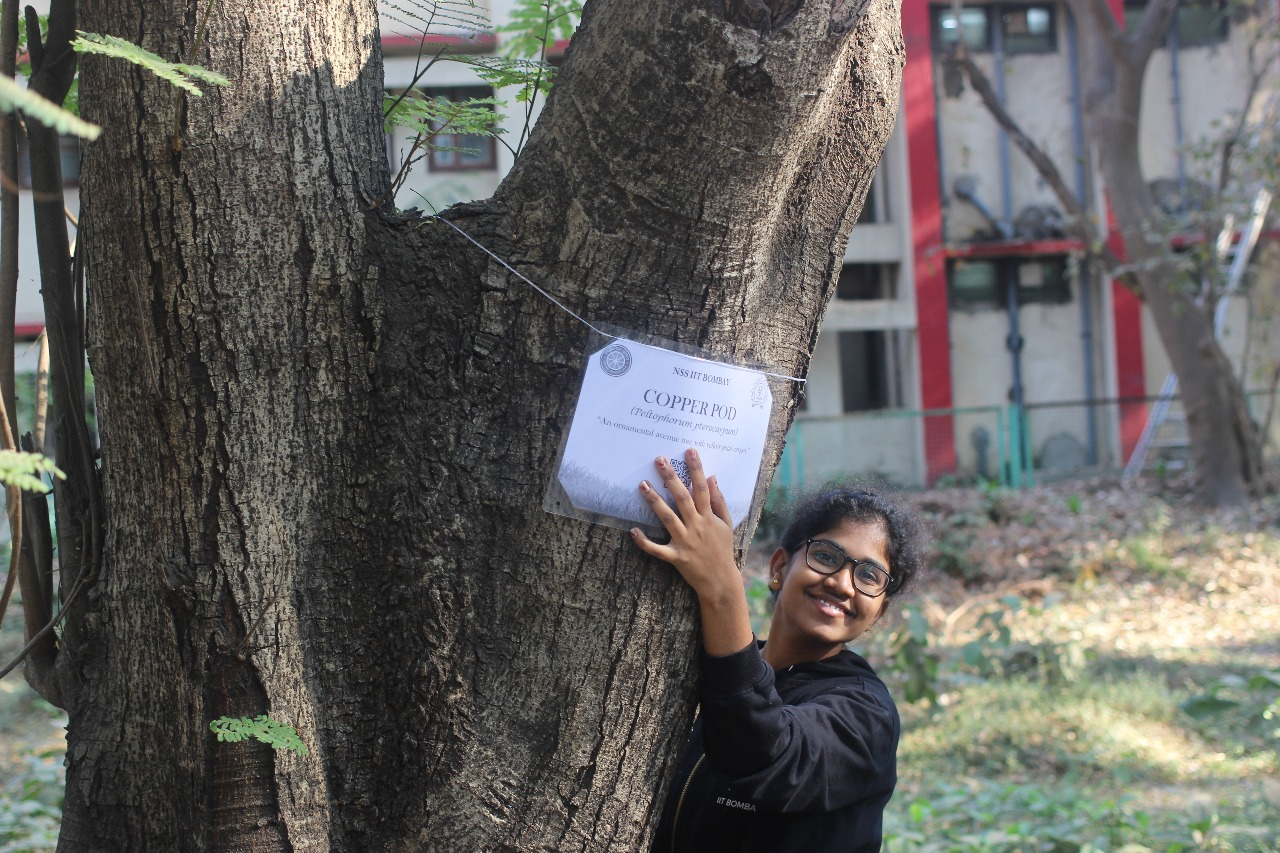
\includegraphics[width = 0.8\textwidth]{g5.JPG}
% \end{subfigure}%
% \begin{subfigure}{.6\textwidth}
% 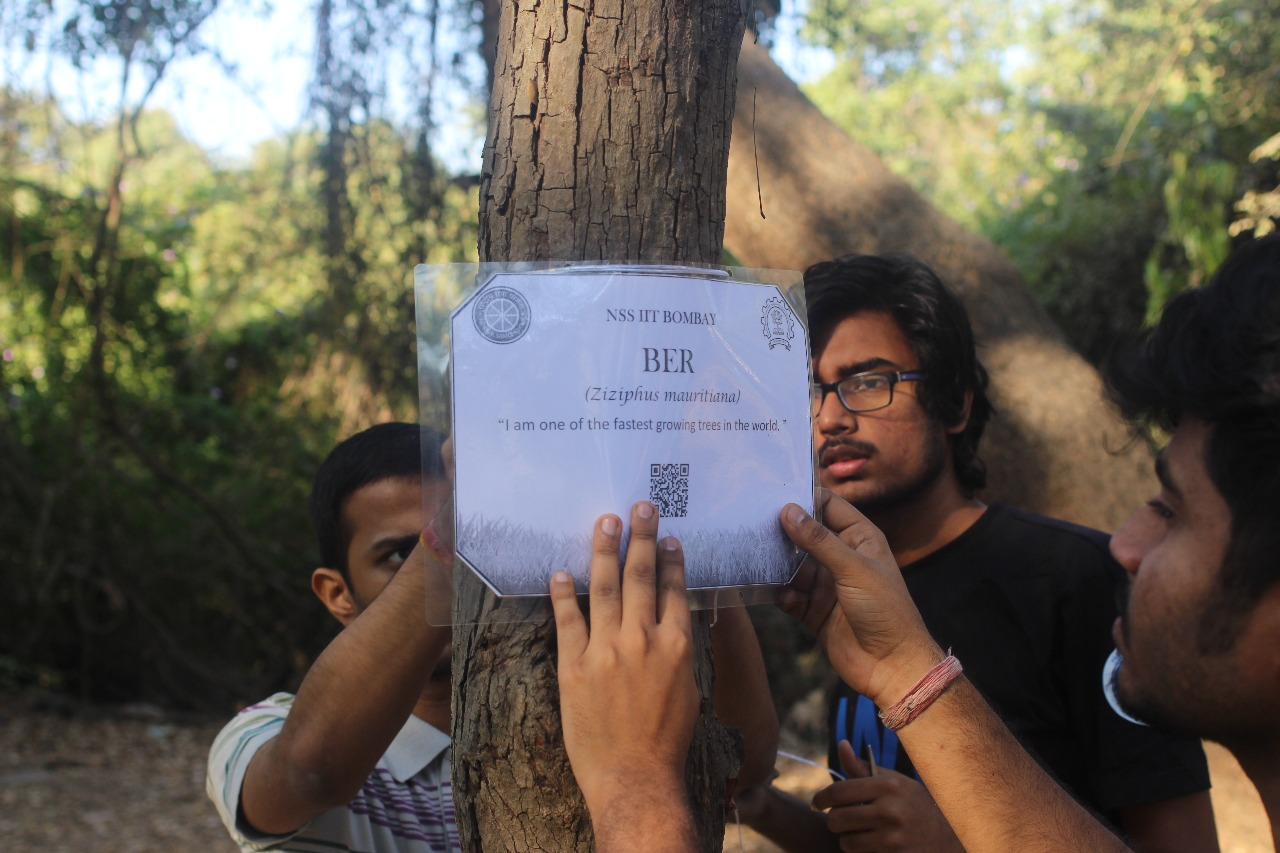
\includegraphics[width = 0.8\textwidth]{g6.JPG}
% \end{subfigure}
% \caption*{Volunteers tying Placards}
% \end{figure}

% \addcontentsline{toc}{subsection}{Bio-Composting:}
% \noindent \textbf{\Large \linebreak Bio-Composting:}\\ \\We used dry leaves collected by PHO (Public Health Office) workers from institute roads and hostel mess vegetable waste for making the compost manure. This served as the natural organic fertilizer for the plants, making the nursery self sustainable and at the same time facilitating the reuse of waste. We have been using this method of composting to convert the infertile soil in the triangular area outside the nursery into a fertile one.\\
% \linebreak
% \linebreak

% \addcontentsline{toc}{subsection}{Plantation in Coconuts:}
% \noindent \textbf{\Large Plantation in Coconuts:}\\ \\It is an unique way of plantation in which saplings were planted in the used coconut shells. Also when transplanted with the shell, the coconut degrades in the soil thereby providing nutrients. We collected more than 50 empty coconuts from the institute and planted Balsam saplings in them. In this process, we made holes in the bottom of the coconut, filled it with mud and planted the seeds or saplings in it. The holes in the coconut helped the roots to grow without any obstruction. This activity reduced the usage of the conventional black plastic covers in our Nursery thereby promoting sustainability.\\

% \begin{figure}[H]
% \centering
% \begin{subfigure}{.6\textwidth}
%  \centering
%  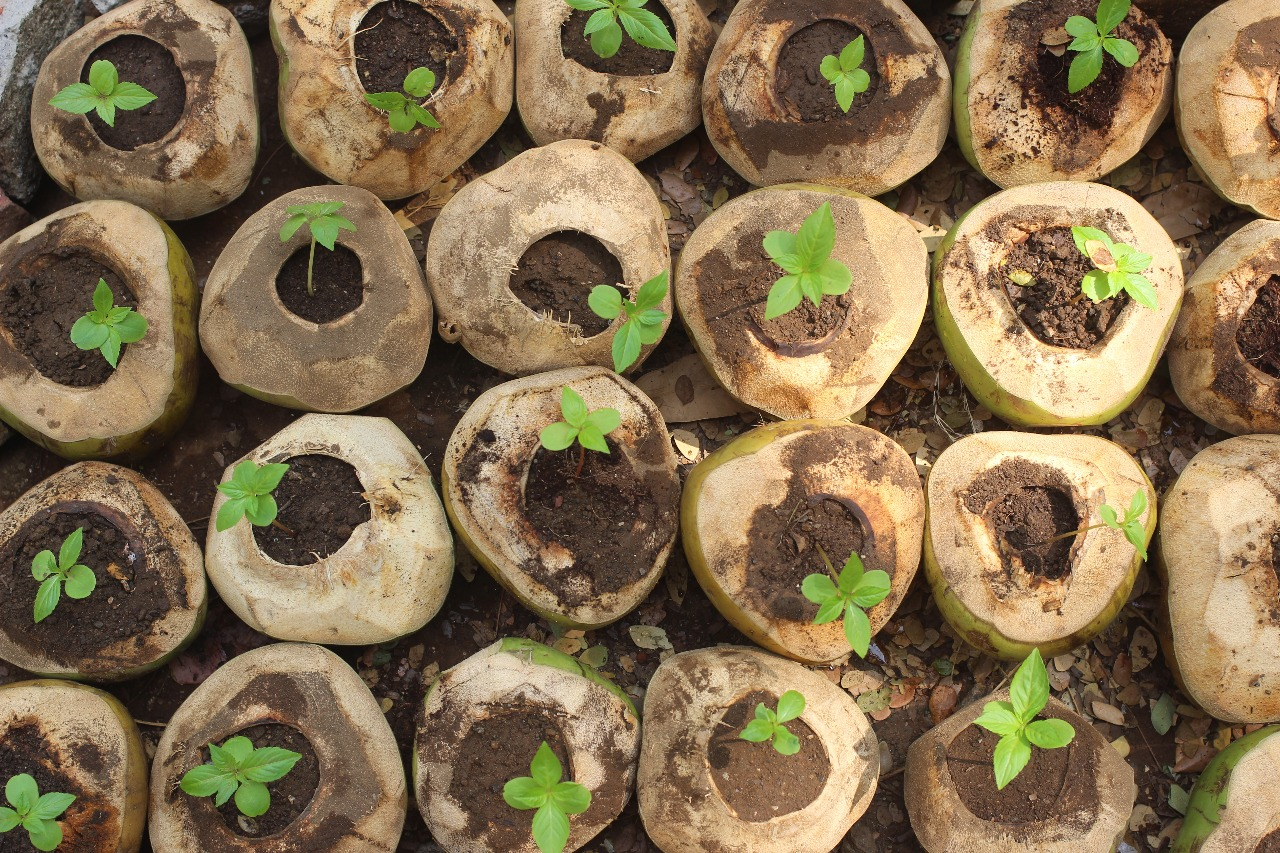
\includegraphics[width = 0.8\textwidth]{g7.JPG}
% \end{subfigure}%
% \begin{subfigure}{.6\textwidth}
% 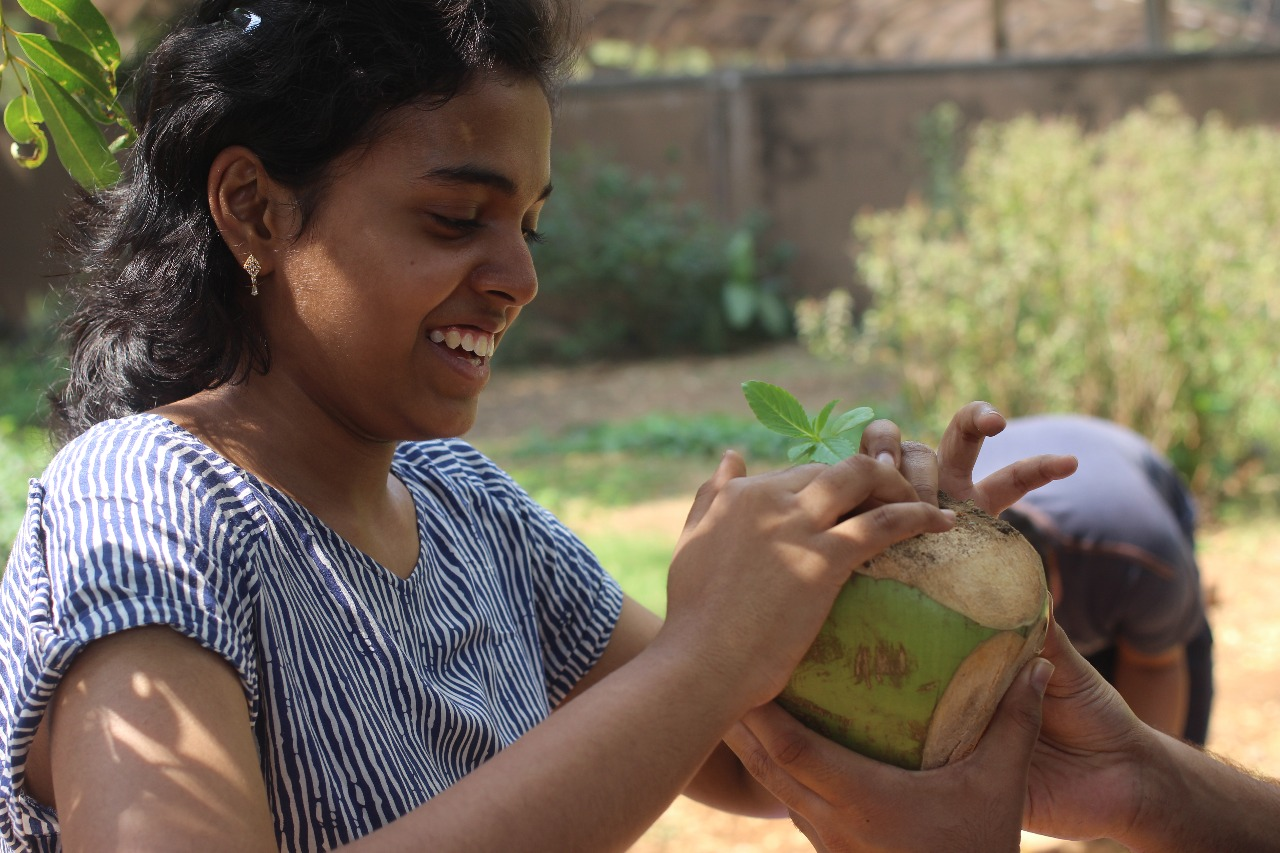
\includegraphics[width = 0.8\textwidth]{g8.JPG}
% \end{subfigure}
% \caption*{Coconut Saplings}
% \end{figure}

% \addcontentsline{toc}{subsection}{ Solar Drip Irrigation:}
% \noindent \textbf{\Large \linebreak \linebreak Solar Drip Irrigation:}\\ \\Aiming to conserve water and demonstrate the idea of smart irrigation, we implemented solar drip irrigation in the nursery.. In this activity, we used plastic bottles that were cut in half and kept inverted at various locations on the bed. After the beds were watered, the evaporated water from the beds got trapped in the bottles, got condensed and went into the beds once again. This helped to keep the bed wet for almost 2-3 days after the day of watering hence reducing the need of daily watering and saving water.\\

% \begin{figure}[H]
% \centering
% 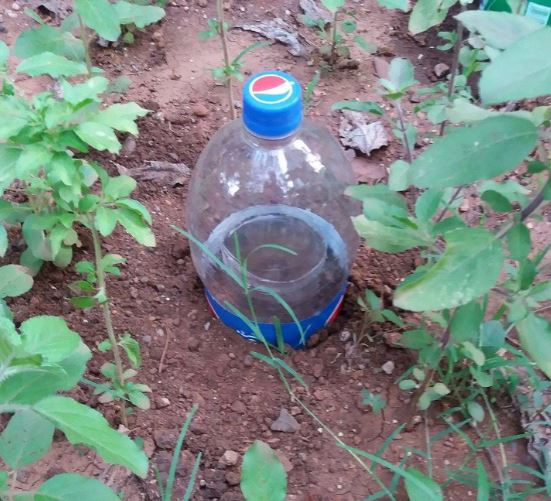
\includegraphics[width = 0.5\textwidth]{g9.jpg}
% \caption*{Solar Drip Irrigation}
% \end{figure}

% \addcontentsline{toc}{subsection}{Nature Walk:}
% \noindent \textbf{\Large Nature Walk:}\\ \\ An insti tour with kids from NGO Vidya was conducted with the main focus to make them realise the various environment related things that we study in textbooks.The walk started from the main gate till the main nursery and later along the lakeside road.There were nearly 50 kids studying in class 6, 7, 8 and 9 who were involved. We plan to make this a major activity from next year and carry it out on a much larger scale.\\

% \begin{figure}[H]
% \centering
% 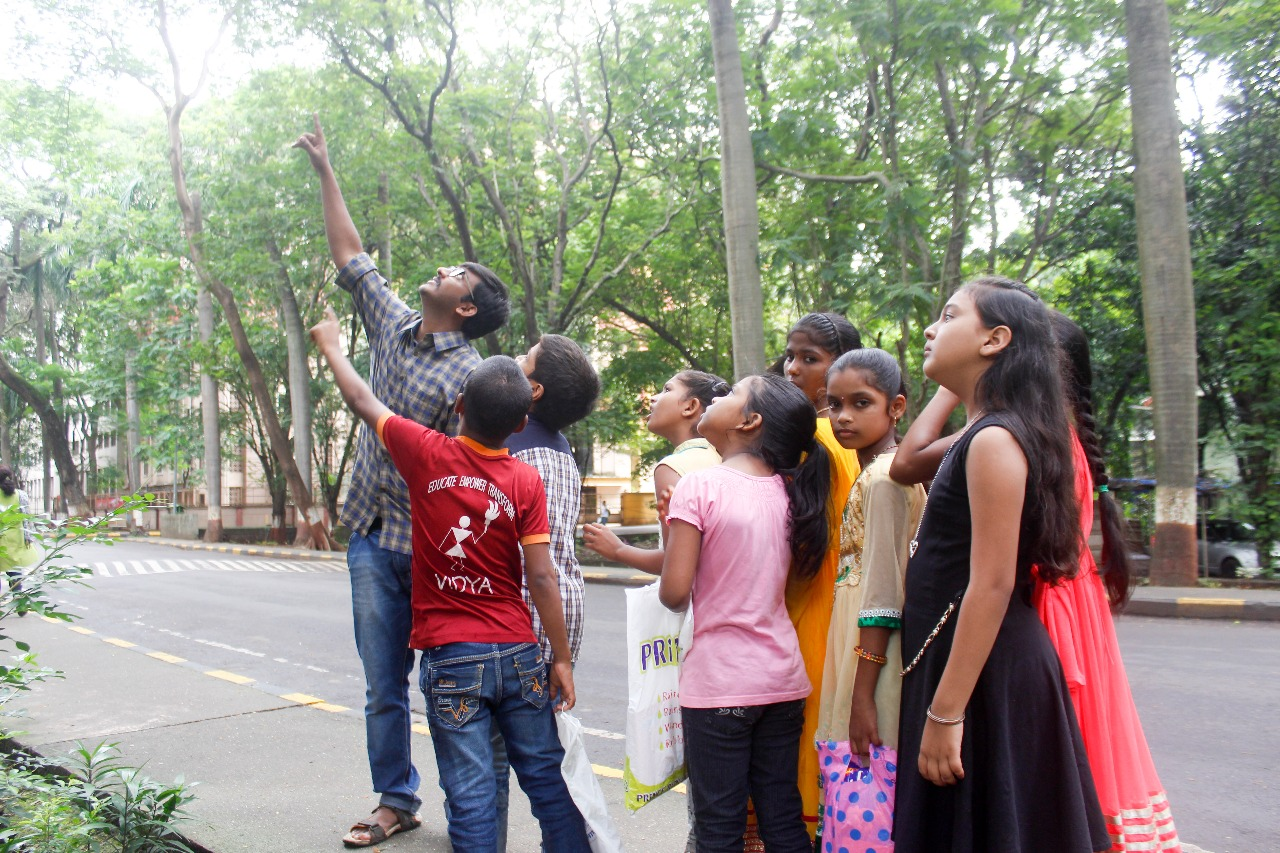
\includegraphics[width = 0.5\textwidth]{g10.jpg}
% \caption*{Nature Walk with kids from NGO Vidya}
% \end{figure}


% \addcontentsline{toc}{subsection}{Nursery for All:}
% \noindent \textbf{\Large Nursery for All:}\\ \\Many residents of the institute are enthusiastic about gardening and maintain pots in their rooms. In case they are not present in the institute for a long time, this initiative gives them an option to safely give their plants a safe shelter during their stay away from the campus in the NSS Nursery. The volunteers at Green Campus water them regularly and take efforts to maintain them. We have officially opened Nursery for visits on Mondays, Wednesdays, and Fridays every week from 5:30-6:00 PM in an academic semester. Apart from this, visitors also have the provision to take saplings to their room, based on the availability in the nursery.\\
% \noindent \textbf{\linebreak Link to Terms and Conditions: } \url {https://tinyurl.com/NurseryForAll} \\

% \addcontentsline{toc}{subsection}{Green Diwali:}
% \noindent \textbf{\Large Green Diwali:}\\ \\ In a first-of-its-kind activity, we made eco-friendly “diyas” using fruit peels.A post was made following this which highlighted the importance of celebrating a pollution free Diwali. Also our volunteers spread the message of celebrating eco-friendly Diwali by writing messages on whiteboard and sharing it on social medias. We plan to involve NGO kids in this activity from next Diwali.\\


% \begin{figure}[H]
% \centering
% 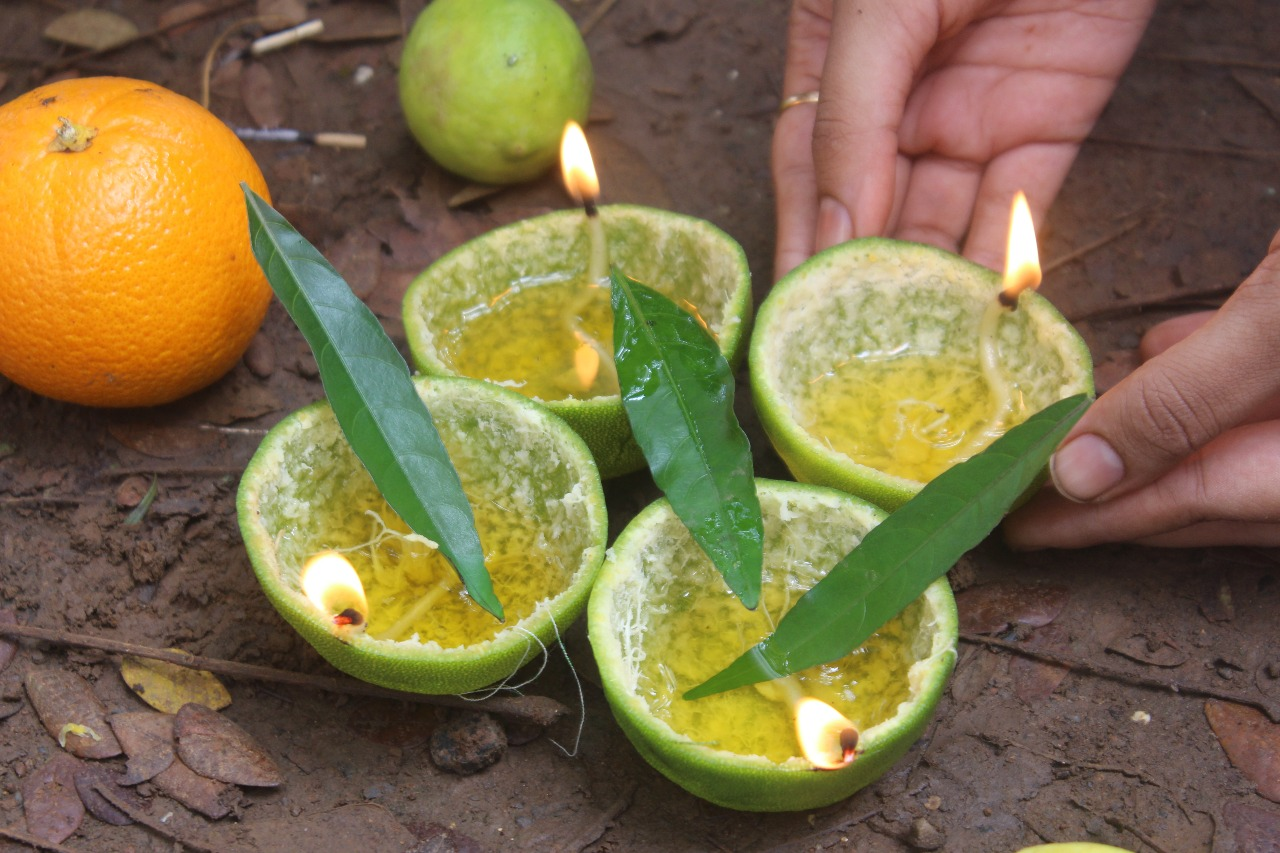
\includegraphics[width = 0.9\textwidth]{g11.JPG}
% \caption*{Green Diwali}
% \end{figure}

% \addcontentsline{toc}{subsection}{Prakriti}
% \noindent \textbf{\Large Prakriti:}\\ \\Prakriti is a discussion and knowledge sharing forum aimed to create awareness about nature. The basic aim is to make people more familiar with gardening and other techniques related to it. People may post any problem they face regarding the same on the forum. Apart from queries and discussion, people can share any interesting information regarding nature. Also, all recent happenings in the NSS nursery are regularly posted.\\

% \noindent \textbf{Ideation:\linebreak}\\ {There are many residents of the campus who are enthusiastic about gardening and want to try out different techniques and explore the field. But very few know where to start! The need was felt for guidance and a platform for all the people who are enthusiastic about exploring gardening. This need gave rise to the idea of Prakriti-A forum for discussion and knowledge sharing.This year a new category named 'Nature and Festivals' was started under which posts on significance of nature in celebrating various festivals were made. }

% \noindent \linebreak Prakriti was started as a google group in August 2016. After starting the blog of NSS, the informative posts on Prakriti are also shared on the blog. Some of the notable informative posts in Prakriti involved Largest trees- Redwoods, Resurrection of the plants-a story of how plants survive the harsh summer, Hemp: A sustainable leap or Narcotic, Medicinal plants in NSS Nursery and communication among honey bees. This year we also started a new category named 'Nature and Festivals' under which we discuss the significance of nature in celebrating various festivals. Under this, we have covered 'Holi', 'Makar Sankranti','Diwali' etc. Some people also came up with their queries like cutting of the trees, initiation of a nursery in hostel 13. Till date we have approximately 300 members. We hope to reach out to people who are more proactive so that they can help solve the queries of group members whenever required.


% \noindent \textbf{\linebreak Link: } \url{prakriti_nssiitb@googlegroups.com} \\
% \noindent \textbf{Link: } \url{https://groups.google.com/group/prakriti_nssiitb}\\
% \noindent \textbf{Link: } \url{https://nssiitbblog.wordpress.com/category/green-campus/prakriti/
% } \\

% \addcontentsline{toc}{subsection}{Summer Volunteering in the Nursery:}
% \noindent \textbf{\Large \linebreak Summer Volunteering in the Nursery:}\\ \\ Unavailability of first year volunteers during summers lead to the idea of involvement of non NSS people as volunteers. Main idea was to extend the reach of NSS to people who are enthusiastic about gardening or want to explore it. 90+ students showed interest in the summer volunteering program and 70+ among them were postgraduate or Ph.D students.
% These volunteers helped in watering and regular maintenance of the nursery during the harsh summer days. Plantation on the occasion of World Environment Day was carried out by these volunteers. \\ \\

% \addcontentsline{toc}{subsection}{Blog writing:}
% \noindent \textbf{\Large Blog writing:}\\ \\ In this activity, each volunteer had to find out about an interesting topic, that was also found by themselves, related to nature. Then in a group of 12-15 they presented the topic and all of them  had a discussion on it. The team members made blog posts considering whatever points were discussed in this meet. These blog posts were released online via WordPress. \\ \\

% \pagebreak
% \chapter*{Vikas}
% \markboth{Vikas}{Vikas}
% \addcontentsline{toc}{chapter}{Vikas}
% \addcontentsline{toc}{section}{About the Department}
% \section*{\LARGE About the Department:}Vikas means progress and development. We focus on identifying existing problems and come up with 'What can I do' level solutions so that everyone can implement them and contribute their bit to the society. This year around we decided to focus on sustainable development. We carried out activities that promote awareness about sustainability and encourage people to adopt a sustainable lifestyle. Through dedicated efforts, we tried to bring some small changes in and around the campus.


% \addcontentsline{toc}{section}{Major Activities}
% \section*{ \LARGE Major Activities}
% \addcontentsline{toc}{subsection}{Eco-friendly Ganesha Idols}
% \noindent \textbf{\Large Eco-friendly Ganesha Idols:}\\ \\
% Ganesh Clay idol making is one awareness and change activity that we immediately need to practice. Many NSS and non-NSS volunteers participated in the clay-idol making workshop organized by the staff club of IIT Bombay. Apart from this, 6 hostels enthusiastically celebrated the festival with the eco friendly idols made in he staff club leading to minimum pollution. Some people also decided to travel an extra mile on the eco friendly road and chose to put seeds inside the idols which where then immersed in a pot rather than water bodies and grown into beautiful plants.
% The idols made by NSS volunteers were distributed among the PHO workers assisting them to celebrate festival in an economical as well as eco-friendly way.\\

% \begin{figure}[H]
% \centering
% 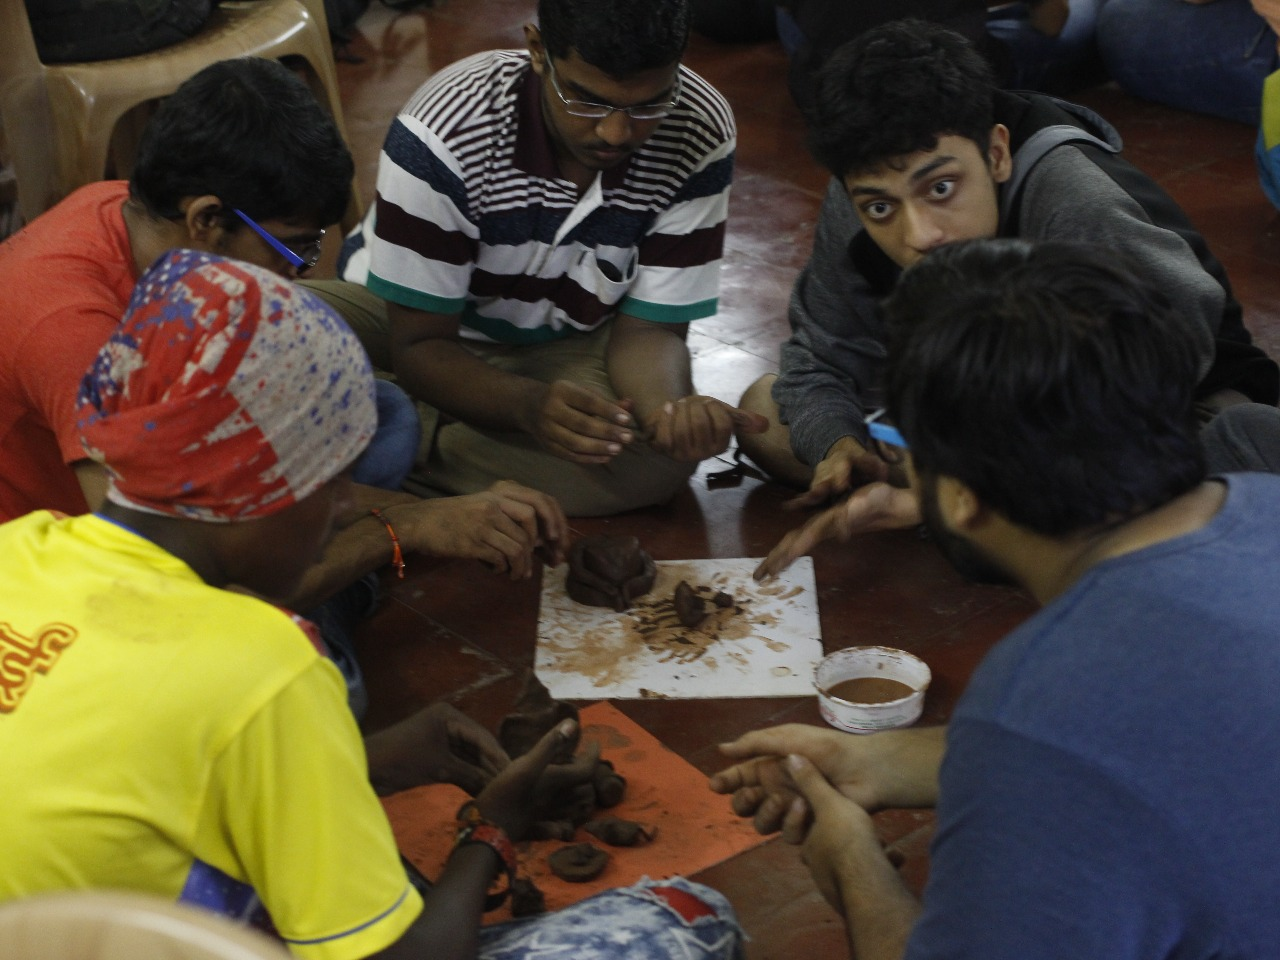
\includegraphics[width = 0.9\textwidth]{v2.JPG}
% \caption*{Volunteers making idols from clay}
% \end{figure}

% \addcontentsline{toc}{subsection}{Animal Vaccination Drive}
% \noindent \textbf{\Large \linebreak Animal Vaccination Drive:}\\ \\The Animal Rescue Group of IIT Bombay, consisting of professors, students and campus residents, led by Prof. Madhu Belur and Prof. Prita Pant, organized the annual animal vaccination drive in the institute. The vaccinations were carried out by members of The Welfare of Stray Dogs organization. NSS IITB volunteers helped in the vaccination process and also maintained the database of the vaccinated dogs. Around 85 dogs were vaccinated. We were delighted to see that many people came forward to help when the vaccinations were being conducted in their hostels, or near their residential areas.

% \begin{figure}[H]
% \centering
% 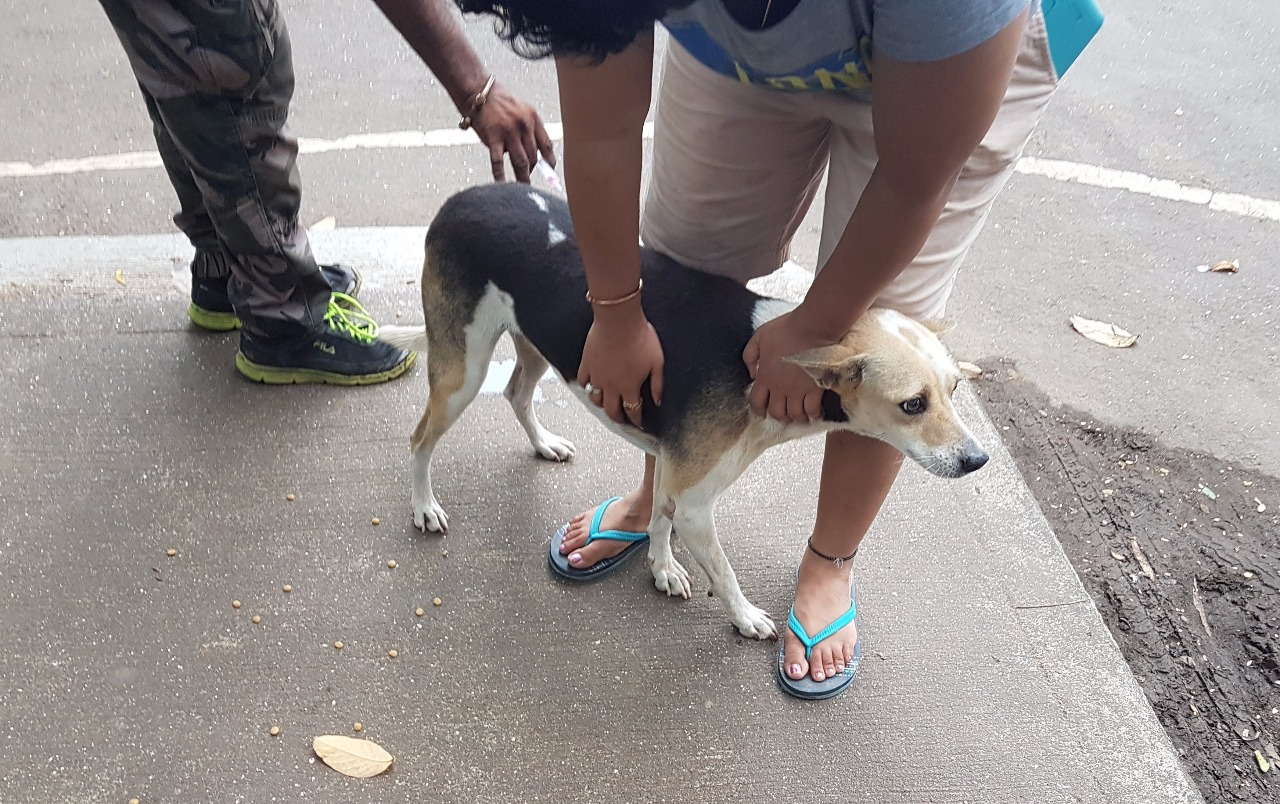
\includegraphics[width = 1.0\textwidth]{v1.jpg}
% \end{figure}

% \addcontentsline{toc}{subsection}{Reducing Food Wastage:}
% \noindent \textbf{\Large \linebreak Reducing Food Wastage::}\\ \\
% The volunteers made posters on reducing food wastage which were put on in many hostel messes. Apart from this, we also conducted a survey spanning all the messes to find out the amount of wastage of raw and cooked food, the leftovers and the variation in the same with the menu that day.
%  \\

% \addcontentsline{toc}{subsection}{Best out of Waste}
% \noindent \textbf{\Large \linebreak Best out of Waste:}\\ \\
% A large number of flex banners are used in the institute throughout the year. We innovatively came up with some ideas of reusing these waste flexes. These were collected by our volunteers and were made into sapling covers and flex carry bags. Flex bags were distributed in the campus shops whereas the sapling covers rest in peace in the NSS nursery caressing tender saplings. Apart from these, we also made stationary pouches to be used by kids.\\ \\ \\ \\ \\ \\

% \begin{figure}[H]
% \centering
% \begin{subfigure}{.5\textwidth}
%  \centering
%  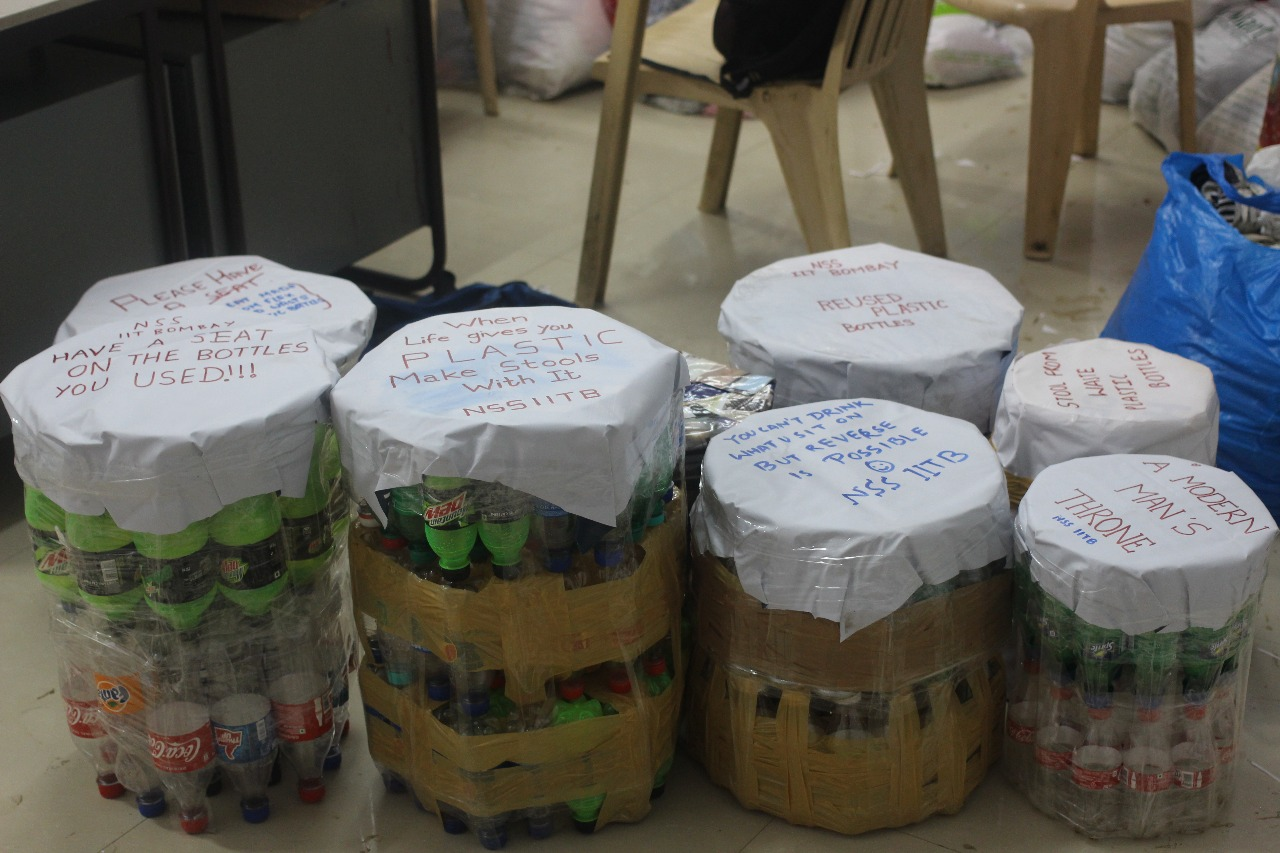
\includegraphics[width = 0.9\textwidth]{v5.JPG}
% \end{subfigure}%
% \begin{subfigure}{.5\textwidth}
% 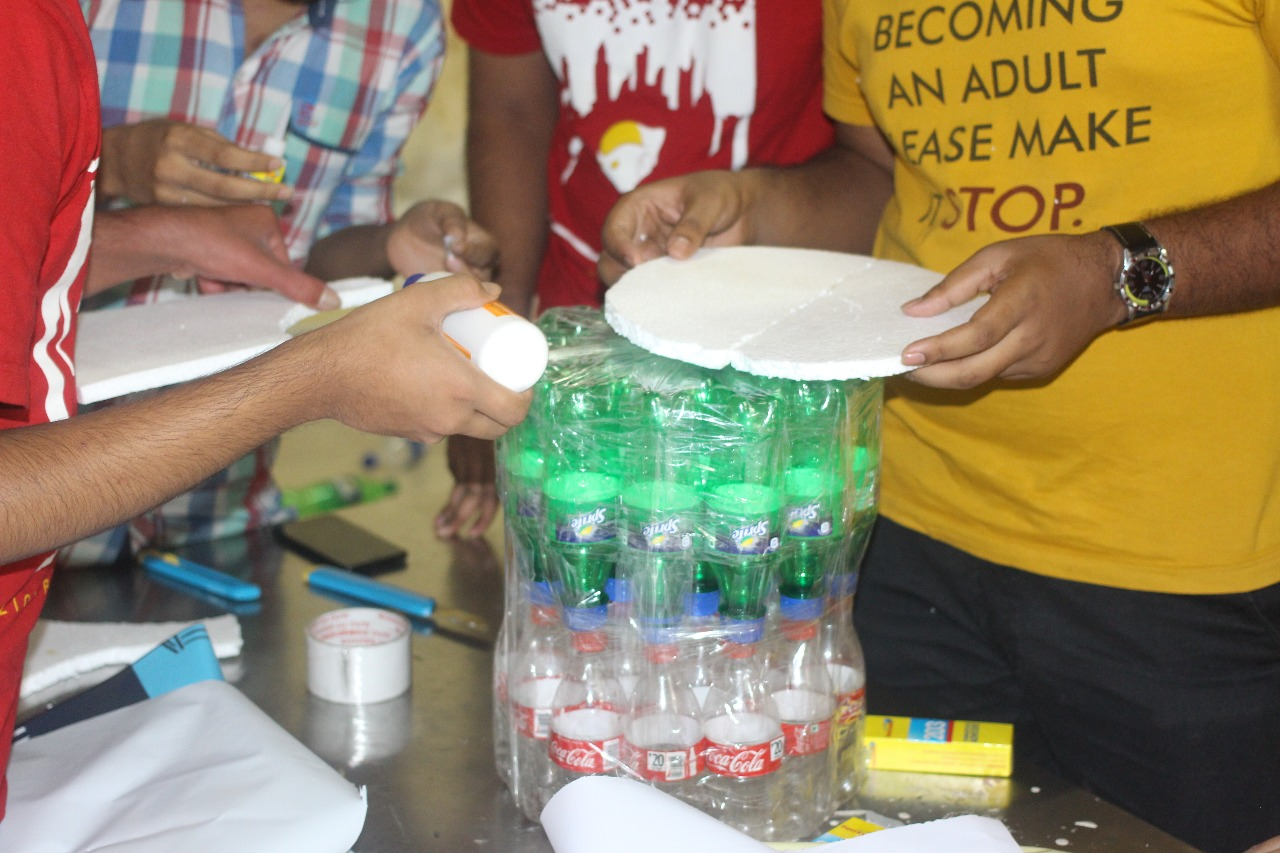
\includegraphics[width = 0.9\textwidth]{v6.JPG}
% \end{subfigure}
% \caption*{Reusing of Plastic Bottles}
% \end{figure}

% We believe that many want to recycle plastic but don’t know how to proceed. In order to set an example of  recycling plastic, the volunteers collected used plastic bottles and assembled them together to make stools. The stools were covered with multiple layers of used flexes. The stools were kept at locations where there were no place to sit. In our opinion, these stools, besides being an easy and inexpensive make, will also serve the purpose of spreading the idea of sustainability.

% \addcontentsline{toc}{subsection}{Tarang - The Sustainability Club}
% \noindent \textbf{\Large \linebreak \linebreak Tarang - The Sustainability Club
% }\\ \\
% Under Tarang - the sustainability initiative, a new chapter has been started by NSS IIT- Bombay in the form of BMC school visits. The vision behind this initiative to promote Sustainability among young minds and to inculcate the very idea at the grassroot level.We conduct sessions in schools for students of class 7th to 10th which focus on instilling the importance of saving resources, reusing, recycling and incorporating sustainable practices in day-to-day lives.
% As of now we have visited 8 schools and presented two different modules to help the cause.

% \begin{figure}[H]
% \centering
% 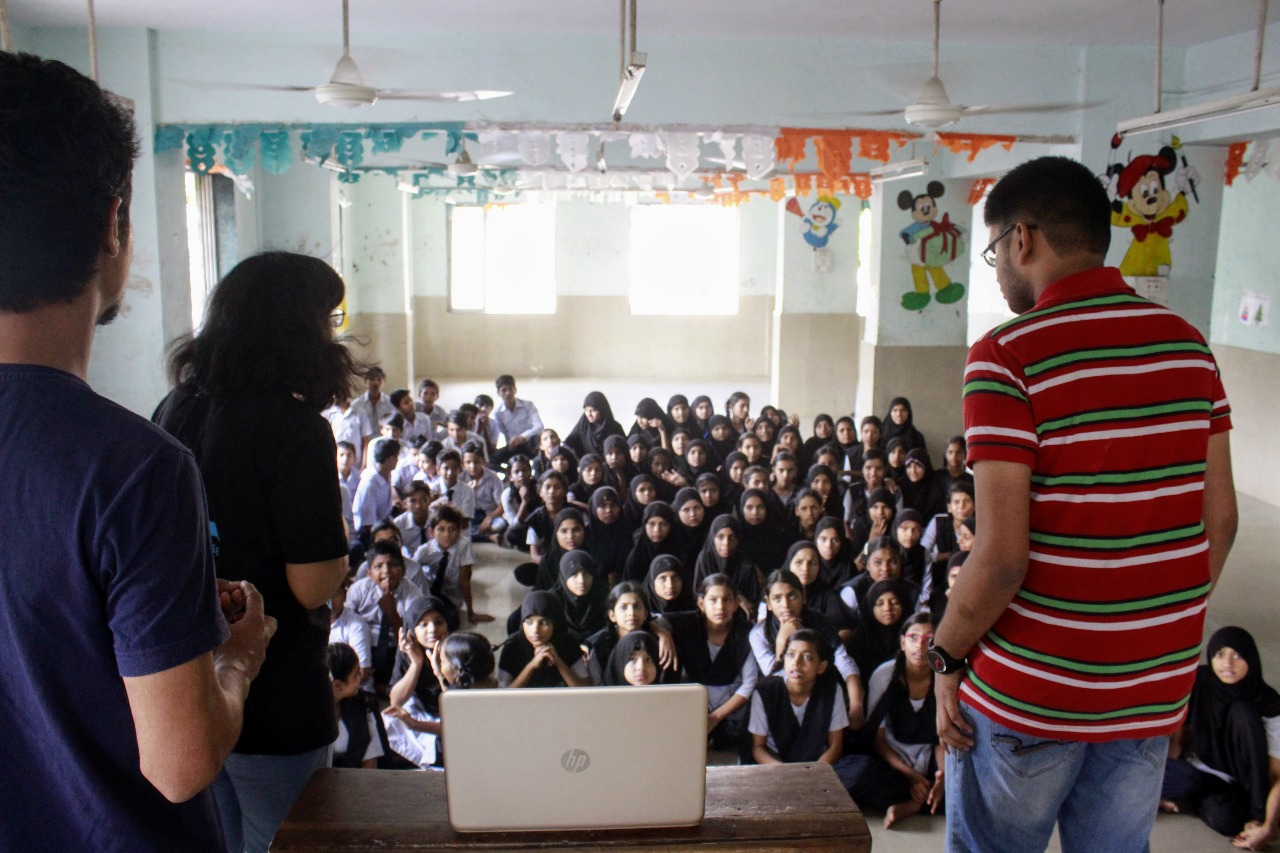
\includegraphics[width = 0.65 \textwidth]{v3.jpg}
% \caption*{Session in a BMC School}
% \end{figure}

% \addcontentsline{toc}{subsection}{Carbon and Water Footprint Audit:}
% \noindent \textbf{\Large \linebreak Carbon and Water footprint Audit:}\\ \\
% The idea behind this activity was to bring out two important quantitative measures of the extent to which our day-to-day activities affect the environment. It started with a talk given by Prof. Yogendra Shastri, Chemical Engineering department who guided the volunteers about the approach to take for the calculation of the two footprints.\\ \\
% Volunteers made charts which were put up in the messes of hostel 15 and 16 to assist freshmen in calculating their own footprints with ease. Apart from this, the volunteers also calculated carbon and water footprints making comparison among different hostels, department buildings and eateries in the campus.
% \\ \\

% \addcontentsline{toc}{subsection}{Phulenagar Slum Visit:}
% \noindent \textbf{\Large \linebreak Phulenagar Slum Visit:}\\ \\
% We visited the phule nagar slum to enquire closely into the world of people who reside there. We figured out significant information related to their family strength and composition, the societal problems they might be facing, schooling of kids, water and electricity pains prevalent in homes, method of waste disposal and the common diseases prevalent there. We found that the residents there were enthusiastic to interact with us and willingly gave us all the information we asked for. A conclusion drawn from the visit was that there was no proper waste disposal there which had become a root cause of many diseases.
% \\ \\
% \begin{figure}[H]
% \centering
% 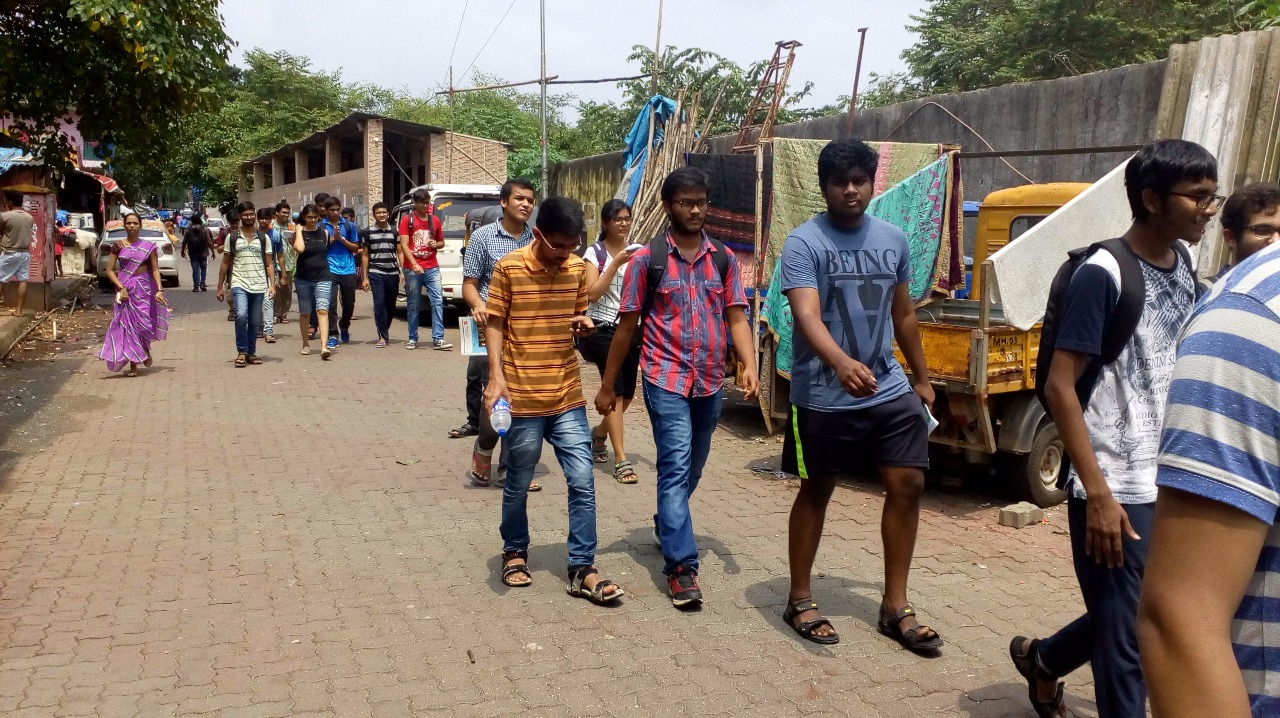
\includegraphics[width = 0.9 \textwidth]{v4.jpg}
% \caption*{Phulenagar Slum Visit}
% \end{figure}

% \chapter*{Events}
% \markboth{Events}{Events}
% \addcontentsline{toc}{chapter}{Events}

% \addcontentsline{toc}{section}{About the Department}
% \section*{\huge About the Department:} Events is the department of NSS, IIT Bombay that believes in the ‘Upliftment of the poor section of society through change in lifestyle.’ We at Events strive to ensure that various activities that are performed to achieve the above-mentioned initiatives, are undertaken in an extensive and optimized manner. From the students at the Aman Day center in the institute to the tribal areas in the outskirts of the city, the department has had many beneficiaries and with new initiatives kicking in, the number is bound to increase.

% \addcontentsline{toc}{section}{Major Activites:}
% \section*{\huge Major Activities:}

% \addcontentsline{toc}{subsection}{Graduating Students' Collection Drive}
% \noindent \textbf {\Large Graduating Students' Collection Drive:}\\ \\“Before this, we used to sleep on the ground...but now, things will change”’- A Construction Worker in Ambernath
% \linebreak
% Every year, the institute witnesses the passing out of a large no. of students, both at the under-graduation and the post-graduation level. The students that pass out, often leave their bulky belongings, like mattresses, pillows, buckets etc. here, as they are not needed anymore. The Graduation Collection Drive(GCD) was started with the thought that these items, if collected and donated, could be effectively used to benefit a large section of the society i.e. a complete village or a colony. The activity is generally done by the Activity Associates of the departments, under the supervision of the Department Heads. Volunteers are included in the donation activities Every year, the initiative is held in the months of May and June, as it is the time when the academic year ends and the students leave. This year, the donation activities were held in the slum areas of Ambernath.

% \begin{figure}[H]
% \centering
% \begin{subfigure}{.5\textwidth}
%  \centering
%  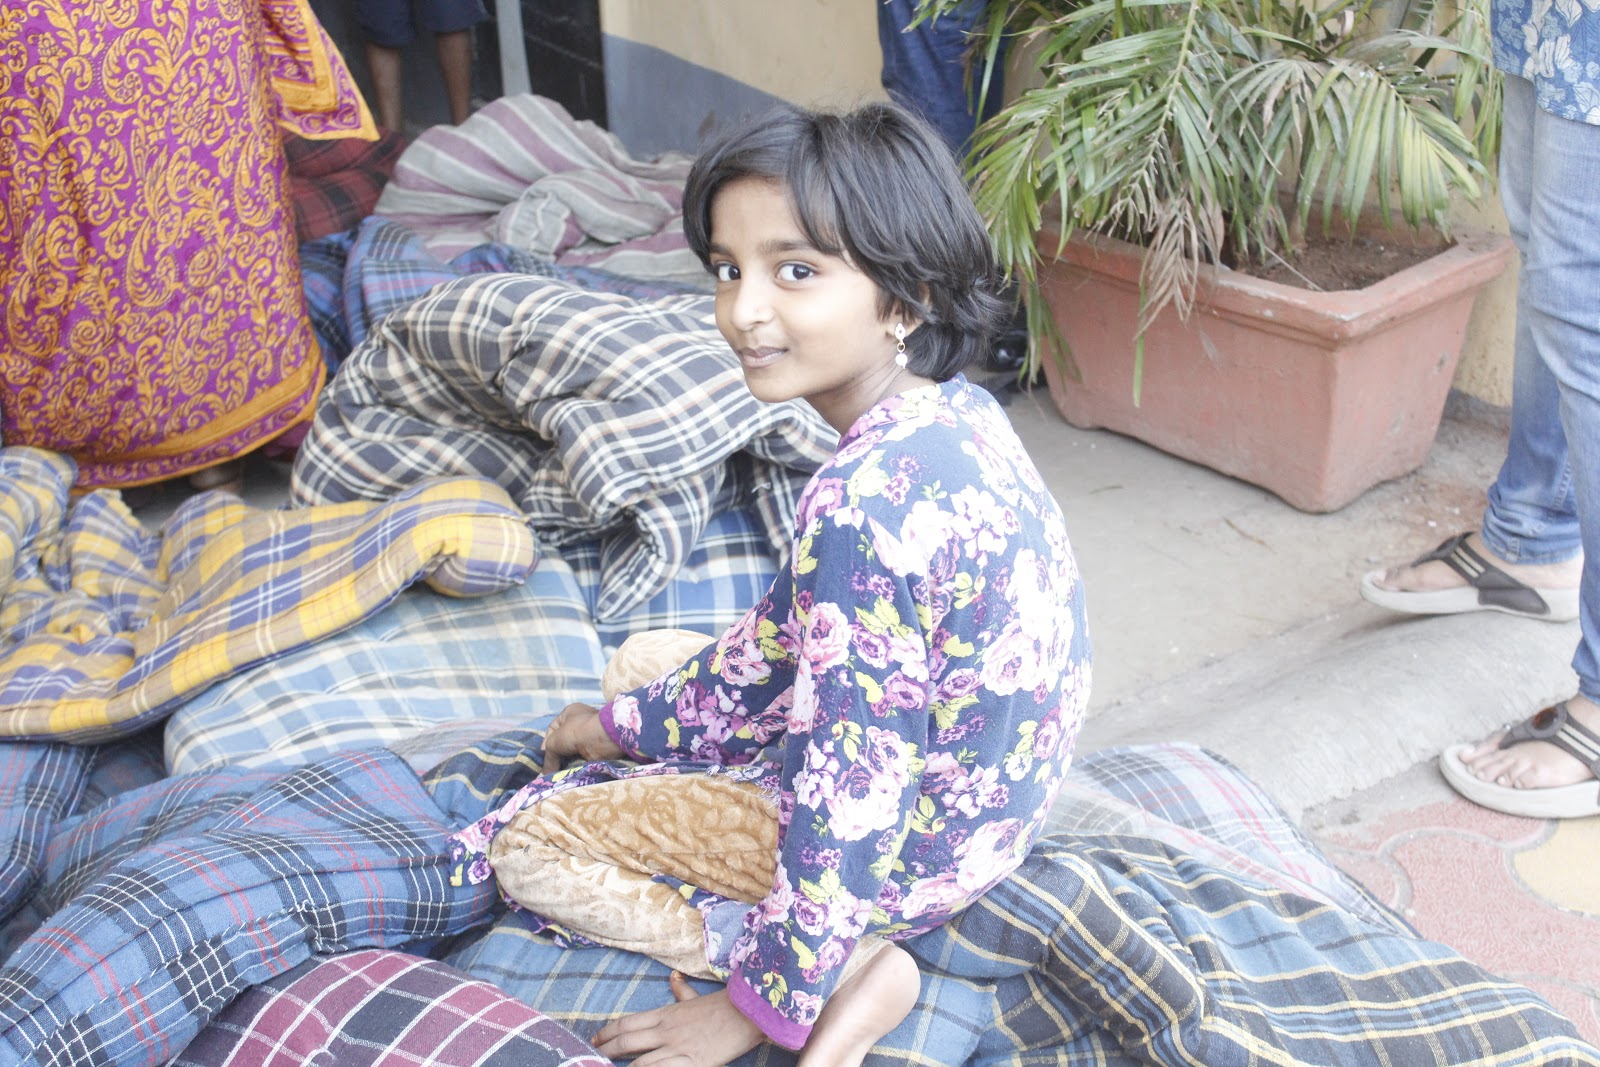
\includegraphics[width = 0.9\textwidth]{e1.jpg}
% \end{subfigure}%
% \begin{subfigure}{.5\textwidth}
% 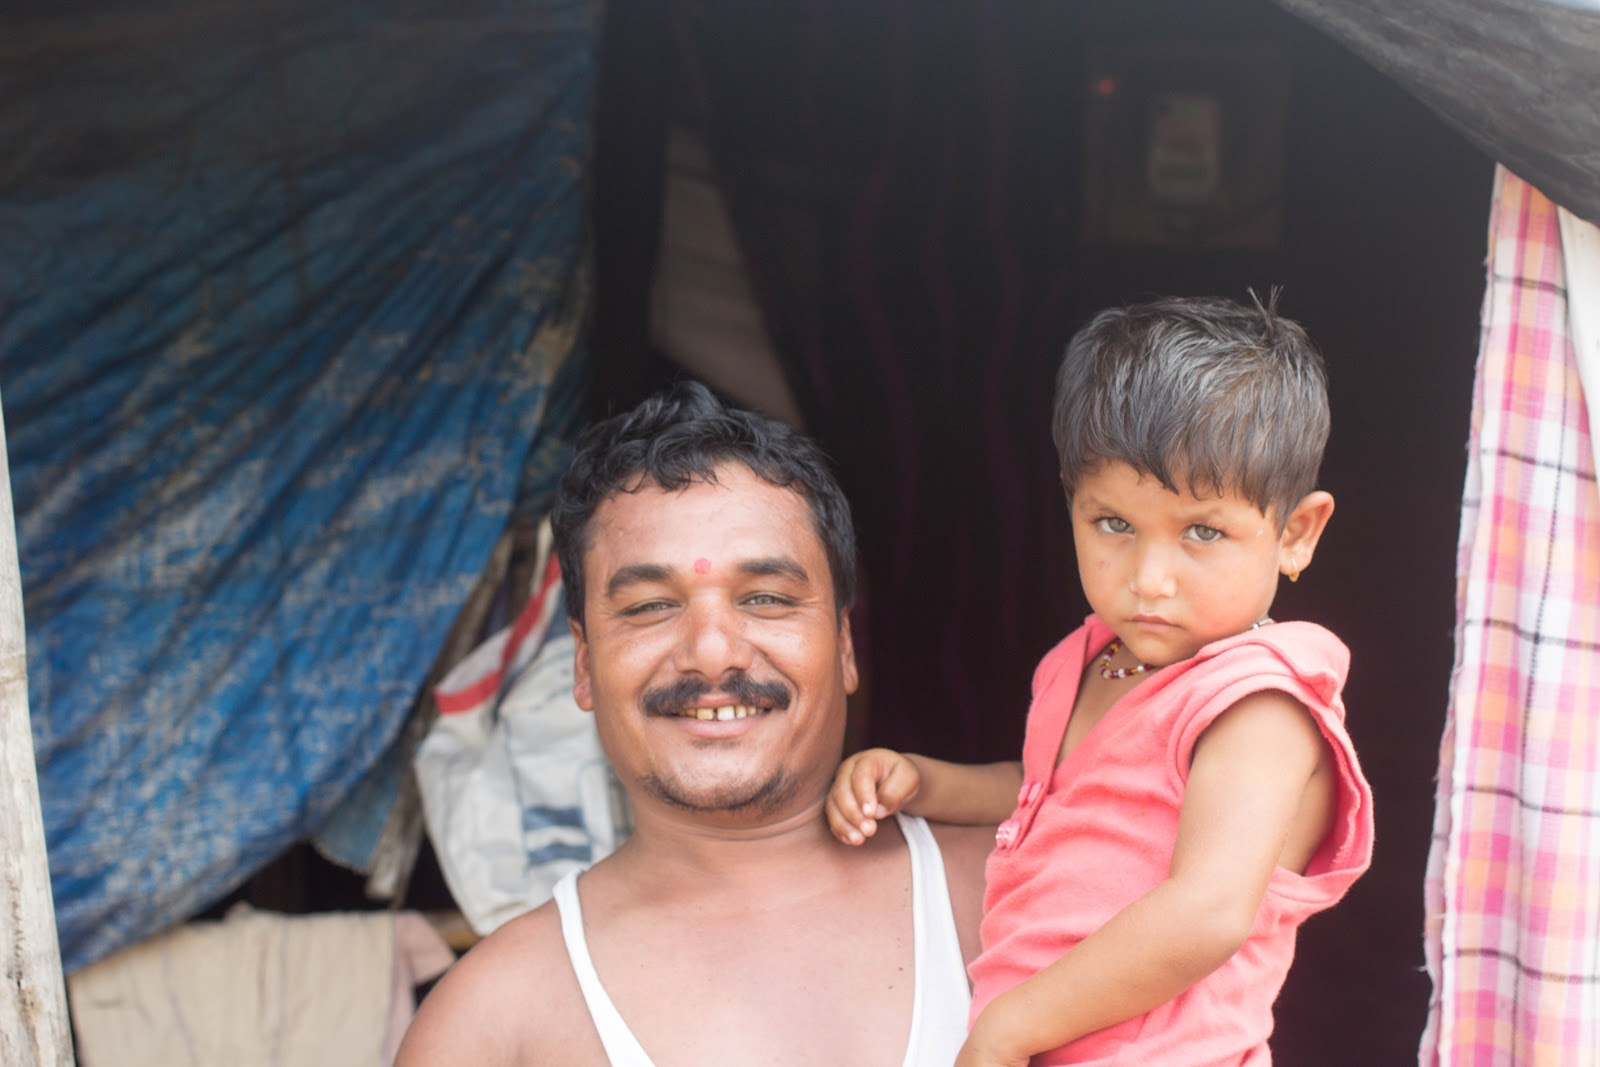
\includegraphics[width = 0.9\textwidth]{e2.jpg}
% \end{subfigure}
% \end{figure}

% \begin{figure}[H]
% \centering
% \begin{subfigure}{.5\textwidth}
%  \centering
%  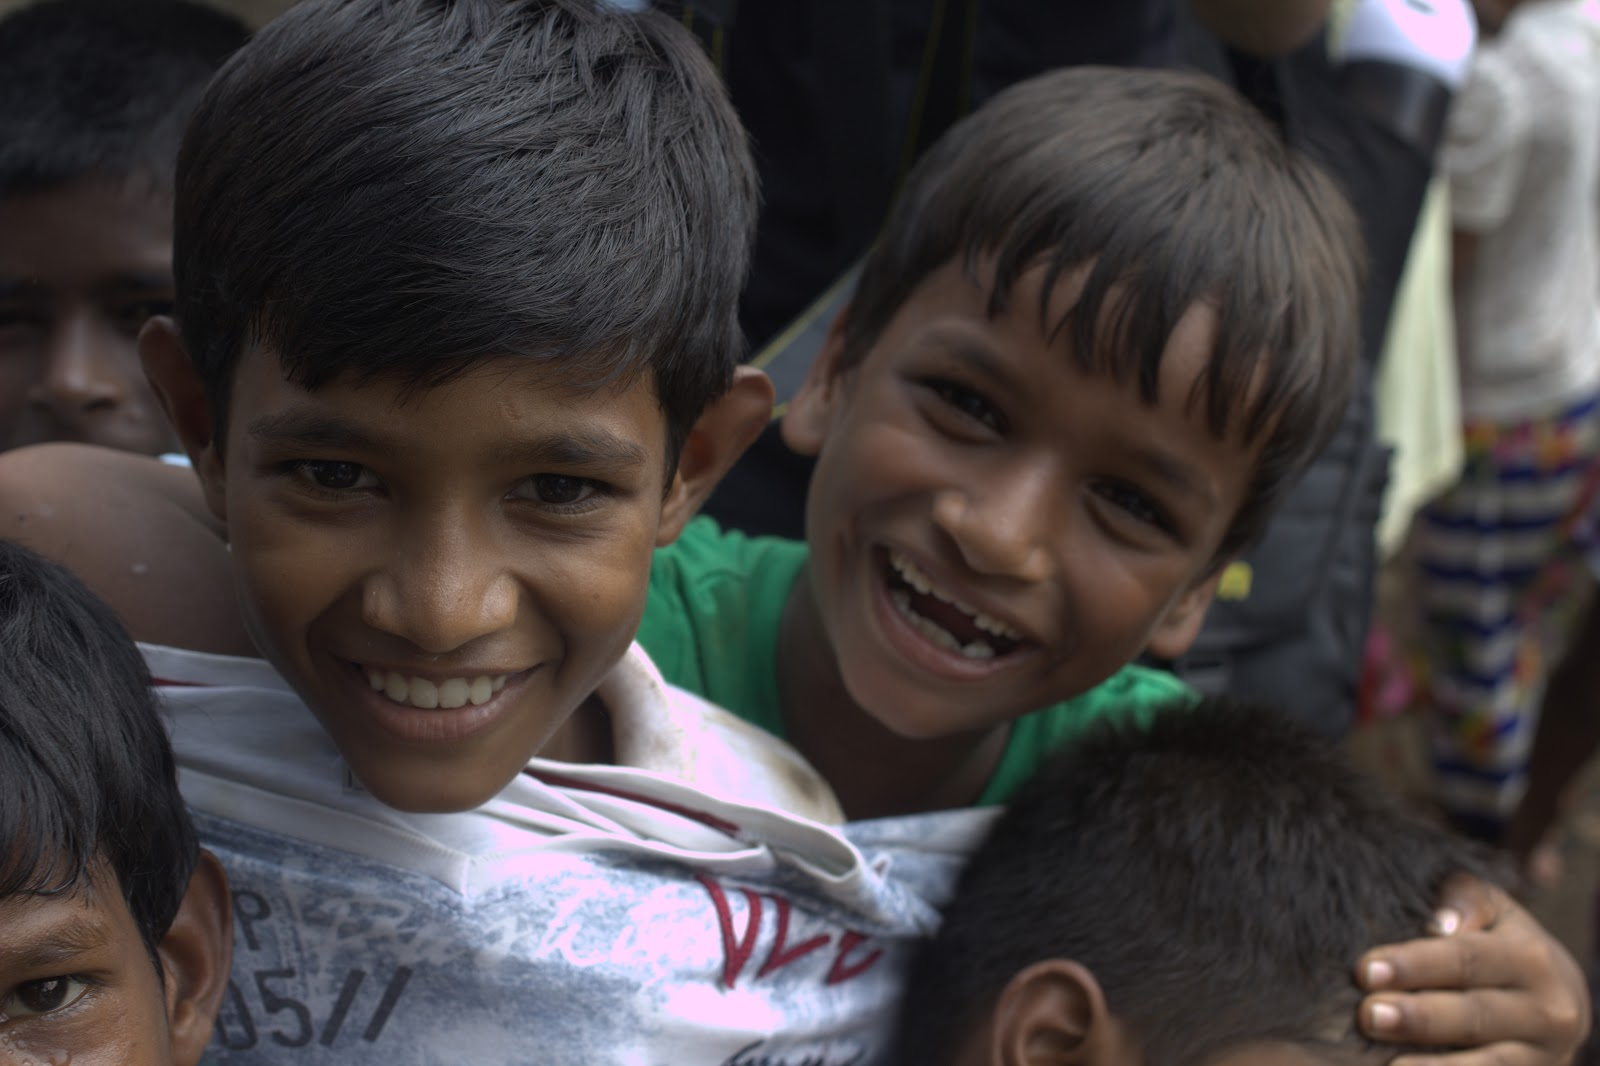
\includegraphics[width = 0.9\textwidth]{e3.jpg}
% \end{subfigure}%
% \begin{subfigure}{.5\textwidth}
% 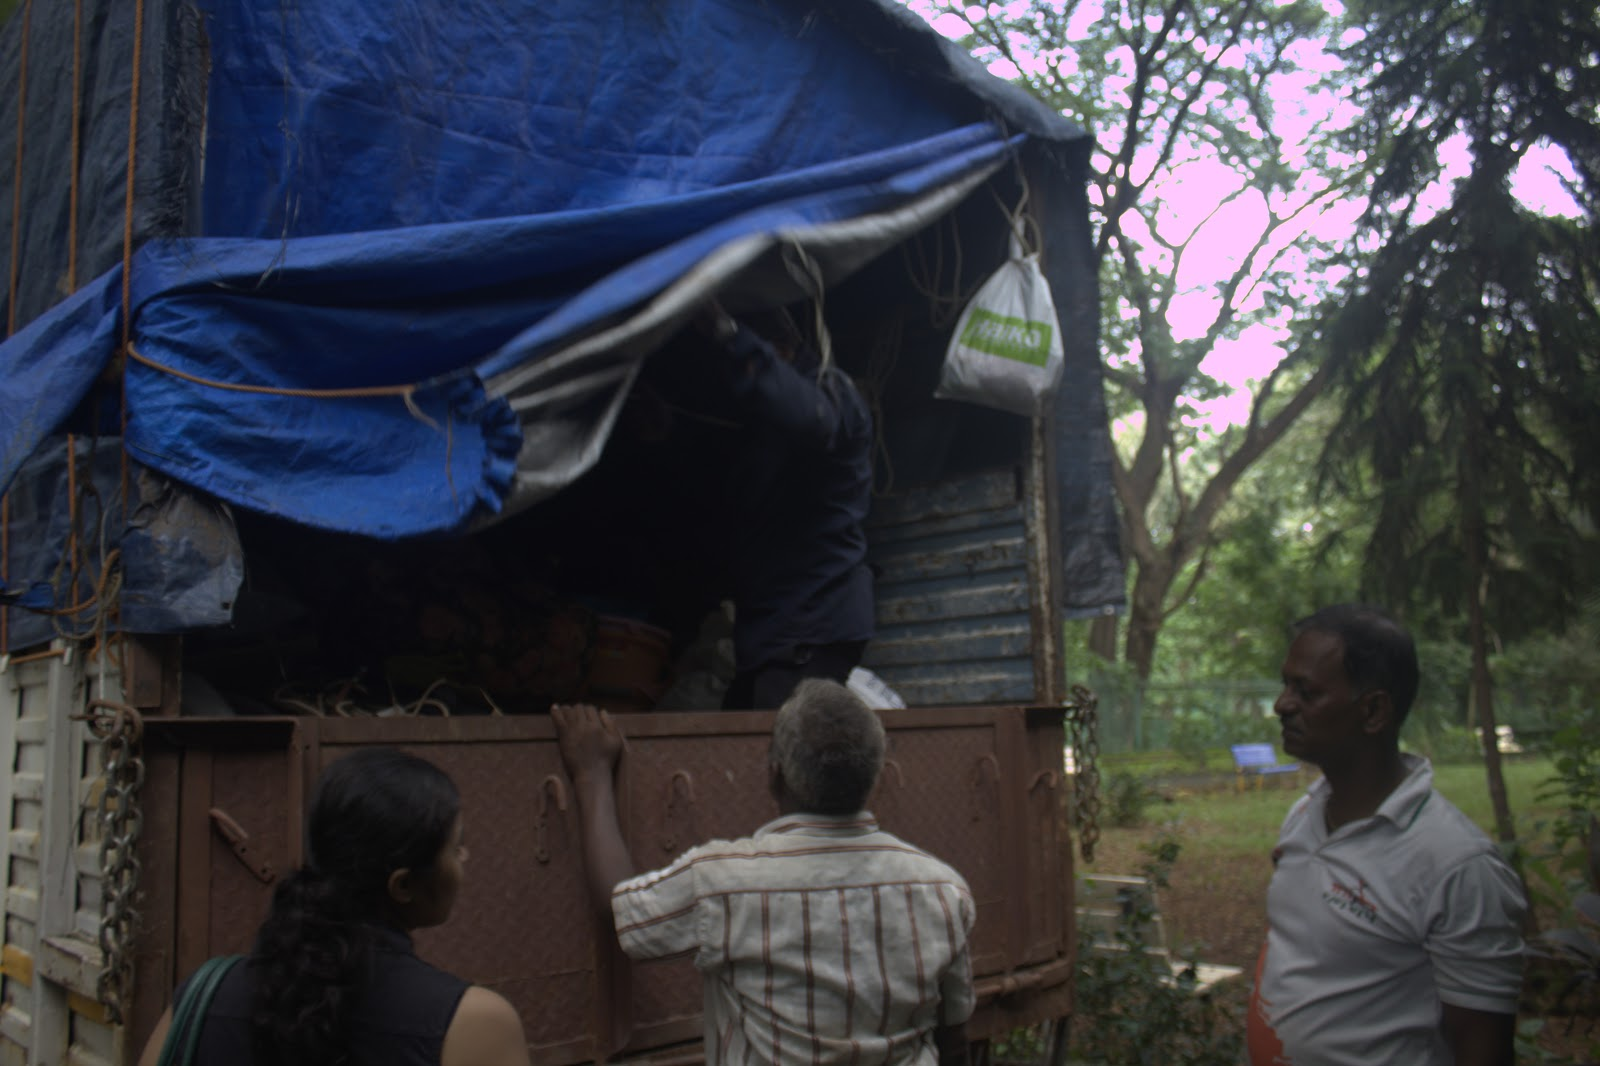
\includegraphics[width = 0.9\textwidth]{e4.jpg}
% \end{subfigure}
% \end{figure}

% \addcontentsline{toc}{subsection}{Cloth Collection Drive}
% \noindent \textbf {\Large \linebreak Cloth Collection Drive:}\\ \\As the name suggests, the initiative acts as a link between the donation-interested people in the institute to the beneficiaries by donation of clothes from the former to latter. As the flagship activity of the Events Department, the Cloth Collectin Drive(CCD) is held over the course of the complete academic year. It is further broken down to 2 phases- Phase 1, held in October involves collection from the student hostels, which includes making of interactive donation boxes by the volunteers, putting them up in visible, common areas in each hostel followed by regular collection of the donated items. Phase 2, held in March, is conducted in the professor residences, the volunteers are divided into specific groups and allotted specific areas, where at first publicity posters are put up, followed by 4-5 visits in the areas to collect clothes from the interested people. In both the phases, segregation and sorting of clothes are done by the volunteers itself. The activity is most enjoyed by volunteers as they themselves are responsible for all the collection, the sorting and the donation activities done in the initiative. This year, the initiative, especially Phase 1 witnessed a huge growth in terms of the volume of clothes donated. The phase 1 donations were again carried out in the slum areas of Ambernath, with the help of The Front Labour Union, over the course of two visits. The head of the front labour union said the following about our initiative:
% \linebreak
% \linebreak
% “You all are doing a great work. I have never seen college students affecting the lives of such a large group of people in this type of effective and efficient way”
% \\ \\
% \begin{figure}[H]
% \centering
% \begin{subfigure}{.5\textwidth}
%  \centering
%  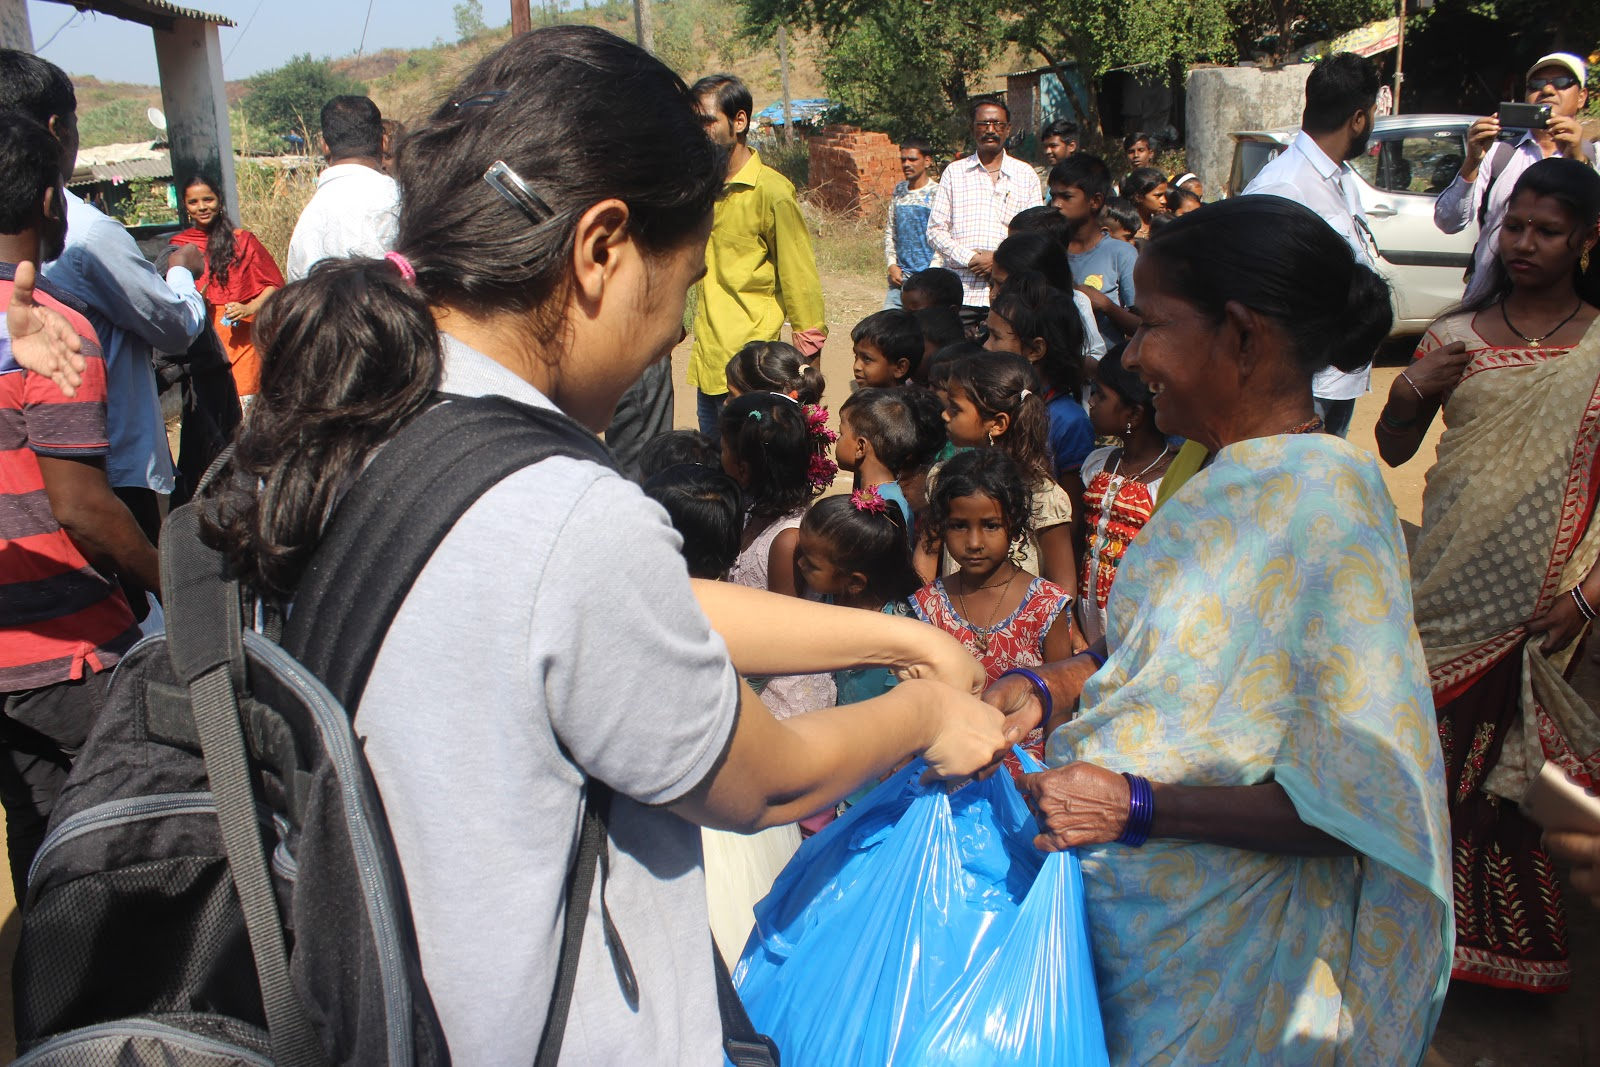
\includegraphics[width = 0.9\textwidth]{e5.jpg}
% \end{subfigure}%
% \begin{subfigure}{.5\textwidth}
% 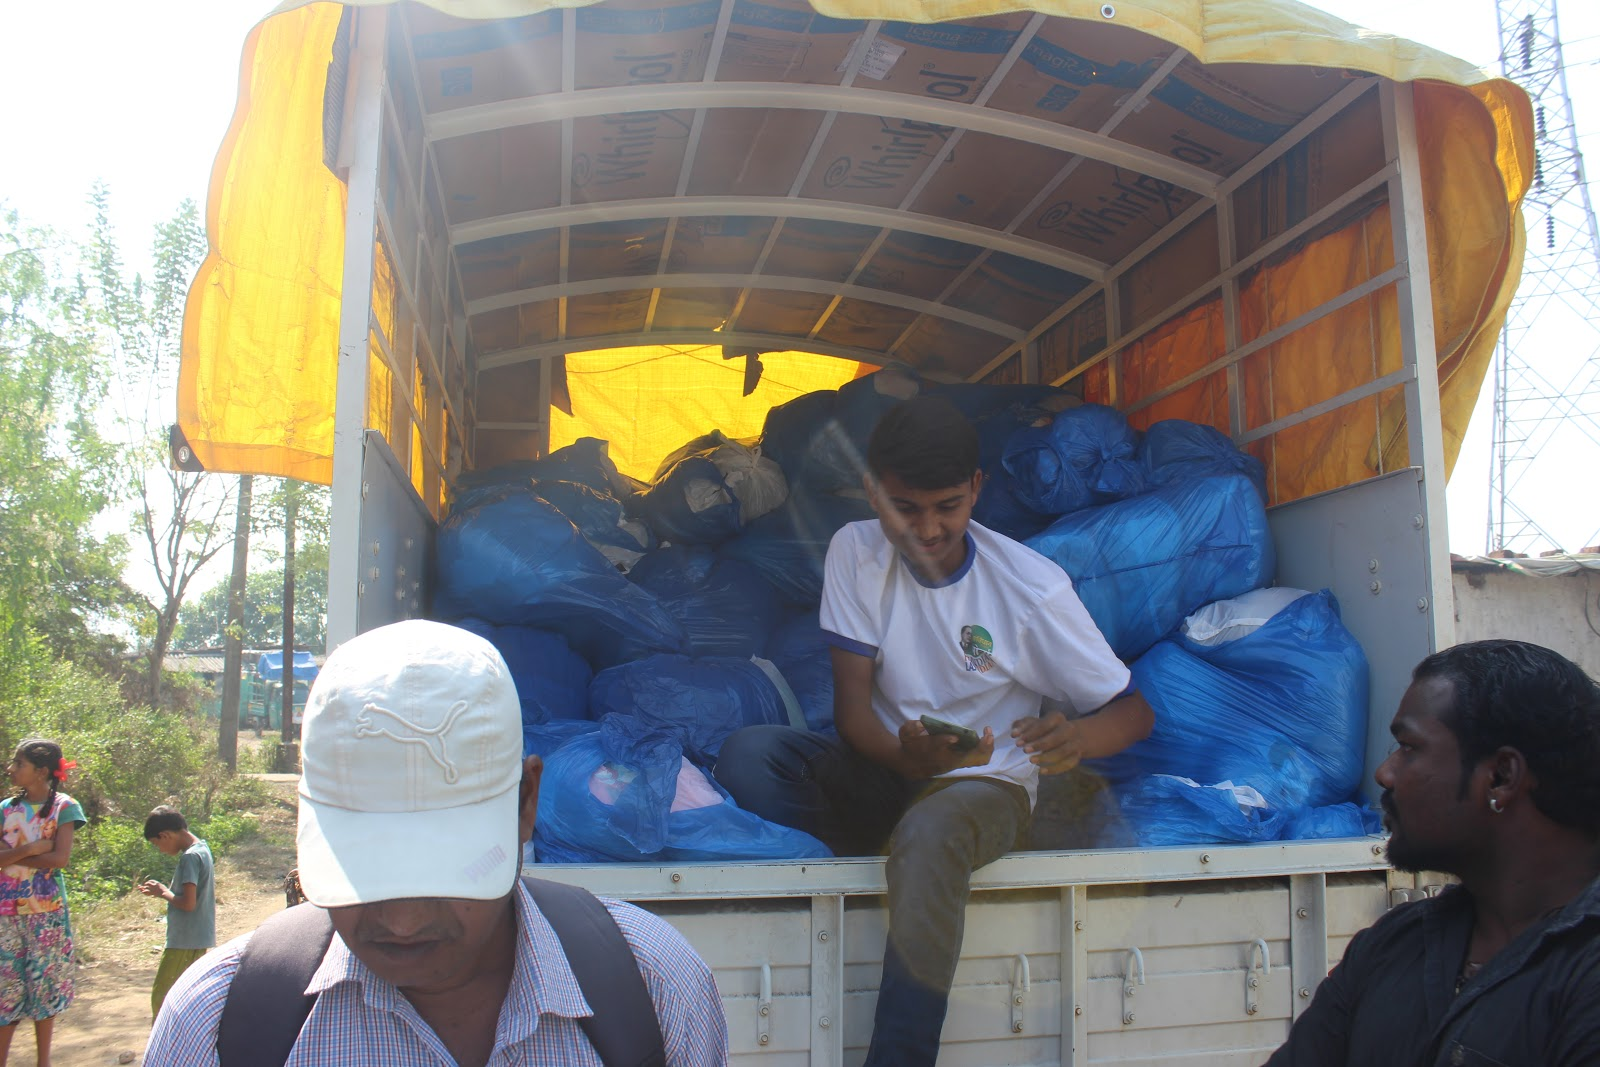
\includegraphics[width = 0.9\textwidth]{e7.jpg}
% \end{subfigure}
% \end{figure}

% \begin{figure}[H]
% \centering
% \begin{subfigure}{.5\textwidth}
%  \centering
%  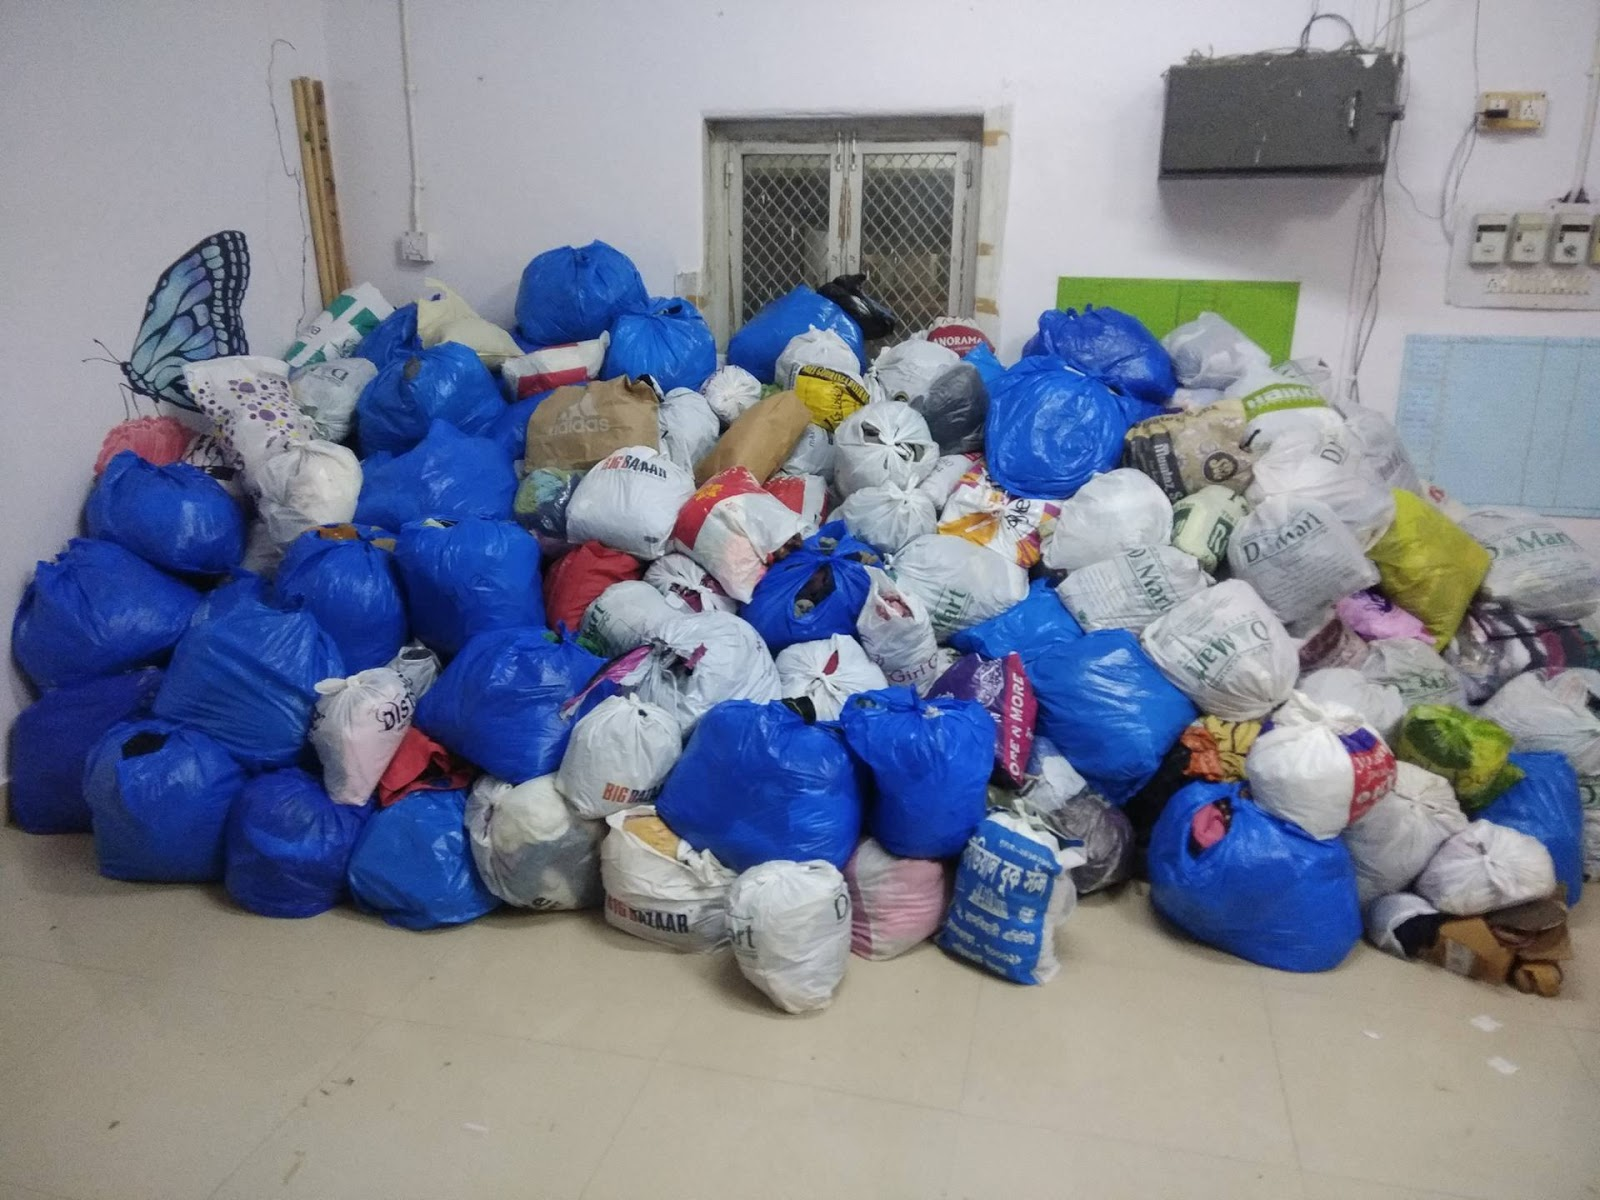
\includegraphics[width = 0.9\textwidth]{e10.jpg}
% \end{subfigure}%
% \begin{subfigure}{.5\textwidth}
% 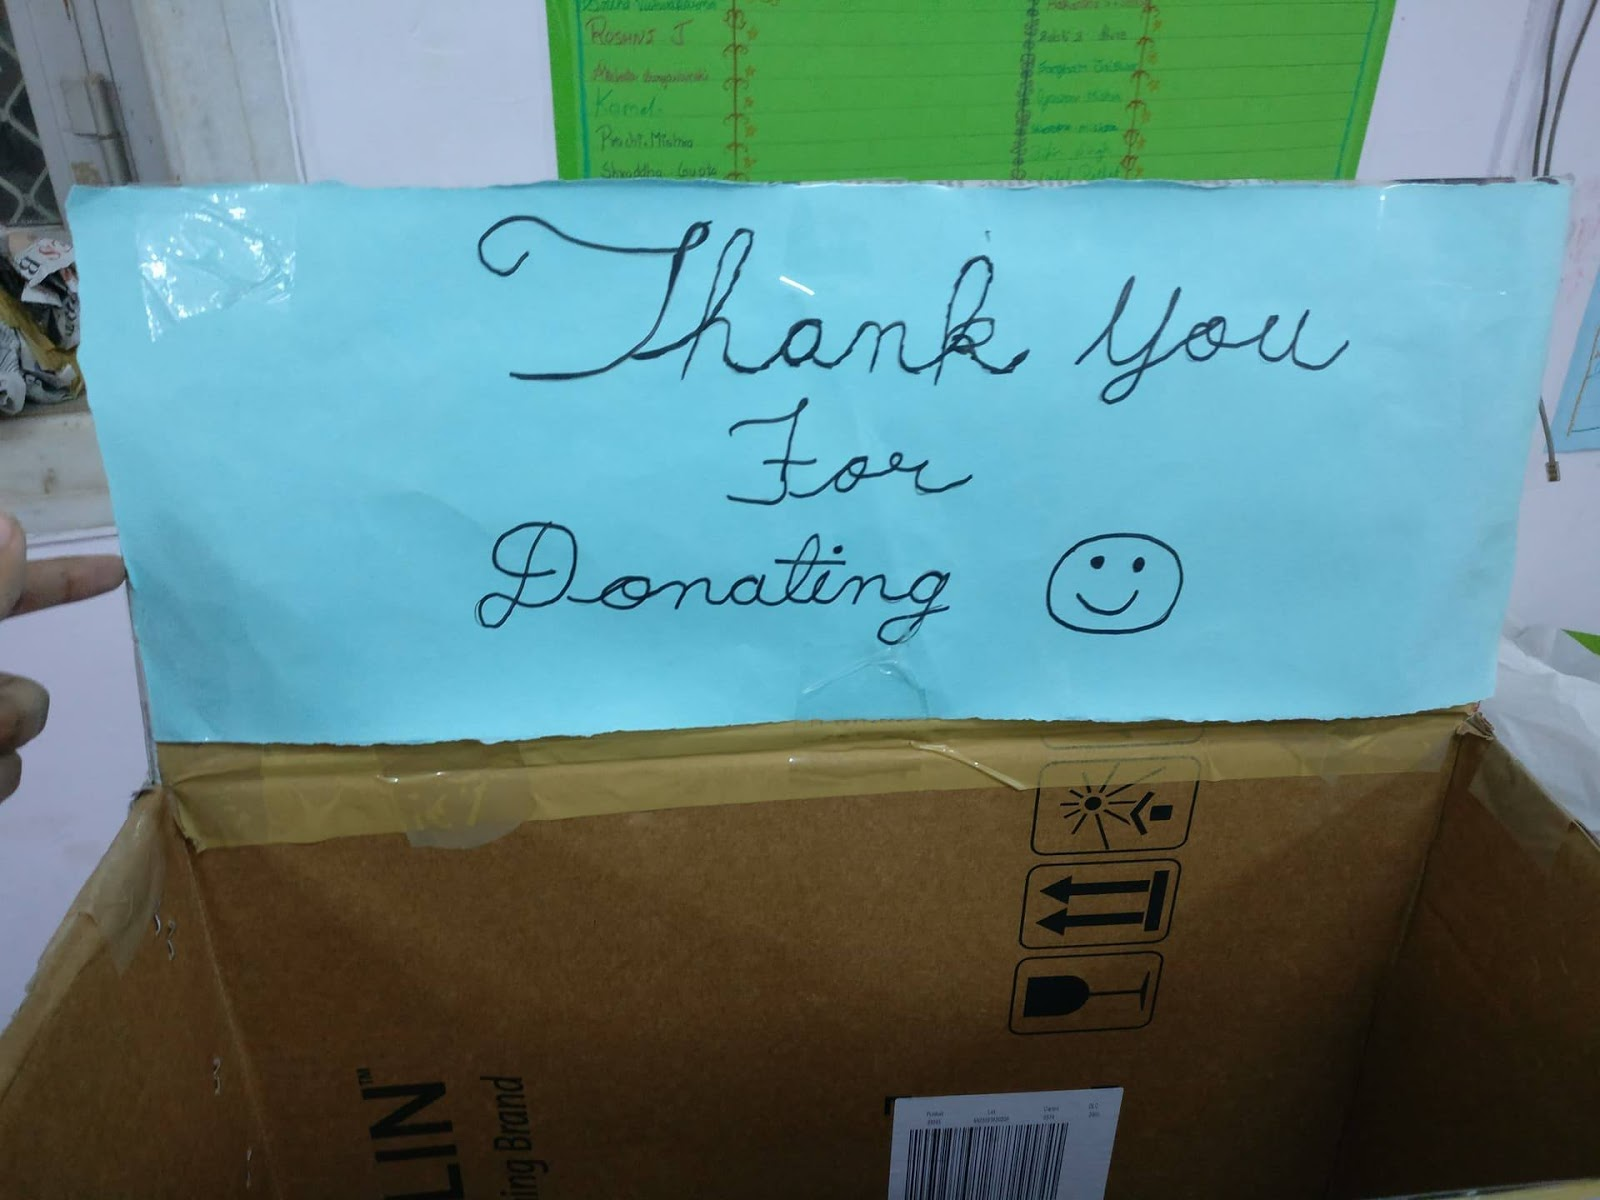
\includegraphics[width = 0.9\textwidth]{e6.jpg}
% \end{subfigure}
% \end{figure}

\addcontentsline{toc}{subsection}{NGO Visits}
\noindent \textbf {\Large \linebreak \linebreak \linebreak \linebreak \linebreak NGO Visits:}\\ \\“I can literally come and teach here daily, I truly love it!!”- An enthusiastic volunteer after a session \\ \\
Events department believes that apart from learning the basic subjects such as Maths and Science, a good bit of talking sense and correct use of language is also required to help students tackle the daily endeavors of life. Keeping this in mind, our volunteers visit different NGOs in and around the institute to inculcate in students, the basics of vocabulary and communication skills. The NGOs currently involved with us are The Logic Centre and Community Welfare Association(LCCWA) and Asha. The volunteers have a well prepared teaching module dedicated for the same and sessions are conducted over the weekend to teach different aspects of the above-mentioned topics, followed by an interactive activity to include the children and re-explaining the concept through direct participation. Thus, it is a fun activity for both the children and the volunteers. \\ \\
“Next time also, you come. I have many doubts, I will ask you to clear them and teach me other things.”-  A student at Asha
\\

\begin{figure}[H]
\centering
\begin{subfigure}{.5\textwidth}
 \centering
 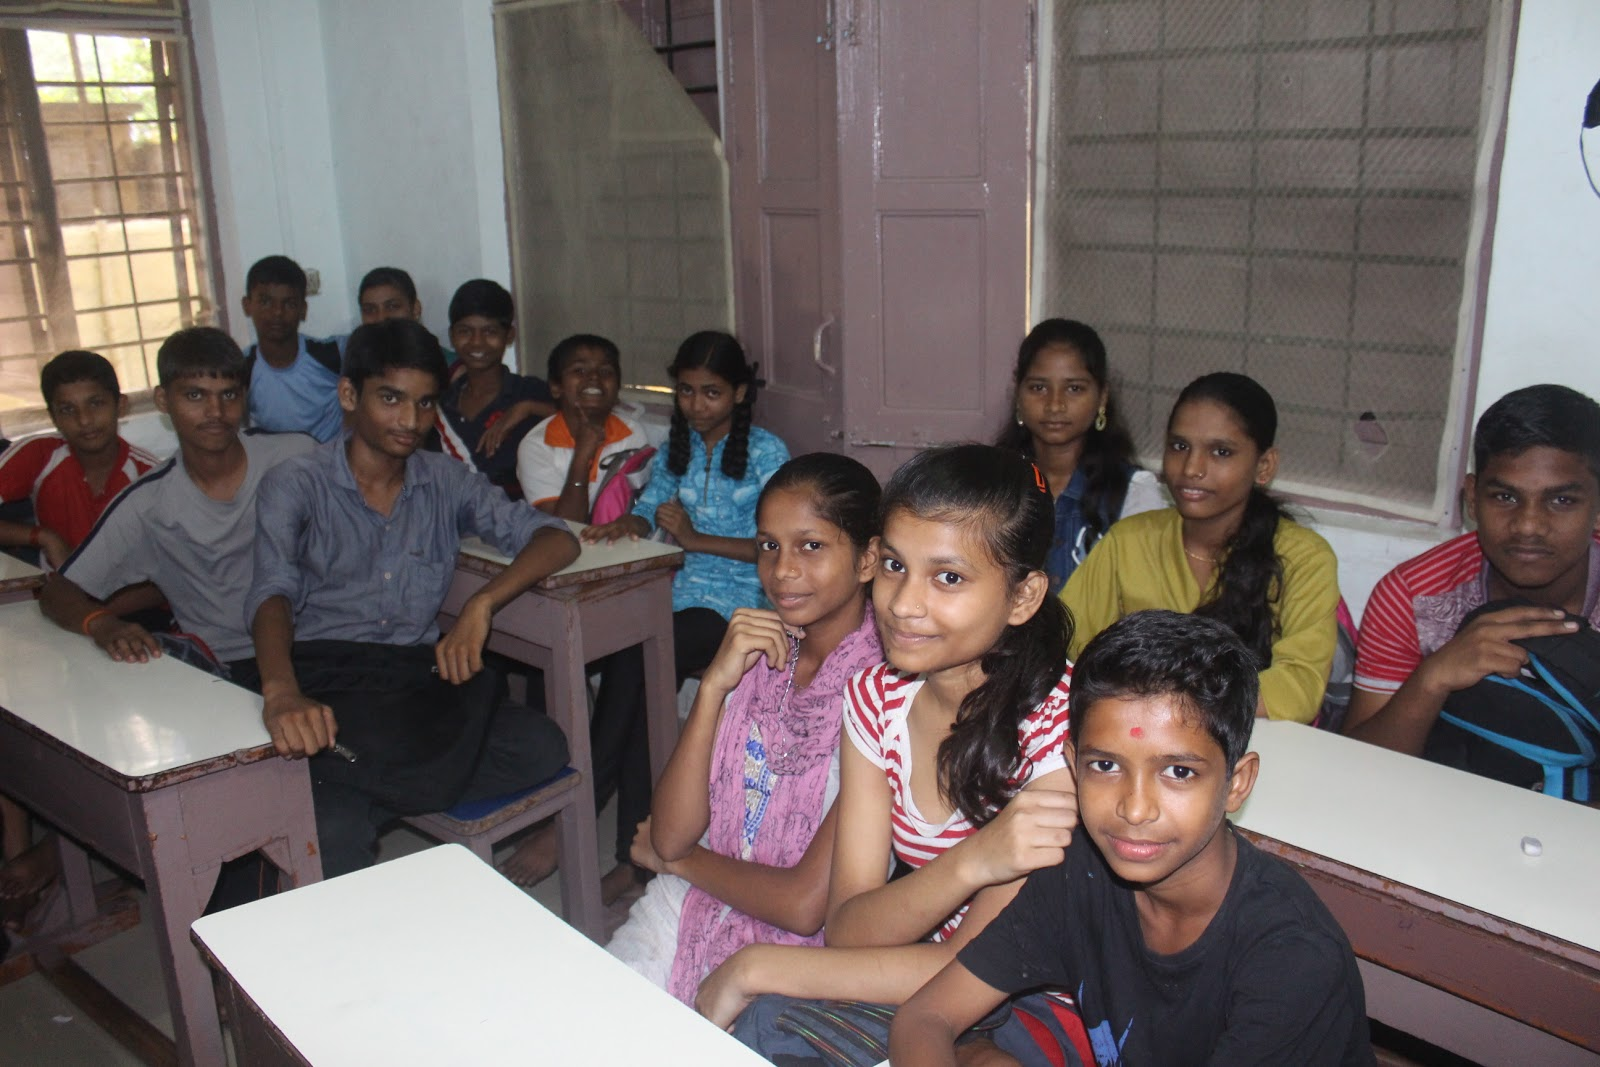
\includegraphics[width = 0.9\textwidth]{e9.jpg}
\end{subfigure}%
\begin{subfigure}{.5\textwidth}
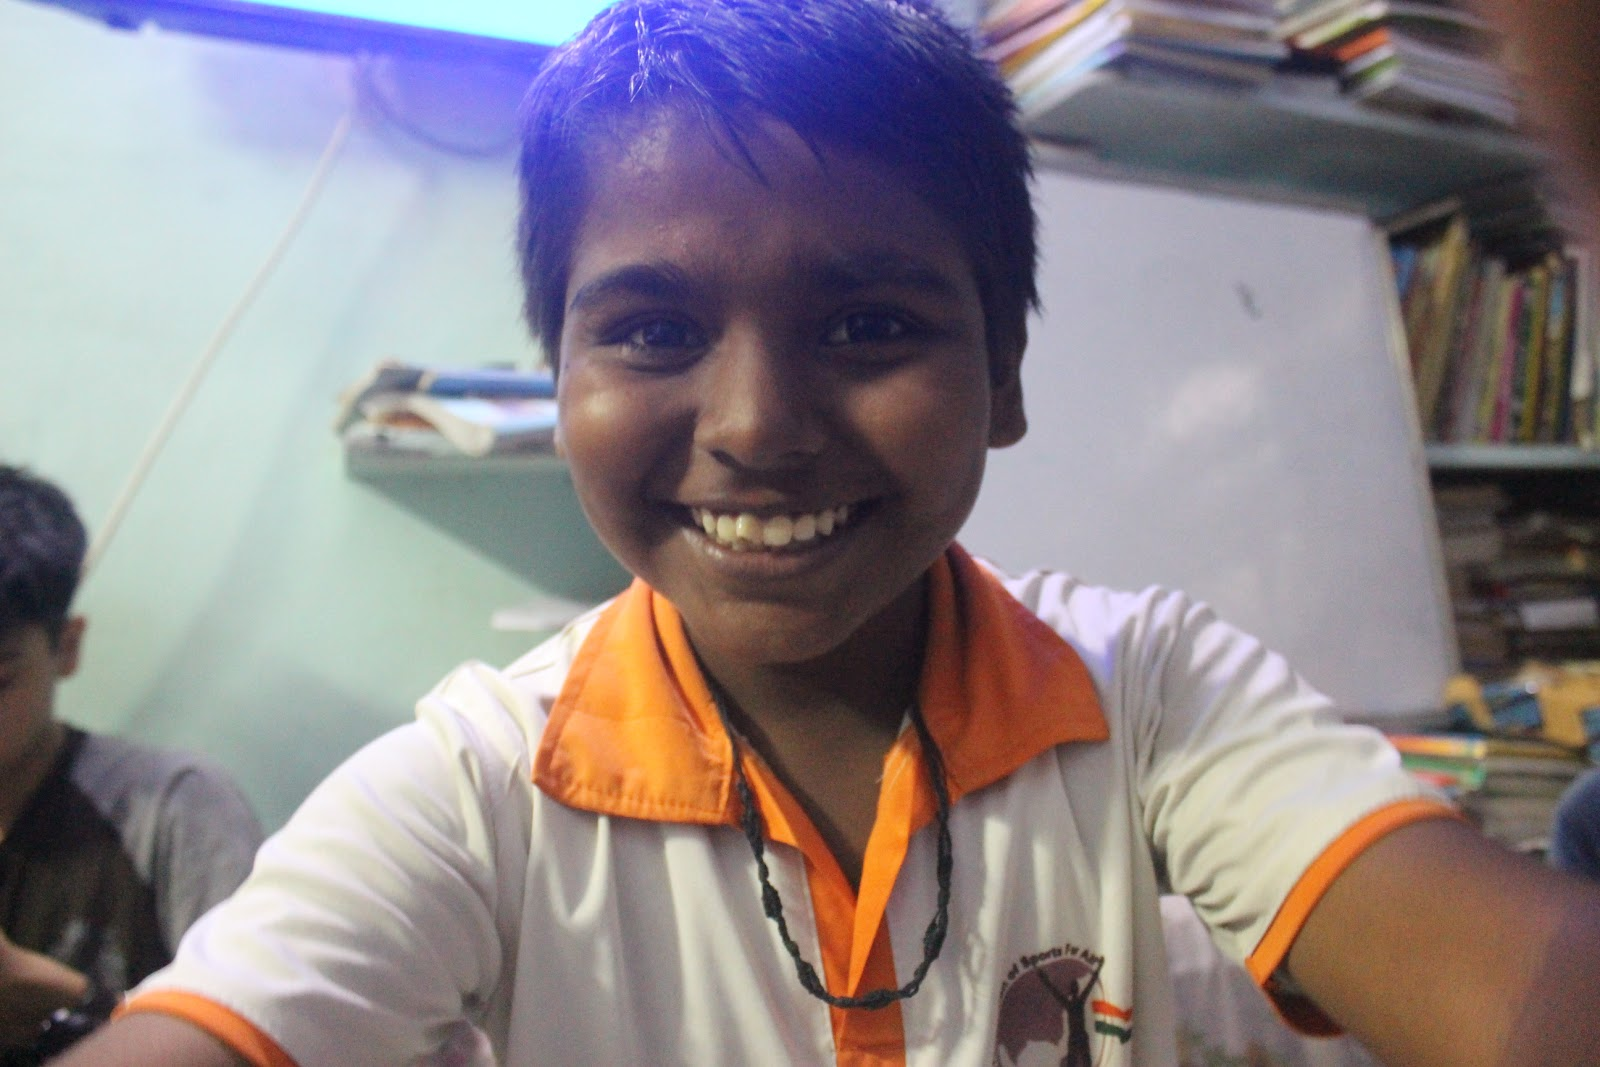
\includegraphics[width = 0.9\textwidth]{e11.jpg}
\end{subfigure}
\end{figure}

\begin{figure}[H]
\centering
\begin{subfigure}{.55\textwidth}
 \centering
 \includegraphics[width = 0.9\textwidth]{e12.jpg}
\end{subfigure}%
\begin{subfigure}{.5\textwidth}
\includegraphics[width = 0.9\textwidth]{e13.jpg}
\end{subfigure}
\end{figure}

\addcontentsline{toc}{subsection}{Meals Of Content}
\noindent \textbf {\Large \linebreak \linebreak \linebreak \linebreak \linebreak \linebreak  Meals Of Content:}\\ \\“Your initiative is truly innovative and new. I donate every day and love to do so.”- A post graduate student studying in the institute \\ \\
Meals of Content(MoC) is a new initiative launched by the Events department this year, to cash in on the fact that the canteens do not always provide the change and the buyer must sometime reluctantly take different items with them. The MoC provided an alternate platform for the same, purchasing biscuits from that change and donating it the donation boxes provided there by NSS. The first activity of the academic year for the volunteers, this included making of interactive donation boxes, coaxing the various canteen owners to allow the boxes to be kept in canteens, and then regular collection by the volunteers. This year, the initiative was held in some of the department canteens and some hostel canteens. As a trial run, the MoC was also held outside the institute, to cater to a more diverse audience. The total collection was close to 300 packets, donated at the Aman Day Care center in the institute and the Akshay Patra supported schools in Thane, as an additive to their morning breakfast. The initiative is planned to be extended and made more effective in the coming years.

\begin{figure}[H]
\centering
\includegraphics[width = 0.7 \textwidth]{e14.jpg}
\end{figure}

\addcontentsline{toc}{subsection}{(L)earn a Living}
\noindent \textbf {\Large \linebreak \linebreak \linebreak  (L)earn a Living:}\\ \\In the working market, there is always a shortage of skilled assistants in the shops. On the other hand, in the slum areas we have people who are qualified enough to work, but not so due to insufficient some extra, edge-providing skills or due to indulgence in bad activities. The initiative tries to act as link between the two. Uptill now, the initiative is not on ground yet, but the back-end job is almost complete. This includes making a completely different interactive teaching module for imparting the required skills, and a survey conducted in the shops of galleria to get an overview of the type of labor force and skill required by different categories of shopkeepers.


\chapter*{National Innovation Club}
\markboth{National Innovation Club}{National Innovation Club}
\addcontentsline{toc}{chapter}{National Innovation Club}

\addcontentsline{toc}{section}{About the Department}
\section*{ About the Department:}   We started with the name TechGSR (Tech Geek Social Responsibility) where we encouraged senior undergraduate and postgraduate students to find and implement
technical solutions to social problems.
TechGSR formed the precursor to establishing the National Innovation Club, the
student body of IIT Bombay which aims to build a sustainable system at IIT Bombay
which will promote the students of IIT Bombay to create technology for development of
society with a guidance from learned professors, established institutes and citizens of
India themselves and to create leaders and entrepreneurs in socio-tech field. We
encourage our undergraduate freshmen to work upon these projects. We are running
NIC as a department under NSS IIT Bombay

\vspace*{0.5cm}
\noindent \textbf{Link:} \url{https://gymkhana.iitb.ac.in/~nss} \\

\addcontentsline{toc}{section}{Smart Irrigation Control System}
\noindent\textbf{\Large \linebreak Smart Irrigation Control System:}\\ \\The existing irrigation system is tedious, time consuming and very wasteful in terms of
water usage, so we came up with this project which works towards effective irrigation
and prevention of water wastage in uncontrolled irrigation promoting water conservation
and reducing the environmental impacts.
\\ \\ This prototype avoids water wastage by providing only the required amount of water
needed based on the moisture level of the soil which is constantly monitored by
sensors. The data obtained from the sensors is processed by an Arduino
micro controller that signals a valve controlling the water flow.
We have also developed an user interface in form of an Android Application that
displays the current moisture levels of the soil and enables the user to change the
threshold values. The application connects with the Arduino micro controller using a
Bluetooth module.
\\ \\ We have implemented our working prototype in NSS nursery to observe the changes
with respect to other manually irrigated plants and to have an insight of moisture
requirements of plants.Currently, we are probing the possibilities of implementing our prototype in Hostel
Gardens of IITB and also working to scale up the use of our device over a larger area
with more sensors. \\ \\ \\

\begin{figure}[H]
\centering
\begin{subfigure}{.5\textwidth}
 \centering
 \includegraphics[width = 0.9\textwidth]{nic1.JPG}
\end{subfigure}%
\begin{subfigure}{.5\textwidth}
\includegraphics[width = 0.9\textwidth]{nic2.JPG}
\end{subfigure}
\caption*{Implementation of Smart Irrigation Control System in NSS Nursery}
\end{figure}

% \addcontentsline{toc}{section}{Walking Sticks for Blind:}
% \noindent\textbf{\Large Walking Sticks for Blind:}\\ \\The main objective of the project is to aid blind people to walk with ease and be warned
% of the presence of obstacles in their path. The main components of the device include
% an ultrasonic sensor that tracks the distance of obstacles in the vicinity of the user and
% an Arduino microcontroller that processes the information received from the ultrasonic
% sensors. We implemented a mechanism that causes the stick to vibrate whenever an
% obstacle is detected. This allows the user to be aware of the obstruction in the path and
% also enables them to navigate safely. We have also added new functionalities to the
% existing model such as rechargeable batteries and a charging port that allows the user
% to charge the walking stick.
% \noindent \textbf{Current Status:} We have completed the prototype of the Walking Stick for Blind and
% are now testing.\\ \\

\addcontentsline{toc}{section}{Projects for augmentation and value addition to grassroot innovations}
\noindent \textbf{\Large  Projects for augmentation and value addition to grassroot innovations:}\\ \\These includes taking existing working ideas and investigate how to even slightly
improve the existing working solution. It is therefore not about forcing our solutions
manufactured in labs but about complementing or supplementing existing solutions. All
of these problem statements were taken from NIF (National Innovation Foundation).\\ \\

% \noindent\textbf{\Large Hand Operated Water Lifting Pump :}\\ \\ N Shakthimaithan, an innovator from a town in Thiruvarur district, developed a hand
% operated water-lifting device device to irrigate fields from canal or pond and drain out
% excess water from cultivated land, with minimal effort.
% As residents of Mumbai, we observed that there were frequent short lived floodings due
% to heavy rains in the city. We took up the idea to transfer the technology used by N
% Shakthimaithan to the meet the urban needs.
% To understand the real need and requirements from such a product by an urban area,
% we conducted a number of surveys in nearby areas. We received positive feedbacks on
% the idea.
% On researching various mechanisms, we adopted the Reciprocating Mechanism
% which was best suited to our needs. We created a CAD model of the pump design and
% optimized its design to gain maximum work output. We also made the device more
% cheaper and portable.
% We are currently working on creating a prototype based on the improved designs.\\

% \addcontentsline{toc}{section}{Achievement so far }
% \noindent \textbf{\Large Achiements so far:}\\ \\{
% We were able to come up with the innovative ideas of the existing technical issues which were known through NIF. At the end of the semester all our efforts paid off. The department head of NIC (Akash Padmane) was invited to the Festival of innovation to present our projects. So Akash Padmane took represented NSS IIT Bombay at Festival of Innovation at the \textbf{Rashtrapati Bhavan}}


% \begin{figure}[H]
% \centering
% \includegraphics[width = 0.3\textwidth]{nic3.jpg}
% \caption*{NIC department head representing NSS IIT Bombay at Rashtrapati Bhavan}
% \end{figure}

\chapter*{\huge Media Coverage and Common Activities}
\markboth{Media Coverage and Common Activities}{Media Coverage and Common Activities}
\addcontentsline{toc}{chapter}{Media Coverage and Common Activities}

\pagebreak
\chapter*{\huge Media Coverage and Common Activities}


\pagebreak
\chapter*{\huge Media Coverage and Common Activities}


\pagebreak
\chapter*{\huge Media Coverage and Common Activities}


\pagebreak
\chapter*{\huge Media Coverage and Common Activities}


\pagebreak
\chapter*{\huge Media Coverage and Common Activities}


\chapter*{\huge Media Coverage and Common Activities}
\markboth{Media Coverage and Common Activities}{Media Coverage and Common Activities}
\addcontentsline{toc}{chapter}{Media Coverage and Common Activities}
\pagebreak

\chapter*{\huge Media Coverage and Common Activities}
\markboth{Media Coverage and Common Activities}{Media Coverage and Common Activities}
\addcontentsline{toc}{chapter}{Media Coverage and Common Activities}
\pagebreak

\chapter*{\huge Media Coverage and Common Activities}
\markboth{Media Coverage and Common Activities}{Media Coverage and Common Activities}
\addcontentsline{toc}{chapter}{Media Coverage and Common Activities}
\pagebreak


\chapter*{\huge Media Coverage and Common Activities}
\markboth{Media Coverage and Common Activities}{Media Coverage and Common Activities}
\addcontentsline{toc}{chapter}{Media Coverage and Common Activities}
\pagebreak


\chapter*{\huge Media Coverage and Common Activities}
\markboth{Media Coverage and Common Activities}{Media Coverage and Common Activities}
\addcontentsline{toc}{chapter}{Media Coverage and Common Activities}
\pagebreak

\chapter*{\huge Media Coverage and Common Activities}
\markboth{Media Coverage and Common Activities}{Media Coverage and Common Activities}
\addcontentsline{toc}{chapter}{Media Coverage and Common Activities}
\pagebreak


\chapter*{\huge Media Coverage and Common Activities}
\markboth{Media Coverage and Common Activities}{Media Coverage and Common Activities}
\addcontentsline{toc}{chapter}{Media Coverage and Common Activities}
\pagebreak


\chapter*{\huge Media Coverage and Common Activities}
\markboth{Media Coverage and Common Activities}{Media Coverage and Common Activities}
\addcontentsline{toc}{chapter}{Media Coverage and Common Activities}
\pagebreak


\chapter*{\huge Media Coverage and Common Activities}
\markboth{Media Coverage and Common Activities}{Media Coverage and Common Activities}
\addcontentsline{toc}{chapter}{Media Coverage and Common Activities}
\pagebreak

\chapter*{\huge Media Coverage and Common Activities}
\markboth{Media Coverage and Common Activities}{Media Coverage and Common Activities}
\addcontentsline{toc}{chapter}{Media Coverage and Common Activities}
\pagebreak

\chapter*{\huge Media Coverage and Common Activities}
\markboth{Media Coverage and Common Activities}{Media Coverage and Common Activities}
\addcontentsline{toc}{chapter}{Media Coverage and Common Activities}
\pagebreak

\chapter*{\huge Media Coverage and Common Activities}
\markboth{Media Coverage and Common Activities}{Media Coverage and Common Activities}
\addcontentsline{toc}{chapter}{Media Coverage and Common Activities}
\pagebreak


\chapter*{\huge Media Coverage and Common Activities}
\markboth{Media Coverage and Common Activities}{Media Coverage and Common Activities}
\addcontentsline{toc}{chapter}{Media Coverage and Common Activities}

\addcontentsline{toc}{section}{Media Coverage}
\section*{ Media Coverage:}   NSS, IIT Bombay has always been setting an example in diverse spheres of social welfare activities and is playing a major role in making common people aware about the importance of harmony in the society, the nation and the world. The International as well as Indian Media plays a huge role in this direction by covering our activities and events for all the common people to know. We genuinely feel reaching out with our activities to the common people through media helps create an awareness among people regarding the importance of self-contribution for the welfare and upliftment of the society. Some of our activities were published in national and international news reports.

\begin{figure}[H]
\centering
\includegraphics[width = 1 \textwidth]{d1.jpg}
\caption*{The Cloth Collection Campaign covered by the Hindustan Times}
\end{figure}

\begin{figure}[H]
\centering
\includegraphics[width = 0.8 \textwidth]{d3.png}
\caption*{New activities covered in the Campus Diary, IIT Bombay}
\end{figure}

\begin{figure}[H]
\centering
\includegraphics[width = 0.6 \textwidth]{d4.jpg}
\caption*{Open Learning Initiative (OLI) published on India Today}
\end{figure}

The modern day Social Media is definitely a huge pool of people to reach out and create an impact through our activities. NSS, IIT Bombay has been quite active on several social media platforms like Facebook, YouTube, Wordpress Blog and many more. The primary motive of using social media for increasing outreach of NSS, IIT Bombay is reaching out
to the exponentially growing user base after digitalisation. \\ \\  We believe, through awareness among people, at some corner of their thoughts, we instill in them a
feeling of doing something for the welfare of the society at a basic level. Social media provides a huge platform to reach out to nooks and corners nationally as well as internationally because of a huge user base.

\begin{figure}[H]
\centering
\includegraphics[width = 0.8 \textwidth]{d2.png}
\caption*{Reaching out to 12k+ people}
\end{figure}

\addcontentsline{toc}{section}{Common Activities}
\section*{ \LARGE Common Activities:}
\section*{ The Artistic Impact:} A pen, a brush and a camera. All three of these are powerful tools to shed light on social problems and create awareness among the masses. The Artistic Impact is a nationwide Socio-Art competition conducted by NSS, IIT Bombay with a motivation of capturing the creativity of the young minds of India to highlight social issues. This competition has three segments: ‘ThINK’, ‘Social Canvas’, and ‘Click for Change’. With a bright start to this initiative last year, we received tremendous participation this year too with participants from states so far as Haryana and Orissa. The winners (3, 3, 10 from Social Canvas, Click for Change and ThINK genres, respectively) were awarded with certificate and official merchandise of NSS, IIT Bombay.

\begin{figure}[H]
\centering
\includegraphics[width = 0.8 \textwidth]{a1.jpg}
\caption*{Award winning entry in ‘Social Canvas’, the judicial system trying to protect women from devils
}
\end{figure}

\section*{ All NSS Meet:} On April 7th, NSS IIT Bombay organized ‘All NSS Meet’ for Mumbai units. 13 representatives of other NSS units from different regions of Mumbai attended this event. All participants were overwhelmingly enthusiastic about participating in this event. During the event, we introduced all our activities along with a discussion of what all activities can be carried out collectively to reach out more beneficiaries. It was followed by a dance performance by Muskaan kids from the NGO LCCWA. It was then followed by the presentations of the other NSS units’ for mutual learning. Informal discussions were done during the snacks break from which we came to know the scope of reaching out to them through our activities. Finally, we concluded the event mentioning a few activities that could be taken forward by all the colleges. NSS IIT Bombay is grateful to all these NSS units’ for dedicating their precious time and making this event a success. We are looking forward to involve more number of colleges so that services could be extended to maximum regions of Mumbai.

\begin{figure}[H]
\centering
\includegraphics[width = 0.8 \textwidth]{a2.jpg}
\caption*{All NSS Meet with the representatives from 6 NSS units in Mumbai}
\end{figure}

\section*{ Jammu and Kashmir kids’ visit to IIT Bombay:} A day was spent with the 11th class students of Jammu and Kashmir.
These kids from Jammu and Kashmir Govt schools came to the institute to know the
lifestyle of IITB students and also to know more about the culture
here in Mumbai. This was the first time they were coming out of their
state. \\
  In this four days of tour, apart from academics and lab visits, they
got to know about the various extra curricular activities that
the students here do.\\ \\
    NSS IIT Bombay volunteers thought of engaging them in an institute tour
and made them feel happy by letting them interact with NGO kids
through Muskaan and Prayog session. So in the first half, kids were taken along
for an institute tour starting from Nursery-lakeside-boathouse, after a
short orientation. In the second half, we had Fine arts session in the
Muskaan and Science experiments in Prayog along with the NGO kids.
\begin{figure}[H]
\centering
\includegraphics[width = 0.65 \textwidth]{a3.jpg}
\caption*{NSS Volunteers with kids from Jammu and Kashmir while Institute tour
}
\end{figure}

\section*{ Invisible Humans of IIT Bombay:} This is a series of posts featuring unheard stories of the people of campus whom majority of the residents know by face but nobody cares about their story. These people make our lives better at the campus and we think it is our duty to bring their stories and their dreams into the light. Our activity associates identified many such people including a Bhutta Stall owner, Dhobi of Hostels, Librarian, SAC store incharge, Assistant Sports officer, friendly mess workers of hostel 10 etc. The student community of IIT Bombay likes these stories of people they see daily and we got positive feedback from them.

\begin{figure}[H]
\centering
\includegraphics[width = 0.65 \textwidth]{a4.jpg}
\caption*{Mr. Shankar Gupta (KReSIT Samosa wale) being covered in the series ‘Invisible Humans of IIT Bombay’
}
\end{figure}

\section*{World Menstrual Hygiene Day Awareness: }Menstrual Hygiene is considered as a huge taboo in the Indian society. Considering this, NSS IITB decided to break the taboo about menstrual hygiene by initiating an awareness drive through social media platforms. The awareness drive reached to more than 52,000 people throughout the nation.

\begin{figure}[H]
\centering
\includegraphics[width = 0.75 \textwidth]{a6.png}
\end{figure}

\section*{Memoirs: } Memoirs are the excerpts from well-written essays by NSS volunteers. Most of these are a way for the volunteers to sit back and cherish the memories they volunteer(s) had.

\begin{figure}[H]
\centering
\includegraphics[width = 0.75 \textwidth]{a5.jpg}
\caption*{Memoirs: Volunteer experience summarised!}
\end{figure}



\chapter*{Team NSS 2017-18}
\markboth{Team NSS 2017-18}{Team NSS 2017-18}
\addcontentsline{toc}{chapter}{Team NSS 2017-18}

\vspace*{0.8cm}

\noindent \textbf{\Large Faculty Coordinators:}\\
Prof. Anand B. Rao\\
Prof. Ganesh Ramakrishnan\\ \\
\noindent \textbf{\Large Overall Coordinator:}\\
Barre Prathyusha \\\\
\noindent \textbf{\Large Department Heads:}\\ \\
\textbf{\large Educational Outreach:}\\
Balreen Saini \\
Saugata Haldar\\ \\
\textbf{\large Green Campus:}\\
Mainak Saha\\
Pragya Valay\\ \\
\textbf{\large Vikas:}\\
Mohak Sahu\\
Kesha Tamakuwala\\ \\
\textbf{\large Events:}\\
Aadarsh Parashar \\
Vaidehi Mahajan\\ \\
\textbf{\large National Innovation Club:}\\
Akash Padmane\\ \\
\textbf{\large Design and Media:}\\
Suyash Bagad\\
Fatima Salehbhai\\ \\
\textbf{\large Web and Finance:}\\
Sunil B\\ \\



\noindent \textbf{\Large Activity Associates:}\\ \\
\noindent \textbf{\large Educational Outreach:}\\
Aditya Saurabh\\
Akshata Dalvi\\
Aniket Prajapati\\
Hemant Kumawat\\
Himani Gangurde\\
Kavya Bhandari\\
Manan Agarwal\\
Nitin Kumar Tiwari
\\
Yash Kadam
\\ \\

\pagebreak

\noindent \textbf{\Large Green Campus:}\\
Aniket Pawan Dubey\\
Hiranyagarbh A Narale\\
Debanjali Chatterjee\\
Mayank Sultania\\
Mohish Shah\\
Mohana Madhumita Pokkuluri
\\
Tanay Wagh\\ \\
\noindent \textbf{\large Vikas:}\\
Anshul Verma \\
Ishita Das \\
Jovina Vaswani \\
Sowmya Ravichandran
 \\
Ritesh Goenka \\
Vinayak Gupta\\ \\

\noindent \textbf{\large Events:}\\
Nautatva Navlakha \\
Pratyush Ragini Singh\\
Puneet Nemade\\
Yash T. Rajan\\
\\
\noindent \textbf{\large National Innovation Club:}\\
Sagar Seth \\
Amit Kumar \\ \\
\noindent \textbf{\large Design and Media:}\\
Aditya Dev\\
Bhargavi\\
Kushal Mittal\\
Sahiram Tada\\ \\
\noindent \textbf{\large Web:}\\
Y.V.Sriram\\


\end{document}
